
\chapter{}

\heading{ಮೊದಲಿಗೆ}

ಚಂದ್ರಶೇಖರ ವೆಂಕಟ ರಾಮನ್ (\enginline{C. V. Raman}), ಜಗತ್ತೇ ಬೆರಗುಗೊಳ್ಳುವಂತೆ, ಈಗ ತಮ್ಮ ಹೆಸರಿನಲ್ಲಿರುವ “ಬೆಳಕಿನ ಚದರುವಿಕೆಯಲ್ಲಿನ ರಾಮನ್ ರೇಖೆಗಳ” ಆವಿಷ್ಕಾರದ ಪ್ರಕಟಣೆಯನ್ನು \enginline{1928}ರಲ್ಲಿ ಮಾಡಿದರು. ಏಳು ವರ್ಷಗಳ ಸತತ ಸಂಶೋಧನೆಯ ಫಲವಾಗಿ ರಾಮನ್ ಮತ್ತು ಅವರ ತಂಡದ ವಿದ್ಯಾರ್ಥಿಗಳು ಮತ್ತು ಸಹವರ್ತಿಗಳಿಗೆ ಈ ಸಿದ್ಧಿ ಲಭಿಸಿತ್ತು.

\vskip 2pt

ಈ ಆವಿಷ್ಕಾರ ಪ್ರಕಟಗೊಂಡ ಕೆಲವೇ ದಿನಗಳಲ್ಲಿ ಮೇರಿಲ್ಯಾಂಡ್ ರಾಜ್ಯದ ಬಾಲ್ಟಿಮೋರ್ ನಲ್ಲಿರುವ ಜಾನ್ ಹಾಪ್‍ಕಿನ್ಸ್ ಯೂನಿವರ್ಸಿಟಿಯಲ್ಲಿನ ಪ್ರೊಫೆಸರ್ \enginline{R. W.} ವುಡ್ ರವರು \textit{ನೇಚರ್} ಪತ್ರಿಕೆಗೆ ಒಂದು ಸಂದೇಶವನ್ನು ಕಳುಹಿಸಿದರು. ಅದರಲ್ಲಿ ಈ ಒಕ್ಕಣೆಯಿತ್ತು.

\vskip 2pt

‘ಪಾರದರ್ಶಕ ವಸ್ತುಗಳ ಮೂಲಕ ಅತಿಶಕ್ತಿಯುತ ಏಕ ತರಂಗಾವರ್ತದ ಬೆಳಕನ್ನು ಹಾಯಿಸಿದಾಗ ಅಣುಗಳು ಬೆಳಕನ್ನು ಮಾರ್ಪಡಿಸಿ, ಭಿನ್ನ ತರಂಗಾವರ್ತದಲ್ಲಿ ಚದರಿಸುತ್ತವೆಯೆಂಬ ಆಶ್ಚರ್ಯಕರ ಮತ್ತು ಪ್ರಖರ ಧೀ ಶಕ್ತಿಯಿಂದಾದ ಈ ಆವಿಷ್ಕಾರವು ಹಲವಾರು ಬಗೆಯ ಅಣು ಸಂರಚನಾ ಅಧ್ಯಯನಗಳಿಗೆ ಸಹಾಯ ಮಾಡುತ್ತದೆ. ಅಣುಗಳು ಸೂಸಿದ ಬೆಳಕಿನ ತರಂಗಾವೃತ್ತಿಗೂ, ಅದಕ್ಕೆ ಹಾಯಿಸಿದ ಬೆಳಕಿನ ತರಂಗಾವೃತ್ತಿಗೂ ಇರುವ ವ್ಯತ್ಯಾಸವು, ಅವಕೆಂಪು ಶೋಷಣ ರೋಹಿತಪಟ್ಟಿಯ (\enginline{absorption band}), ತರಂಗಗಳ ಆವೃತ್ತಿಗೆ ಸರಿಹೊಂದುತ್ತದೆ ಎಂಬ ಅಂಶವು ಅದ್ಭುತ ಆವಿಷ್ಕಾರ. ನಾನು ಈ ಆವಿಷ್ಕಾರವನ್ನು ಪರೀಕ್ಷಿಸಿ ಋಜುವೆಂದು ಸಾಬೀತುಪಡಿಸಿದ್ದೇನೆ....... ಇದು ಅತಿ ಸುಂದರ ಆವಿಷ್ಕಾರ. ಬೆಳಕಿನ ಚದರಿಕೆಯ ಬಗ್ಗೆ ರಾಮನ್‍ರವರು ಬಹಳ ತಾಳ್ಮೆಯಿಂದ ಅನೇಕ ವರ್ಷಗಳಿಂದ ಸಂಶೋಧನೆಯಲ್ಲಿ ತೊಡಗಿಸಿಕೊಂಡಿದ್ದಾರೆ. ಆಧುನಿಕ ಕ್ವಾಂಟಂ ಸಿದ್ಧಾಂತಕ್ಕೆ, “ರಾಮನ್ ಪರಿಣಾಮ”ವು ಸಾಕ್ಷ್ಯವನ್ನು ಒದುಗಿಸುತ್ತದೆ’.

\vskip 2pt

ಇಲ್ಲಿ ಗಮನಿಸಿಬೇಕಾದ ಅಂಶವೆಂದರೆ, ಇಂತಹ ಮಹತ್ತರ ಸಂಶೋಧನೆಯನ್ನು ರಾಮನ್‍\break ರವರು \enginline{500} ರೂ ಗಳಿಗೂ ಹೆಚ್ಚಿಲ್ಲದ ಮೌಲ್ಯದ ಉಪಕರಣಗಳ ಮೂಲಕ ಸಾಧಿಸಿದರು. ಜಗತ್ತಿನ\break ಬೆರಳಣಿಕೆಯ ಮಂದಿ ವಿಜ್ಞಾನಿಗಳು ಇಂತಹ ಗಂಭೀರ ಆವಿಷ್ಕಾರಗಳನ್ನು ಅತಿ ಕಡಿಮೆ ಮೌಲ್ಯದ ಪರಿಕರಗಳನ್ನು ಉಪಯೋಗಿಸಿ ಮಾಡುವುದರಲ್ಲಿ ಸಫಲರಾಗಿದ್ದಾರೆ.

ಏಪ್ರಿಲ್ \enginline{1931}ರಲ್ಲಿ ಪ್ರಕಟವಾದ ಬೆಲ್ ಲ್ಯಾಬೊರೇಟರೀಸ್ ರೆಕಾರ್ಡ್ ನಿಯತಕಾಲಿಕದಲ್ಲಿ, ಮುಂದೆ \enginline{1937}ರಲ್ಲಿ ನೊಬೆಲ್ ಪಾರಿತೋಷಕವನ್ನು \enginline{G. P.} ಥಾಮ್‍ಸನ್ ರವರೊಡನೆ ಜಂಟಿಯಾಗಿ ಪಡೆದ \enginline{C. J.} ಡೇವಿಡ್‍ಸನ್ ರವರು “ಸರ್. ಚಂದ್ರಶೇಖರ ವೆಂಕಟ ರಾಮನ್ ನೊಬೆಲ್ ವಿಜೇತರು” ಎಂಬ ಶೀರ್ಷಿಕೆಯಡಿಯಲ್ಲಿ ಹೀಗೆ ಬರೆದರು:\enginline{-}

“ರಾಮನ್‍ರವರು ಮಾಡಿದ ಸರಳ ಪ್ರಯೋಗವನ್ನು ಯಾವ ಪ್ರಯೋಗಾಲಯದಲ್ಲಾದರೂ ಯಾರು ಬೇಕಾದರೂ ಮಾಡಬಹುದಿತ್ತು ಎನ್ನುವ ಮಾತು ಈ ಮುಂಚಿನಿಂದಲೂ ಕೇಳಿಬರುತ್ತಿದೆ. ಈ ಪ್ರಯೋಗವನ್ನು ರಾಮನ್ ಅವರೇ ಏಕೆ ಮಾಡಿದರು ಎಂಬುದು ಆಕಸ್ಮಿಕವೇನಲ್ಲ. ಭೌತಶಾಸ್ತ್ರದಲ್ಲಿ ಬಹುಮುಖ್ಯ ಆವಿಷ್ಕಾರಗಳು, ಅದರಲ್ಲೂ ಸರಳ ಸಂಶೋಧನೆಗಳನ್ನು ಯಾರು ಭಾವತೀವ್ರತೆಯಿಂದ ವಿಜ್ಞಾನ ವಿಷಯದಲ್ಲಿ ಮಗ್ನರಾಗಿರುತ್ತಾರೋ ಅವರೇ ಮಾಡಲು ಸಾಧ್ಯವಾಗುತ್ತದೆ. ಇದು ಈ ಪ್ರಸಂಗದಲ್ಲೂ ನಿಜ”.

ಇದೇ ಲೇಖನದಲ್ಲಿ ಅವರು ಬರೆಯುತ್ತಾರೆ:\enginline{-}

“ಭಾರತದಲ್ಲಿ ವಿಜ್ಞಾನದ ಬೆಳವಣಿಗೆಗೆ, ರಾಮನ್‍ರವರ ಸಾಧನೆಯು ಒಳ್ಳೆಯ ಮಾದರಿ ಸೃಷ್ಟಿಸುತ್ತದೆ. ಏಕೆಂದರೆ ರಾಮನ್‍ರವರು ತಮ್ಮ ಔನ್ನತ್ಯವನ್ನು ಭಾರತದಲ್ಲಿದ್ದುಕೊಂಡೇ ಸಾಧಿಸಿದರು. ಅವರಿಗೆ ಹೊರದೇಶಗಳ ವಿಜ್ಞಾನಿಗಳ ಸಂಪರ್ಕವೂ, ಅಧ್ಯಯನವೂ ಅತ್ಯಲ್ಪ. ಅವರ ಶಿಕ್ಷಣವೆಲ್ಲವೂ ಅವರ ದೇಶದಲ್ಲಿಯೇ ಆಯಿತು. ಒಂದು ವರ್ಷಕಾಲ ಹೊರತುಪಡಿಸಿದರೆ ಅವರ ಜೀವನವೆಲ್ಲವೂ ಭಾರತದಲ್ಲೇ ಸಾಗಿದೆ. \enginline{1924}ರಲ್ಲಿ ಟೊರೆಂಟೋದಲ್ಲಿ ಬ್ರಿಟಿಷ್ ಅಸೋಸಿಯೇಷನ್ ವಿಜ್ಞಾನಿಗಳ ಕೂಟ ನಡೆದಾಗ ಅವರು ಬಂದಿದ್ದರು. ಇದಾದನಂತರ ಕೆಲವು ತಿಂಗಳ ಕಾಲ ಕ್ಯಾಲಿಫೋರ್ನಿಯಾ ಇನ್ಸ್ಟಿಟ್ಯೂಟ್ ಆಫ್ ಟೆಕ್ನಾಲಜಿಯಲ್ಲಿ ಸಂಶೋಧನೆ ಮಾಡಿದರು”.

ರಾಮನ್‍ರವರು ಅಪ್ಪಟ ಸ್ವದೇಶಿ ಪ್ರತಿಭಾಶಾಲಿ. ಭಾರತವನ್ನು ಜಗತ್ತಿನ ವೈಜ್ಞಾನಿಕ ಭೂಪಟದಲ್ಲಿ ದಾಖಲಿಸಿದರು. ಭಾರತದ ವೈಜ್ಞಾನಿಕ ರಂಗದಲ್ಲಿ ಆರು ದಶಕಗಳಿಗೂ ಹೆಚ್ಚು ಕಾಲ ತಮ್ಮ ಛಾಪು ಮೂಡಿಸಿದರು. ಭಾರತದ ಮಟ್ಟಿಗೆ ರಾಮನ್‍ರವರ ಜೀವನಗಾಥೆಗೆ ಸರಿಸಮರು ಇಲ್ಲ. ಅವರ ಬೃಹತ್ ಸಾಧನೆಗೆ, ಅವರ ವ್ಯಕ್ತಿತ್ವದಲ್ಲಿನ ಗುಣಗಳಾದ, ಮಿತಿಯರಿಯದ ಅಂತಃಶಕ್ತಿ ಮತ್ತು ಗುರಿ ತಲುಪಲು ಅವರಿಗಿದ್ದ ಅಪರಿಮಿತ ಉತ್ಸಾಹಗಳೇ ಕಾರಣವೆಂದು ಬೆರಳು ಮಾಡಿ ತೋರಿಸಬಹುದು. ಮ್ಯಾಕ್ಸ್ ಬಾರ್ನ್ ರವರು, ರಾಮನ್‍ರವರ ಬಗೆಗೆ ಹೀಗೆಂದಿದ್ದರು. \enginline{—} “ರಾಮನ್‍ರವರನ್ನು ಸರಿಗಟ್ಟುವ ವಿಜ್ಞಾನಿಗಳು ಭಾರತದಲ್ಲಿಲ್ಲ. ಅವರ ಭಾವತೀವ್ರತೆ ಮತ್ತು ಅಂತಃಶಕ್ತಿಗಳಿಗೆ ಯಾರೂ ಸಮರಿಲ್ಲ. ಯುರೋಪಿನಲ್ಲಿ ಕಾಣಬಹುದಾದ ಈ ಗುಣಗಳು ಭಾರತೀಯ ಸಾಮಾನ್ಯ ವಿಜ್ಞಾನಿಗೆ ಅವರ ಬಗ್ಗೆ ಗುಮಾನಿ ಮೂಡಿಸಬಹುದು”.

ಆದಿಯಿಂದಲೂ ರಾಮನ್‍ರವರು ಸ್ವತಂತ್ರ ಆಲೋಚನೆಗೆ ಅಸಾಮಾನ್ಯ ಸಾಮರ್ಥ್ಯ ತೋರಿಸತೊಡಗಿದರು. ಅವರು ವೈಜ್ಞಾನಿಕ ಸಂಶೋಧನೆಗೆ ಕೈಇಟ್ಟಾಗ ಅದರ ಸಫಲತೆಯ ಬಗ್ಗೆ ಅದಮ್ಯ ಭರವಸೆ ಹೊಂದಿರುತ್ತಿದ್ದರು. ಸೂಯೆಜ್ ಕಾಲುವೆಯಿಂದ ಈಚೆಗೆ ನೊಬೆಲ್ ಪುರಸ್ಕಾರ ಬರುವಂತೆ ಮಾಡುತ್ತೇನೆಂದು ಹೇಳುತ್ತಿದ್ದರು. ರಬೀಂದ್ರನಾಥ ಟಾಗೂರರು \enginline{1913}ರಲ್ಲಿ ಸಾಹಿತ್ಯಕ್ಕಾಗಿ ನೊಬೆಲ್ ಪಡೆದ ಏಷ್ಯಾದ ಪ್ರಥಮ ಪ್ರಜೆ ಎನಿಸಿದರು. ರಾಮನ್‍ರವರು ವಿಜ್ಞಾನ ಕ್ಷೇತ್ರದಲ್ಲಿ ನೊಬೆಲ್ ಪಡೆದ ಏಷ್ಯಾದ ಪ್ರಥಮ ಪ್ರಜೆಯಾಗಿದ್ದಾರೆ. ಅವರಿದ್ದ ಕಾಲ ಮತ್ತು ಸಂದರ್ಭಗಳನ್ನು ನೆನಸಿಕೊಂಡರೆ, ರಾಮನ್‍ ಅವರ ಹೊರತು ಈ ಹೇಳಿಕೆ ನೀಡಲು ಯಾರಿಗೂ ಸಾಧ್ಯವಿರಲಿಲ್ಲ.

ರಾಮನ್‍ರವರು \enginline{1888}ರ ನವೆಂಬರ್ \enginline{7}ರಂದು ದಕ್ಷಿಣ ಭಾರತದಲ್ಲಿ ಜನಿಸಿ \enginline{1970}ರ ನವೆಂಬರ್ \enginline{21}ರಂದು ಕಾಲವಾದರು. ತಮ್ಮ ಕೊನೆಗಾಲದವರೆಗೂ ವಿಜ್ಞಾನ ಕಾರ್ಯದಲ್ಲಿ ತೊಡಗಿಸಿಕೊಂಡಿದ್ದರು. \enginline{1988}ರಲ್ಲಿ ರಾಮನ್‍ರವರ ಶತಮಾನೋತ್ಸವ ಮತ್ತು ಅವರ ‘ರಾಮನ್ ಎಫೆಕ್ಟ್’ ಆವಿಷ್ಕಾರದ ವಜ್ರಮಹೋತ್ಸವವೂ ಒಟ್ಟಿಗೆ ಬಂದವು.


\heading{ಬ್ರಿಟಿಷ್ ಆಡಳಿತ ಮತ್ತು ಭಾರತದಲ್ಲಿ ವಿಜ್ಞಾನದ ಪರಿಸರ}

ಭಾರತದ ಸಂಸ್ಕೃತಿಯು ಅತಿ ಪುರಾತನವಾದದ್ದು. ಸಾವಿರಾರು ವರ್ಷಗಳ ಇದರ ಅಸ್ತಿತ್ವದಲ್ಲಿ ಅನೇಕ ಋಷಿಗಳು, ಪಂಡಿತರು, ಪ್ರತಿಭಾಶಾಲಿಗಳು, ಧಾರ್ಮಿಕಗುರುಗಳು ಆಗಿ ಹೋಗಿದ್ದಾರೆ. ವಿಜ್ಞಾನ ಮತ್ತು ಗಣಿತಗಳಿಗೆ ಪ್ರಾಚೀನ ಭಾರತದ ಕೊಡುಗೆಯು ಪ್ರಮುಖವಾದದ್ದು. ದಾಖಲೆಗಳಿಂದ ಇದು ಪೂರ್ಣವಾಗಿ ವ್ಯಕ್ತವಾಗುತ್ತದೆ. ಯುರೋಪಿನ ಪುನರುಜ್ಜೀವನ ಕ್ರಾಂತಿಯಲ್ಲಿ (\enginline{Renaissance}) ಆಧುನಿಕ ವಿಜ್ಞಾನವು ಮುಂಚೂಣಿಗೆ ಬಂದಿತು. ಆದರೆ ಅದು ಭಾರತಕ್ಕೆ ಪ್ರವೇಶಿಸಲಿಲ್ಲ. ಇದಕ್ಕೆ ರಾಜಕೀಯ ಕಾರಣವೂ ಮತ್ತು ಅತೀವ ಧಾರ್ಮಿಕತೆಯ ಕಾರಣವೂ ಇದ್ದವು.

\enginline{19}ನೇ ಶತಮಾನದ ಮಧ್ಯಭಾಗದಲ್ಲಿ ಬ್ರಿಟಿಷರು ಆಧುನಿಕ ಶಿಕ್ಷಣಕ್ಕೆ ನಾಂದಿ ಹಾಡಿದರು. ಲಂಡನ್ ವಿಶ್ವವಿದ್ಯಾಲಯದ ಮಾದರಿಯಲ್ಲಿ ಕಲ್ಕತ್ತ, ಮದರಾಸ್, ಮತ್ತು ಬಾಂಬೆಗಳಲ್ಲಿ ವಿಶ್ವವಿದ್ಯಾಲಯಗಳನ್ನು \enginline{1857}ರಲ್ಲಿ ಸ್ಥಾಪಿಸಿದರು. \enginline{19}ನೇ ಶತಮಾನದ ಕೊನೆಯ ಹೊತ್ತಿಗೆ ನಮ್ಮ ದೇಶದಲ್ಲಿ ಸುಮಾರು \enginline{200} ಕಾಲೇಜುಗಳಿದ್ದವು. ಈ ವಿಶ್ವವಿದ್ಯಾಲಯಗಳಲ್ಲಿ ಶಿಕ್ಷಣ ಪಡೆದ ವಿದ್ಯಾರ್ಥಿಗಳು ಸರ್ಕಾರಿ ಹುದ್ದೆಗಳನ್ನು ಅರಸುತ್ತಿದ್ದರು. ಇವರಲ್ಲಿನ ಶ್ರೇಷ್ಠರು ಇಂಡಿಯನ್ ಸಿವಿಲ್ ಸರ್ವಿಸ್‍ಗೂ, ಇಂಡಿಯನ್ ಫೈನಾನ್ಸಿಯಲ್ ಸರ್ವಿಸ್‍ಗೂ ಸೇರುತ್ತಿದ್ದರು. ಇವೆರಡೂ ಬ್ರಿಟಿಷ್ ಇಂಡಿಯಾದಲ್ಲಿ ಅತಿ ಪ್ರತಿಷ್ಠಿತ ಹುದ್ದೆಗಳು. ಬೆರಳೆಣಿಕೆಯಷ್ಟು ಮಂದಿ ಮಾತ್ರ ವಿಜ್ಞಾನ ರಂಗಕ್ಕೆ ಬರುತ್ತಿದ್ದರು. ವಿಜ್ಞಾನದಲ್ಲಿ ಯುವಕರಿಗೆ, ಕುಶಲಿಗಳಿಗೆ ಯಾವ ಉತ್ತೇಜನವಾಗಲಿ, ಭದ್ರತೆಯಾಗಲಿ ಇರಲಿಲ್ಲ.

ವಿಜ್ಞಾನವನ್ನು ಆಯ್ದುಕೊಂಡ ಕೆಲವರು ಯುರೋಪಿಗೆ ಉನ್ನತ ವ್ಯಾಸಂಗಕ್ಕಾಗಿ ಹೋಗುತ್ತಿದ್ದರು. ಅಲ್ಲಿ ಸಂಶೋಧಕರಾಗಿ ಡಾಕ್ಟೋರೇಟ್ ಪಡೆದು ವಾಪಸಾಗುತ್ತಿದ್ದರು. ಬಳಿಕ ಶಿಕ್ಷಕರಾಗಿ ಅಥವಾ ವಿಜ್ಞಾನಿಗಳಾಗಿ ಕೆಲಸಮಾಡುತ್ತಿದ್ದರು. ಈ ಹನಿಮಾತ್ರದ ಸಂಖ್ಯೆಯವರಲ್ಲೂ ಅತಿ ಶ್ರೇಷ್ಠ ವಿಜ್ಞಾನಿಗಳು \enginline{20}ನೇ ಶತಮಾನದ ಆದಿ ಭಾಗದಲ್ಲಿ ಹೊರಬಂದರು. ಬಂಗಾಳದಲ್ಲಿ ಒಂದೆರಡು ವಿಜ್ಞಾನ ಸಂಘಗಳೂ ತಲೆಯೆತ್ತಿದ್ದವು. ಸರ್ ಜೆ.ಸಿ.ಬೋಸ್ ಭೌತವಿಜ್ಞಾನಿ ಹಾಗೂ ಸಸ್ಯಶಾಸ್ತ್ರಜ್ಞರು ಮತ್ತು ಸರ್.ಪಿ.ಸಿ.ರೇ ರಸಾಯನ ಶಾಸ್ತ್ರಜ್ಞರು. ಹೀಗೆ ಭಾರತದಲ್ಲಿ ವಿಜ್ಞಾನವು ಕೆಲವೇ ವ್ಯಕ್ತಿಗಳ ಪರಿಶ್ರಮವಾಗಿತ್ತು. ಕೆಲವೊಂದು ವಿಜ್ಞಾನಾಧಾರಿತ ಸಂಸ್ಥೆಗಳನ್ನು ಬಿಟ್ಟರೆ ಯಾವ ಪ್ರಯೋಗಶಾಲೆಗಳೂ ನಮ್ಮಲ್ಲಿರಲಿಲ್ಲ. ಹಾಗಿದ್ದರೂ ಈ ಮೊದಲ ಹರಿಕಾರರು ಗಟ್ಟಿಯಾದ ತಳಹದಿಯ ಮೇಲೆ ವಿಜ್ಞಾನವನ್ನು ಆರಂಭಿಸಿದರು. ಆಗಿನ ಕಾಲದ ಕಾಲೇಜುಗಳಲ್ಲಿದ್ದ ಯುರೋಪಿನ ಶಿಕ್ಷಕರೂ ಪ್ರತಿಭಾವಂತರನ್ನು ಈ ಕಾರ್ಯಕ್ಕೆ ಹುರಿದುಂಬಿಸಿದರು. ಈ ವೈಜ್ಞಾನಿಕ ಪರಿಸರದಲ್ಲಿ ರಾಮನ್ ಅರಳಿದರು.


\heading{ಕುಟುಂಬ ಮತ್ತು ಶಿಕ್ಷಣ}

ಎಂಟು ಮಕ್ಕಳ ಕುಟುಂಬದಲ್ಲಿ ರಾಮನ್ ಎರಡನೆಯವರು. ದಕ್ಷಿಣ ಭಾರತದ ತಿರುಚಿನಾಪಳ್ಳಿಯ ಹಳ್ಳಿಯೊಂದರಲ್ಲಿ ಜನಿಸಿದರು. ಸ್ಥಳೀಯ ಹೈಸ್ಕೂಲಿನಲ್ಲಿ ಇವರ ತಂದೆಯವರಾದ ಚಂದ್ರಶೇಖರ ಅಯ್ಯರ್ ಉಪಾಧ್ಯಾಯರಾಗಿದ್ದರು. ಉಪಾಧ್ಯಾಯರಾಗಿದ್ದಾಗಲೇ ಚಂದ್ರಶೇಖರ್ ಅಯ್ಯರ್ ಅವರು ತಿರುಚಿನಾಪಳ್ಳಿಯಲ್ಲಿ ಬಿ.ಎ. ಡಿಗ್ರಿ ಪಡೆದರು. ಇವರ ಕುಟುಂಬದಲ್ಲಿ ಇಂಗ್ಲಿಷ್ ಓದಿ, ಡಿಗ್ರಿ ಪಡೆದವರಲ್ಲಿ ಇವರೇ ಮೊದಲಿಗರು.

ಕುಟುಂಬವು ಹೇಳಿಕೊಳ್ಳುವಂತಹ ಉತ್ತಮ ಸ್ಥಿತಿಯಲ್ಲಿ ಇರಲಿಲ್ಲ. ಆದರೂ ಚಂದ್ರಶೇಖರ್ ಅಯ್ಯರ್ ತಮ್ಮ ಮಕ್ಕಳಿಗೆ ಇಂಗ್ಲಿಷ್ ಶಿಕ್ಷಣವನ್ನು ಕೊಡಿಸುವುದಕ್ಕೆ ಹಿಂಜರಿಯಲಿಲ್ಲ. ಅಯ್ಯರ್ ರವರಿಗೆ ಸಂಗೀತದಲ್ಲೂ ಆಸಕ್ತಿಯಿತ್ತು. ಅವರು ಪಿಟೀಲು ವಾದನವನ್ನು ಚೆನ್ನಾಗಿ ಕಲಿತಿದ್ದರು. ಇದು ಮುಖ್ಯ ವಿಷಯ, ಏಕೆಂದರೆ ಮುಂದೆ ರಾಮನ್‍ರವರು ತಮ್ಮ ಸಂಶೋಧನೆಗೆ ಆಯ್ದುಕೊಂಡದ್ದು ಪಿಟೀಲು ವಾದ್ಯವನ್ನೇ. ರಾಮನ್‍ರವರ ದೊಡ್ಡಣ್ಣ ಸುಬ್ರಮಣ್ಯ ಅಯ್ಯರ್ ಸಹ ಸಂಗೀತ ವಿದ್ವಾಂಸರು, ಅವರೂ ಪಿಟೀಲುವಾದಕರು. ರಾಮನ್‍ರವರ ತಾಯಿ ಪಾರ್ವತಿ ಅಮ್ಮಾಳ್ ರವರ ಬಗ್ಗೆ ಹೆಚ್ಚಿನ ವಿವರಗಳು ದೊರೆತಿಲ್ಲ. ಅವರು ಬಹಳ ಲಜ್ಜಾ ಸ್ವಭಾವದ ಬಹು ತಾಳ್ಮೆಯ ಗೃಹಿಣಿ, ತನ್ನ ಕುಟುಂಬವೇ ಪ್ರಪಂಚವೆಂದು ತಿಳಿದು ಬಾಳಿದರೆಂದೂ ಹೇಳುತ್ತಾರೆ. ಪತ್ರಕರ್ತರೊಬ್ಬರು, ರಾಮನ್‍ರವರನ್ನು “ನೀವು ಅನುಕೂಲಸ್ಥ ಕುಟುಂಬದಿಂದ ಬಂದವರೇ?” ಎಂದು ಕೇಳಲು ಅವರು ಗಟ್ಟಿಯಾಗಿ ನಕ್ಕು ಹೀಗೆ ಹೇಳಿದರಂತೆ “ನನ್ನ ಬಾಯಲ್ಲಿ ತಾಮ್ರದ ಚಮಚ ಇಟ್ಟುಕೊಂಡೇ ಹುಟ್ಟಿದೆ (ಅಂದರೆ ಬಡತನ ಎಂದರ್ಥ \enginline{Born with golden spoon}ಗೆ ವಿರುದ್ಧವಾಗಿ) ನಾನು ಹುಟ್ಟಿದಾಗ ನನ್ನ ತಂದೆಯವರಿಗೆ ಸಂಬಳವು ಕೈತುಂಬುವಂತೆ ತಿಂಗಳಿಗೆ ಹತ್ತು ರೂ ಬರುತ್ತಿತ್ತು”.

ರಾಮನ್‍ರವರಿಗೆ ಹತ್ತು ವರ್ಷ ವಯಸ್ಸಾಗಿದ್ದಾಗ (\enginline{1892}), ಅವರ ತಂದೆಯವರಿಗೆ ಈಗಿನ ಆಂಧ್ರಪ್ರದೇಶದ ವಿಶಾಖಪಟ್ಟಣದಲ್ಲಿ ಭೌತಶಾಸ್ತ್ರ ಮತ್ತು ಗಣಿತದ ಉಪನ್ಯಾಸಕರಾಗಿ ಕೆಲಸ ಸಿಕ್ಕಿತು. ಇಡೀ ಸಂಸಾರವು ಅಲ್ಲಿಗೆ ಹೊರಟಿತು. ಪ್ರೈಮರಿ, ಹೈಸ್ಕೂಲು ಮತ್ತು ಎರಡು ವರ್ಷಗಳ ಕಾಲೇಜಿನ ವ್ಯಾಸಂಗವನ್ನು ರಾಮನ್‍ರವರು ಅಲ್ಲಿಯೇ ಮಾಡಿದರು. ಜನವರಿ \enginline{1903}ರಲ್ಲಿ ಅವರಿಗೆ ವಿದ್ಯಾರ್ಥಿವೇತನ ದೊರೆತು ಚೆನ್ನೈನ ಪ್ರೆಸಿಡೆನ್ಸಿ ಕಾಲೇಜಿಗೆ ಪದವಿ ತರಗತಿಗೆ ಸೇರಿದರು. ಪ್ರೆಸಿಡೆನ್ಸಿ ಕಾಲೇಜನ್ನು ಆಗಿನ ಬ್ರಿಟಿಷ್ ಸರ್ಕಾರವು ದಕ್ಷಿಣ ಭಾರತದಲ್ಲಿ ಉನ್ನತ ಶಿಕ್ಷಣ ಸಂಸ್ಥೆಯಾಗಿ ಪ್ರಾರಂಭಿಸಿತ್ತು. ಆಗಿನ ಕಾಲದಲ್ಲಿ ಬ್ರಿಟನ್ನಿನಿಂದಲೇ ಪ್ರಾಧ್ಯಾಪಕರು ಬರುತ್ತಿದ್ದರು. ಕಾಲೇಜಿನಿಂದ ಹೊರಬಿದ್ದ ವಿದ್ಯಾರ್ಥಿಗಳು ಅತಿ ಪ್ರಸಿದ್ಧರಾಗಿದ್ದರಿಂದ, ಪ್ರೆಸಿಡೆನ್ಸಿ ಕಾಲೇಜಿಗೆ ಒಳ್ಳೆಯ ಯಶಸ್ಸು ಸಂದಿತ್ತು. ಇಲ್ಲಿನ ವಿದ್ಯಾರ್ಥಿಗಳು ನ್ಯಾಯಾಧೀಶರಾದರು, ವಕೀಲರಾದರು ಹಾಗೆಯೆ ಅನೇಕ ಉನ್ನತ ಸರ್ಕಾರಿ ಹುದ್ದೆಗಳನ್ನು ಅಲಂಕರಿಸಿದ್ದರು. ಸಿ. ವಿ. ರಾಮನ್ ಮತ್ತು ಎಸ್. ಚಂದ್ರಶೇಖರ್ ಅವರೂ ಸಹ ಇಲ್ಲಿನ ವಿದ್ಯಾರ್ಥಿಗಳಾಗಿ ನೊಬೆಲ್ ಪಾರಿತೋಷಕ ಪಡೆದರು. ಭಾರತವು ಸ್ವತಂತ್ರವಾದ ಮೇಲೆ, ಈ ಪ್ರೆಸಿಡೆನ್ಸಿ ಕಾಲೇಜು ಉನ್ನತ ಶಿಕ್ಷಣದ ಮೇರು ಹಂತದಿಂದ ಕೆಳಗೆ ಜಾರಿದೆ. ಕೇವಲ \enginline{14} ವರ್ಷದ ಹುಡುಗನಾಗಿ ರಾಮನ್‍ರವರು ಪ್ರೆಸಿಡೆನ್ಸಿ ಕಾಲೇಜಿಗೆ ಪ್ರವೇಶಿಸಿದರು. ಅವರು ಇಂಗ್ಲಿಷ್ ತರಗತಿಗೆ ಹೋದಾಗ ಆಶ್ಚರ್ಯದ ಉದ್ಗಾರಗಳು ಹೊರಬಿದ್ದವು. ಕ್ಲಾಸ್ ಟೀಚರ್ ಬ್ರಿಟಿಷ್ ಆಗಿದ್ದರು. “ನೀನು ಇದೇ ಬಿ. ಎ. ತರಗತಿಯವನೇ” ಎಂದು ಕೇಳಿದರು. ‘ಹೌದು ಸರ್’, ಎಂದರು ರಾಮನ್. ಈ ಸಂಗತಿಯ ಬಗ್ಗೆ ಮುಂದೊಮ್ಮೆ ರಾಮನ್ ಹೀಗೆ ಬರೆದರು\enginline{—}

“ನಾನು ಪ್ರೆಸಿಡೆನ್ಸಿ ಕಾಲೇಜಿನಲ್ಲಿ ಕಳೆದ ನಾಲ್ಕು ವರ್ಷಗಳಲ್ಲಿ ಅತಿರೋಚಕ ನೆನಪುಗಳೆಂದರೆ, ನನಗೆ ಯುರೋಪಿನಿಂದ ಬಂದಿದ್ದ ಅಧ್ಯಾಪಕರು ತೋರಿದ ಕರುಣಾಪೂರಿತ ಆಸ್ತೆ. ಇದು ನನಗೆ ಆಶ್ಚರ್ಯತರುವುದೇಕೆಂದರೆ, \enginline{35} ವರ್ಷಗಳ ಹಿಂದೆ ನಾನು ಹೀಚು \enginline{—} ಹೀಚಾಗಿದ್ದ ಅನಾಕರ್ಷಕ ಹುಡುಗನಾಗಿದ್ದೆ. ಇದು ಆಗಿನ ಕಾಲದ ಕಾಲೇಜು ಫೋಟೋಗಳಲ್ಲಿ ನೋಡಲು ಲಭ್ಯ. ಒಂದು ಬಿಳಿಪಂಚೆಯನ್ನು ಉಟ್ಟು, ಮನೆಯಲ್ಲಿ ಹೊಲಿದ ಅಡ್ಡಾದಿಡ್ಡಿಯ ಉಣ್ಣೆಯ ಕ್ಯಾಪ್ ಹಾಕಿಕೊಳ್ಳುತ್ತಿದ್ದೆ. ನನ್ನನ್ನು ಕಂಡವರು ಹೈಸ್ಕೂಲು ವಿದ್ಯಾರ್ಥಿಯೊಬ್ಬ ಹೇಗೋ ಕಾಲೇಜು ಹುಡುಗರ ಜೊತೆ ಸೇರಿಬಿಟ್ಟಿದ್ದಾನೆ ಎಂದು ಕೊಳ್ಳಬಹುದಿತ್ತು. ನಾನು ಮೊದಲ ಬಾರಿ ತರಗತಿಯೊಳಗೆ ಹೊಕ್ಕಾಗ ಅಲ್ಲಿ ಅಧ್ಯಾಪಕರಾದ \enginline{E. H.} ಎಲಿಯಟ್ ರವರು ನಾನು \enginline{B. A.} ಕ್ಲಾಸಿನವನೆ ಎಂದು ಕೇಳಿದರು. ನಾನು ಹೌದು ಎಂದಿದ್ದೆ. ಬಳಿಕ ನಿನ್ನ ವಯಸ್ಸೆಷ್ಟು ಎಂದು ಕೇಳಿದ್ದರು”.

\enginline{1904}ರಲ್ಲಿ ರಾಮನ್ \enginline{B. A.} ಪಾಸು ಮಾಡಿದರು. ಆಗ ಅವರಿಗೆ \enginline{15} ವರ್ಷ ವಯಸ್ಸು. ಇಂಗ್ಲಿಷ್ ಮತ್ತು ಭೌತಶಾಸ್ತ್ರಗಳಲ್ಲಿ ಅವರಿಗೆ ಸ್ವರ್ಣ ಪದಕಗಳು ಬಂದವು.

ರಾಮನ್ ಅವರಿಗೆ ಬುದ್ಧಿಶಕ್ತಿ ಮತ್ತು ಮನೋಬಲಗಳು ತೀವ್ರವಾಗಿದ್ದರೂ, ದೇಹ ಬಲ ಕ್ಷೀಣವಾಗಿತ್ತು. ಅವರು ಭೌತಿಕವಾಗಿ ಸಣ್ಣ ಗಾತ್ರದವರಾಗಿ, ಹೀಚಲಾಗಿದ್ದರು, ಅವರು ಉನ್ನತ ಶಿಕ್ಷಣಕ್ಕಾಗಿ ಇಂಗ್ಲೆಂಡಿಗೆ ಹೋಗಬೇಕೆಂದು ಅವರ ಅಧ್ಯಾಪಕರು ಸಲಹೆ ಕೊಟ್ಟರು. ಆದರೆ ಮದರಾಸಿನ ಸಿವಿಲ್ ಸರ್ಜನ್ ಮೆಡಿಕಲ್ ಚೆಕ್ ಅಪ್ ಮಾಡಿ, ದೀರ್ಘ ಪ್ರಯಾಣಕ್ಕೆ ರಾಮನ್ ಅವರಿಗೆ ದೇಹದಾರ್ಢ್ಯವಿಲ್ಲವೆಂದೂ ಇಂಗ್ಲೆಂಡಿನ ಹವಾಮಾನಕ್ಕೆ ಹೊಂದಿಕೆಯಾಗದೆಂದೂ ಅಭಿಪ್ರಾಯಪಟ್ಟರು. ಹಾಗಾಗಿ ದೇಶದಿಂದ ಹೊರಗೆ ಸಾಗಿಹಾಕುವ ಎಲ್ಲ ಯೋಜನೆಗಳೂ ಹಿಂದೆ ಬಿದ್ದವು. “ನಾನು ಈ ಮನುಷ್ಯನಿಗೆ ಚಿರಋಣಿ” ಎಂದು ರಾಮನ್ ಹೇಳುತ್ತಿದ್ದರಂತೆ. ಹಿಂತಿರುಗಿ ನೋಡಿದಾಗ ರಾಮನ್ ಅವರಿಗೆ ಹೀಗಾದ್ದದ್ದು ಒಳ್ಳೆಯದೇ ಆಯಿತು ಎನಿಸುತ್ತದೆ. ಅವರ ದಾರಿಯನ್ನು ಅವರೇ ಕಂಡುಕೊಳ್ಳಲು ಸಹಾಯಕವಾಯಿತು. ಅವರು ಅಧ್ಯಯನ ಮುಂದುವರೆಸಿ \enginline{1907}ರಲ್ಲಿ \enginline{18}ನೇ ವಯಸ್ಸಿನಲ್ಲಿ \enginline{M. A.} ಡಿಗ್ರಿ ಪಡೆದರು. ಆಗಲೂ ಅವರಿಗೆ ಮೊದಲ ಸ್ಥಾನವೆ ದೊರಕಿತು.

ರಾಮನ್‍ರವರು ಮಾದ್ಯಮಿಕ ಶಾಲೆಯಲ್ಲಿ ಓದುತ್ತಿದ್ದಾಗಲೇ ತಮ್ಮ ವಯಸ್ಸಿಗೂ ಮೀರಿದ ಪುಸ್ತಕಗಳನ್ನು ಓದುತ್ತಿದ್ದರೆಂದೂ ಮತ್ತು ಮನೆಯಲ್ಲಿ ಸಿಗುವ ವಸ್ತುಗಳನ್ನೇ ಜೋಡಿಸಿಕೊಂಡು ಅನೇಕ ಪ್ರಯೋಗಗಳನ್ನು ಮಾಡುತ್ತಿದ್ದರೆಂದೂ ಹೇಳುವವರಿದ್ದಾರೆ. ಭೌತಶಾಸ್ತ್ರದಲ್ಲಿನ ಅವರ ತೀವ್ರ ಆಸಕ್ತಿ ಮತ್ತು ಶ್ರದ್ಧೆಯನ್ನು ಗಮನಿಸಿದ ಪ್ರೆಸಿಡೆನ್ಸಿ ಕಾಲೇಜಿನ ಅಧ್ಯಾಪಕರು ವಿಜ್ಞಾನ ತರಗತಿಗಳಿಗೆ ಪೂರ್ಣ ವಿನಾಯಿತಿ ನೀಡಿಬಿಟ್ಟರು. ಏಕೆಂದರೆ ಈ ತರಗತಿಗಳಲ್ಲಿ ಅವರಿಗೆ ಕಲಿಯುವುದು ವಿಶೇಷವಾಗಿ ಏನೂ ಇರಲಿಲ್ಲ. ಯುವ ವಿದ್ಯಾರ್ಥಿಯಾಗಿದ್ದಾಗಲೇ ಅವರ ಸ್ವತಂತ್ರ ಆಲೋಚನೆಗಳ ಬಗ್ಗೆ ಮತ್ತು ಇಂಗ್ಲಿಷ್ ಸಾಹಿತ್ಯದಲ್ಲಿನ ಆಸಕ್ತಿಯ ಬಗ್ಗೆ ಪ್ರಶಂಸಾ ಪತ್ರಗಳು ತಿಳಿಸುತ್ತವೆ. ಅವರ ವ್ಯಕ್ತಿತ್ವದ ಗಟ್ಟಿತನ ಬಗ್ಗೆ ಇದು ಪುರಾವೆ. “ಕಳೆದ ಮೂವತ್ತು ವರ್ಷಗಳಲ್ಲಿ ನನಗೆ ಸಿಕ್ಕಿದ ಅತ್ಯುತ್ತಮ ವಿದ್ಯಾರ್ಥಿ”, “ಇಂಗ್ಲಿಷ್ ಸಾಹಿತ್ಯದ ಬಗ್ಗೆ ವಿಶೇಷ ಒಲವಿದೆ”, “ಪದಪುಂಜಗಳ ಜೋಡಣೆಯಲ್ಲಿ ಅದ್ವಿತೀಯ ಕೌಶಲ್ಯವಿದೆ”, “ತೀಕ್ಷ್ಣ ಬುದ್ಧಿ ಮತ್ತು ಬೌದ್ಧಿಕಹಿಡಿತ ಚೆನ್ನಾಗಿದೆ” \enginline{—} ಇವು ಆ ಪತ್ರಗಳಲ್ಲಿನ ಪ್ರಶಂಸೆಗಳಾಗಿದ್ದವು.

ಆಧುನಿಕ ವಿಜ್ಞಾನದಲ್ಲಿ ಸಂಶೋಧನೆ ಎಂಬುದು ಆಗಿನ ಕಾಲಕ್ಕೆ ಗೊತ್ತೇ ಇರಲಿಲ್ಲ. \enginline{M. A.} ತರಗತಿಯಲ್ಲಿ ಓದುತ್ತಿದ್ದಾಗ ಅವರಿಗೆ \enginline{16}ರ ವಯಸ್ಸು. ಆಗಲೇ ಅವರು ಫಿಲಾಸೊಫಿಕಲ್ ಮ್ಯಾಗಜೀನ್ (ಲಂಡನ್) ನಿಯತಕಾಲಿಕಕ್ಕೆ ನವೆಂಬರ್ \enginline{1906}ರಲ್ಲಿ “ಪಟ್ಟಕದ ಮೇಲ್ಮೈಯಲ್ಲಿ, ಆಯತಾಕಾರದ ಕಿಂಡಿಯಿಂದ ಹಾಯಿಸಿದ ಬೆಳಕು ಓರೆಯಾಗಿ ಬಿದ್ದಾಗ, ಅದರಿಂದ ಉಂಟಾಗುವ ಬೆಳಕಿನ ವಿವರ್ತನ ಪಟ್ಟಿಗಳ ಅಸಮಮಿತಿ” \enginline{\textit{(Unsymmetrical diffraction bands due to a rectangular aperture observed when light is reflected obliquely at the face of a prism)}} ಪ್ರಬಂಧವನ್ನು ಕಳುಹಿಸಿದರು.

ಈ ವಿವರ್ತನ ಪಟ್ಟಿಗಳು ಕ್ಲಾಸ್ ರೂಂನ ಪ್ರಯೋಗಶಾಲೆಯಲ್ಲಿ ಬೆಳಕಿನ ಲಕ್ಷಣಗಳ ಪ್ರಯೋಗ ಸರಣಿಯಲ್ಲಿ ಮಾಡಬಹುದಾಗಿದ್ದು, ರಾಮನ್‍ರವರು ಅದನ್ನು ಸಂಶೋಧಿಸಿದ್ದರು. ಈ ವೀಕ್ಷಣೆಯು ರಾಮನ್‍ರವರ ಮೊದಲ ಸಂಶೋಧನೆಯಾಗಿ (ನೀರಿನ) ಮೇಲ್ಮೈ ಸೆಳೆತವನ್ನು ಅಳೆಯಲು ಹೊಸ ಪ್ರಯೋಗದ ಬಗ್ಗೆ ಅದೇ ನಿಯತಕಾಲಿಕದಲ್ಲಿ ಇನ್ನೊಂದು ಟಿಪ್ಪಣಿಯೂ ಪ್ರಕಟವಾಗಿತ್ತು. ಈ ಲೇಖನಗಳನ್ನು ರಾಮನ್ ಅವರೆ ನೇರವಾಗಿ ನಿಯತಕಾಲಿಕಕ್ಕೆ ಕಳುಹಿಸಿ ಕೊಟ್ಟಿದ್ದರು. ಇದಕ್ಕೆ ಅವರ ಪ್ರೊಫೆಸರುಗಳ ಯಾವ ಸಹಾಯವಾಗಲೀ, ಮಾರ್ಗದರ್ಶನವಾಗಲೀ ಇರಲಿಲ್ಲ. ಇದು ಅವರ ಸ್ವತಂತ್ರ ಪ್ರವೃತ್ತಿಗೆ ಸಾಕ್ಷಿ.

ಗಮನಿಸಬೇಕಾದ ಅಂಶವೆಂದರೆ, ಪ್ರೆಸಿಡೆನ್ಸಿ ಕಾಲೇಜು ಅಧ್ಯಾಪನ ಮಾಡುವ ಸಂಸ್ಥೆಯೇ ಹೊರತು, ಸಂಶೋಧನೆಯ ಸಂಪ್ರದಾಯವೇ ಅಲ್ಲಿರಲಿಲ್ಲ. ಹೀಗಾಗಿ ಯುವ ವಿದ್ಯಾರ್ಥಿಯೊಬ್ಬ ಸಂಶೋಧನೆ ಮಾಡಿ ಅದನ್ನು ಆಗಿನ ಕಾಲದ ಪ್ರತಿಷ್ಠಿತ ನಿಯತಕಾಲಿಕದಲ್ಲಿ ಪ್ರಕಟಿಸುವ ಧೈರ್ಯ ಮಾಡುವುದು ಅತಿ ವಿಶಿಷ್ಟವಾಗಿತ್ತು. ಹೀಗೆ ಆದಿಯಿಂದಲೂ ರಾಮನ್‍ರವರು ಸ್ವತಂತ್ರ ಆಲೋಚನಾಪರರೆಂಬುದು ವಿಶದವಾಗಿತ್ತು. ಅಲ್ಲದೆ ತಾವು ಮಾಡಿದ ಪ್ರಯೋಗಗಳ ಫಲಿತಾಂಶವನ್ನು ಅತಿಶೀಘ್ರವಾಗಿ ಪ್ರಚುರಗೊಳಿಸುವ ಗುಣವನ್ನು ಅವರು ಮೈಗೂಡಿಸಿಕೊಂಡಿದ್ದರು. ಮುಂದೆಯೂ ಸಹ, ಅವರ ಈ ಗುಣವು ಬಹಳ ನಿರ್ಣಾಯಕ ಪಾತ್ರವಹಿಸಿತು. ತಾವು ಕಂಡುಹಿಡಿದ ‘ರಾಮನ್ ಪರಿಣಾಮ’ದ ಆದ್ಯತೆಯನ್ನು ಸ್ಥಾಪಿಸಲು ನೆರವಾಯಿತು.

ವಿದ್ಯಾರ್ಥಿಯಾಗಿದ್ದಾಗಲೇ ಅವರಿಗೆ ಲಾರ್ಡ್ ರ್ಯಾಲೆ ಅವರ ಸಂಶೋಧನಾ ಪ್ರಬಂಧಗಳ ಪರಿಚಯವಿತ್ತು. ರ್ಯಾಲೆ ಅವರು ಬರೆದ ಧ್ವನಿಯ ಬಗೆಗಿನ ಪುಸ್ತಕವೂ, ಹೆಲ್ಮ್ ‍ಹೋಲ್ಟ್ಸ್ ರವರ ಬರಹಗಳ ಪರಿಚಯವೂ ಇದ್ದಿತು. ಮುಂದೊಮ್ಮೆ ರಾಮನ್‍ರವರು ಹೆಲ್ಮ್ ‍ಹೋಲ್ಟ್ಸ್ ರವರ ಬಗ್ಗೆ ಹೀಗೆ ಹೇಳಿದರು.\enginline{—} “ನನ್ನ ಅರಿವಿನಲ್ಲಿ ಆಧುನಿಕ (ವೈಜ್ಞಾನಿಕ) ಪ್ರಪಂಚದಲ್ಲಿ ಜ್ಞಾನದ ಆಳ ಮತ್ತು ಹರವಿನಲ್ಲಿ ಅತಿ ಶ್ರೇಷ್ಠರೆಂದರೆ ಹರ್ಮನ್ ವಾನ್ ಹೆಲ್ಮ್ ‍ಹೋಲ್ಟ್ಸ್. ವೈಜ್ಞಾನಿಕ ದೃಷ್ಠಿಕೋನದ ಸ್ಪಷ್ಟ ಅರಿವಿನಲ್ಲಿ ಮತ್ತು ಗಹನ ತಿಳುವಳಿಕೆಯಲ್ಲಿ ಇವರಿಗೆ ಸಾಟಿಯಿಲ್ಲ. ಇವರು ನನಗೆ ನೆನಪಿರುವ ಎಲ್ಲರಿಗಿಂತಲೂ ಒಂದು ಹಂತ ಮೇಲೆ ನಿಲ್ಲುತ್ತಾರೆ. ನ್ಯೂಟನ್ ಸೇರಿದಂತೆ ಹತ್ತೊಂಬತ್ತನೆ ಶತಮಾನದ ಬೌದ್ಧಿಕ ದೈತ್ಯರೆಂದೇ ಇವರನ್ನು ಕರೆಯುತ್ತಾರೆ. ನಾನಿನ್ನು ವಿದ್ಯಾರ್ಥಿಯಾಗಿದ್ದಾಗಲೆ ಇವರ ಮಹೋನ್ನತ ಕೃತಿ “\enginline{The Sensations of Tone}” ನ ಆಂಗ್ಲ ಅನುವಾದ ದೊರಕಿದ್ದು ನನ್ನ ಅದೃಷ್ಟವೆಂದೇ ತಿಳಿದಿದ್ದೇನೆ. ಇದು ಹೆಲ್ಮ್ ‍ಹೋಲ್ಟ್ಸ್ ಅವರ ಅತಿಶ್ರೇಷ್ಠ ಕೃತಿಗಳಲ್ಲಿ ಒಂದು ಎಂದು ಹೇಳುತ್ತಾರೆ. ಈ ಕೃತಿಯು ಸಂಗೀತ ಮತ್ತು ಸಂಗೀತ ವಾದ್ಯಗಳನ್ನೂ ಹಾಗೂ ಅವುಗಳ ವಿಶೇಷ ಜ್ಞಾನ ಮತ್ತು ಒಳನೋಟಗಳೇ ಅಲ್ಲದೆ ಅತಿ ಸ್ಪಷ್ಟ ಭಾಷೆ ಮತ್ತು ನಿರೂಪಣೆಗಳನ್ನೊಳಗೊಂಡಿದೆ. ನಾನು ಈ ಪುಸ್ತಕವನ್ನು ಹುಡುಕಿಕೊಂಡು ಅತ್ಯಾಸಕ್ತಿಯಿಂದ ಅಧ್ಯಯನ ಮಾಡಿದೆ. ನನ್ನ ಬೌದ್ಧಿಕ ದೃಷ್ಠಿಕೋನವನ್ನು ಇದು ವಿಸ್ತರಿಸಿತೆಂದು ಖಂಡಿತ ಹೇಳಬಲ್ಲೆ. ಮೊದಲ ಬಾರಿಗೆ ನಾನು ವಿಜ್ಞಾನದ ಸಂಶೋಧನಾ ಕಾರ್ಯವೆಂದರೇನೆಂದು ಇದರಿಂದ ಅರಿತುಕೊಂಡೆ. ಅಲ್ಲದೆ ಅದರಲ್ಲಿ ನೀಡಿದ ಅನೇಕ ಸಮಸ್ಯೆಗಳನ್ನು ನನ್ನ ಗಮನಕ್ಕೆ ತೆಗೆದುಕೊಂಡು, ಅನೇಕ ವರ್ಷಗಳವರೆಗೆ ಇವನ್ನು ಅಧ್ಯಯನ ಮಾಡತೊಡಗಿದೆ”.


\heading{ಸಾರ್ವಜನಿಕ ಹಣಕಾಸು\general{\enginline{—}}ಸರ್ಕಾರಿ ಸೇವೆಗೆ ಪ್ರವೇಶ}

ಅಂದಿನ ದಿನಗಳಲ್ಲಿ ಪ್ರತಿಭಾವಂತ ಹುಡುಗರಿಗೆ ಸಿಗಬಹುದಾದ ಅತ್ಯುನ್ನತ ಸರ್ಕಾರಿ ಹುದ್ದೆಯೆಂದರೆ ಭಾರತೀಯ ಸಿವಿಲ್ ಸರ್ವೀಸು (\enginline{ICS}). \enginline{ICS} ಗೆ ಕೊಂಚಕಾಲ ಇಂಗ್ಲೆಂಡಿನಲ್ಲಿ ತರಬೇತಿಯ ಅವಶ್ಯಕತೆಯಿದ್ದುದರಿಂದ, ರಾಮನ್ ಅವರಿಗೆ ಇದು ಅಸಾಧ್ಯವಿತ್ತು. ಆದ್ದರಿಂದ ಅವರಿಗೆ ಫೈನಾನ್ಸಿಯಲ್ ಸರ್ವೀಸಿಗೆ \enginline{(F.C.S.)} ಹೋಗಲು ತಾಕೀತು ಮಾಡಲಾಯಿತು. ರಾಮನ್‍ರವರು \enginline{F.C.S.} ಪರೀಕ್ಷೆಗೆ ಕೂತರು, ಅದರಲ್ಲಿಯೂ ಮೊದಲಿಗರಾಗಿ ತೇರ್ಗಡೆಯಾದರು (\enginline{1907}). ಅವರ ಹಿರಿಯಣ್ಣ ಸುಬ್ರಮಣ್ಯ ಅಯ್ಯರ್ ಈ ಮೊದಲು ಇದೇ ಸೇವೆಯಲ್ಲಿ ಇದ್ದರು.

ಈ ಘಟನೆಗಳು ಆಗುವ ವೇಳೆಗೆ, ಅಂದರೆ ರಾಮನ್‍ರವರು \enginline{M.A.} ಮುಗಿಸಿದ ಬಳಿಕ ಮದುವೆಯಾದರು. ಎಸ್. ಕೃಷ್ಣಸ್ವಾಮಿ ಅಯ್ಯರ್ ಅವರು ಸೂಪರಿಂಟೆಂಡಂಟ್ ಆಫ್ ಸೀ ಕಸ್ಟಮ್ಸ್ ಅಧಿಕಾರಿಯಾಗಿದ್ದರು. ಅವರ ಮಗಳು ಲೋಕಸುಂದರಿ. ಅಂದಿನ ಕಾಲದ ಕಟ್ಟಳೆಗಳ ಅನುಸಾರ ಇದು ಒಂದೇ ಪಂಗಡದಲ್ಲಿ ಆದ ಮದುವೆಯಲ್ಲ. ಅದು ಸಾಮಾಜಿಕ ಕಟ್ಟಳೆಯನ್ನು ಮೀರಿದ್ದಾಗಿತ್ತು. ಹೆಣ್ಣಿನ ತಂದೆಗೆ ರಾಮನ್ ಇಷ್ಟವಾಗಲಿಲ್ಲವಂತೆ, ಆದರೆ ತಾಯಿಯಾದ ರುಕ್ಮಿಣಿ ಅಮ್ಮಾಳ್‍ಗೆ ಒಪ್ಪಿಗೆಯಿತಂತೆ.

ಕಥೆಯ ಪ್ರಕಾರ ರಾಮನ್‍ರವರು ಹೆಣ್ಣು ನೋಡಲು ಹೋದಾಗ, ಲೋಕಸುಂದರಿಯವರು ‘ರಾಮ ನೀ ಸಮಾನಮೆವರು ರಾ’ ಎಂಬ ತ್ಯಾಗರಾಜರ ಕೃತಿಯನ್ನು ವೀಣೆಯಲ್ಲಿ ನುಡಿಸಿದರಂತೆ. ರಾಮನೇ ನಿನಗೆ ಸಾಟಿಯಾರು ಎಂಬರ್ಥ ಕೊಡುವ ಈ ಹಾಡು ರಾಮನ್‍ರವರ ಹೃದಯಕ್ಕೆ ನಾಟಿತೆಂದು ತೋರುತ್ತದೆ. ರಾಮನ್ ಹುಡುಗಿಯನ್ನು ಒಪ್ಪಿಬಿಟ್ಟರು. ಈ ಘಟನೆಯನ್ನು ಜ್ಞಾಪಿಸಿಕೊಳ್ಳುತ್ತಾ ಲೋಕಸುಂದರಿಯವರು, ರಾಮನ್ ತನ್ನನ್ನು ನೋಡಿ ಒಪ್ಪಿದರೋ, ವೀಣೆಯ ನಾದ ಕೇಳಿ ಒಪ್ಪಿದರೋ ಗೊತ್ತಿಲ್ಲ ಎನ್ನುತ್ತಿದ್ದರಂತೆ. ಅಥವಾ ಮದುವೆಯಾದವರಿಗೆ \enginline{F.C.S.} ನಲ್ಲಿ ರೂ \enginline{150} ಹೆಚ್ಚು ಭತ್ಯೆ ಕೊಡುತ್ತಿದ್ದರಂತೆ (ಇದೂ ಕಾರಣವಿರಬಹುದೆ?). \enginline{1907}ರಲ್ಲಿ ಮದರಾಸಿನಲ್ಲಿ ಮದುವೆ ನಡೆಯಿತು.

\enginline{1907}ರ ಕೊನೆಯ ಭಾಗದಲ್ಲಿ ರಾಮನ್‍ರವರ ಸಂಸಾರವು ಕಲ್ಕತ್ತಕ್ಕೆ ಬಂದಿತು. ಅಸಿಸ್ಟೆಂಟ್ ಅಕೌಂಟೆಂಟ್ ಜನರಲ್ ಹುದ್ದೆಗೆ ಹಣಕಾಸು ವಿಭಾಗದಲ್ಲಿ ಕೆಲಸಕ್ಕೆ ಸೇರಿದಾಗ ಅವರಿಗೆ $\general{{\rm 18}}^1/_2$ ವರ್ಷ. ಬೌಬಜಾರ್ ಬೀದಿಯ ಪಕ್ಕದ ಗಲ್ಲಿಯಾದ ಸ್ಕಾಟ್ಸ್ ‍ಲೇನ್ ನಲ್ಲಿ ಬಾಡಿಗೆ ಮನೆ ಹಿಡಿದರು. ಹಣಕಾಸು ವಿಭಾಗದಲ್ಲಿ ಪೂರಾ ಸೇವೆ ಸಲ್ಲಿಸಿ ಹಂತಹಂತವಾಗಿ ಮೇಲೇರಿ ಹಿರಿಯ ಸ್ಥಾನಗಳಿಸಲು ಎಲ್ಲ ರೀತಿಯ ತಯಾರಿಯೂ ಆದಂತೆ ಇತ್ತು. ಆದರೆ ರಾಮನ್‍ರವರ ಅಂತಃಪ್ರೀತಿ ಇದ್ದದ್ದು ಭೌತಶಾಸ್ತ್ರದಲ್ಲಿ. ಅವರ ಈ ಪಿಪಾಸೆಯು ಅವಕಾಶಗಳನ್ನು ಅರಸಿಕೊಂಡು ಹೋಗುವಂತೆ ಮಾಡಿತು. ಅವರ ಮನೆಯ ಹಲವು ಗಜ ದೂರದಲ್ಲಿ ನಂ.\enginline{210} ಬೌಬಜಾರ್ ಸ್ಟ್ರೀಟ್‍ನಲ್ಲಿ ದಿ ಇಂಡಿಯನ್ ಅಸೋಸಿಯೇಷನ್ ಫಾರ್ ಕಲ್ಟಿವೇಶನ್ ಆಫ್ ಸೈನ್ಸ್ ಕಾಣಿಸಿತು.


\heading{ದಿ ಇಂಡಿಯನ್ ಅಸೋಸಿಯೇಷನ್ ಫಾರ್ ಕಲ್ಟಿವೇಶನ್ ಆಫ್ ಸೈನ್ಸ್}

ಈ ಸಂಸ್ಥೆಯು \enginline{1876} ರಿಂದಲೂ ಕಲ್ಕತ್ತ ನಗರದಲ್ಲಿತ್ತು. ಮಹೇಂದ್ರ ಲಾಲ್ ಸರ್ಕಾರ್ ಎಂಬ ಪ್ರಸಿದ್ಧ ವೈದ್ಯರಿಂದ ಸ್ಥಾಪಿತವಾಗಿತ್ತು. ಅವರಿಗೆ ವಿಜ್ಞಾನದಲ್ಲಿ ಅದಮ್ಯ ಆಸಕ್ತಿಯಿತ್ತಲ್ಲದೆ ಭಾರತದಲ್ಲಿ ವಿಜ್ಞಾನಕ್ಕೆ ಉತ್ತಮ ಭವಿಷ್ಯವಿದೆಯೆಂಬ ನಂಬಿಕೆಯಿತ್ತು. ಅವರು ರಾಯಲ್ ಇನ್ಸ್ಟಿಟ್ಯೂಷನ್ ಆಫ್ ಲಂಡನ್ ಮತ್ತು ಬ್ರಿಟಿಷ್ ಅಸೋಸಿಯೇಷನ್ಗಳ ವಿಶೇಷಗಳನ್ನು ಜೊತೆಗೂಡಿಸಿ ಒಂದು ಸಂಸ್ಥೆಯನ್ನು ಕಟ್ಟಲು ಬಯಸಿದರು. ಈ ಕಾರಣಕ್ಕಾಗಿ ಅವರು ಆಗಿನ ಕಾಲದ ರಾಜ ಮಹಾರಾಜರನ್ನೂ ಮುತ್ಸದ್ದಿಗಳನ್ನೂ ಕಾಡಿಬೇಡಿ ಸಂಸ್ಥೆ ಕಟ್ಟಿದರು. ಇದರಲ್ಲಿ ಭಾರತೀಯರು ಬಂದು ವಿಜ್ಞಾನ ಅಧ್ಯಯನ ನಡೆಸಬೇಕೆಂದು ಬಯಸಿದರು. ಅಸೋಸಿಯೇಷನ್ನಿನ ಕಟ್ಟಡದಲ್ಲಿ ಅನೇಕ ಹಜಾರಗಳಿದ್ದವು. ಇವುಗಳಲ್ಲಿ ಪ್ರಯೋಗಾಲಯವಿದ್ದಿತು. ಒಂದು ಸುಸಜ್ಜಿತ ಉಪನ್ಯಾಸ ಮಂದಿರವೂ ಇತ್ತು. ಅವರು ಬದುಕಿದ್ದಷ್ಟು ಕಾಲವೂ ಮಹೇಂದ್ರ ಲಾಲ್ ಸರ್ಕಾರ್ ಅವರು ತಾವೇ ಖುದ್ದಾಗಿ ವಿದ್ಯಾರ್ಥಿಗಳಿಗೆ ಉಪನ್ಯಾಸ ನೀಡುತ್ತಿದ್ದರು. ಹಾಗೆಯೇ ಸಾರ್ವಜನಿಕವಾಗಿ ವಿಜ್ಞಾನ ಪ್ರಚಾರೋಪನ್ಯಾಸಗಳನ್ನು ಏರ್ಪಡಿಸುತ್ತಿದ್ದರು. ಆದರೆ ಸರ್ಕಾರ್ ಅವರ ಜೀವಿತಾವಧಿಯಲ್ಲಿ ವಿಜ್ಞಾನ ಸಂಶೋಧನೆಯ ಕನಸು ನೆರವೇರಲಿಲ್ಲ.

ಆಗಿನ ಕಾಲದಲ್ಲಿ ಭಾರತದಲ್ಲಿ ವಿಜ್ಞಾನ ಸಂಶೋಧನೆಯ ಸುದ್ಧಿಯೇ ಇರಲಿಲ್ಲ. ಸಂಸ್ಥೆಯು \enginline{25} ವರ್ಷಗಳಲ್ಲಿ ನೆನೆಗುದಿಗೆ ಬಿದ್ದಿತು. ಪ್ರಯೋಗಾಲಯಗಳು ಹಾಳು ಬಿದ್ದವು. ಕೊಠಡಿಗಳಲ್ಲಿ ಧೂಳು ತುಂಬಿತು. ಹತಾಶರಾದ ಸರ್ಕಾರ್ ಅವರು ಹೀಗೆಂದರಂತೆ, “ವಿಜ್ಞಾನ ಆಸಕ್ತಿಯನ್ನು ಬೆಳೆಸಿಕೊಳ್ಳಲು ನಮ್ಮ ಜನರಲ್ಲಿ ಸಮಸ್ಯೆ ಏನಿದೆಯಂದು ಅರ್ಥವಾಗುವುದಿಲ್ಲ. ಯುವಕರು ನಮ್ಮ ಸಂಸ್ಥೆಯೊಳಗೆ ನುಗ್ಗಿ ಅದನ್ನು ಬೆಳಸಬೇಕಿದೆ”. ಈ ಅಭೀಪ್ಸೆಯನ್ನು ರಾಮನ್‍ರವರು ಪೂರ್ಣಗೊಳಿಸಿದರು.

\enginline{1904}ರಲ್ಲಿ ಮಹೇಂದ್ರ ಲಾಲ್ ಸರ್ಕಾರ್ ಅವರು ಹತಾಶರಾಗಿಯೇ ಅಸುನೀಗಿದರು. ಅಸೋಸಿಯೇಷನ್ನಿನ ಗೌರವ ಕಾರ್ಯದರ್ಶಿಯಾಗಿ ಅವರ ಮಗ ಡಾ|| ಅಮೃತ ಲಾಲ್ ಸರ್ಕಾರ್ ಅವರು ನೇಮಕಗೊಂಡರು. ರಾಮನ್‍ರವರ ಗಮನಕ್ಕೆ ಅಸೋಸಿಯೇಷನ್ ಬಂದಾಗ ಅದನ್ನು ನಿರ್ವಹಿಸುತ್ತಿದ್ದವರು ಇವರೇ. ಕೆಲಸ ಮುಗಿಸಿ ಟ್ರಾಮ್ ಕಾರಿನಲ್ಲಿ ಪಯಣಿಸುತ್ತಿದ್ದಾಗ ರಾಮನ್‍ರವರ ಕಣ್ಣಿಗೆ ಅಸೋಸಿಯೇಷನ್ನಿನ ಫಲಕ ಕಂಡಿತು. ಅವರು ತಕ್ಷಣವೆ ಟ್ರಾಂನಿಂದ ಇಳಿದು ಅಸೋಸಿಯೇಷನ್ ಒಳಗೆ ನುಗ್ಗಿ ಬಾಗಿಲು ಬಡಿದರು. ಅವರಿಗೆ ಆಶ್ಚರ್ಯವೂ, ಉತ್ಸಾಹವೂ ಇದ್ದಿತು. ಆಶುತೋಷ ಡೇ ಎಂಬುವರು ಬಾಗಿಲು ತೆರೆದು ಒಳಗೆ ಕರೆದುಕೊಂಡು ಹೋದರು. ಇವರು ಮುಂದಿನ ದಿನಗಳಲ್ಲಿ ರಾಮನ್‍ರವರ ಬಲಗೈ ಆದರು. ರಾಮನ್‍ರವರು ಅಮೃತ ಲಾಲ್ ಸರ್ಕಾರ್ ಅವರನ್ನು ಕಂಡು ತಮ್ಮ ಬಿಡುವಿನ ವೇಳೆಯಲ್ಲಿ ಸಂಶೋಧನೆ ಮಾಡಬಹುದೇ ಎಂದು ಕೇಳಿದರು. ಕಥೆ ಹೇಳುವಂತೆ, ಸರ್ಕಾರ್ ಅವರು ಎದ್ದು ಬಂದು ರಾಮನ್‍ರವರನ್ನು ಅಪ್ಪಿದರಂತೆ. ಇಷ್ಟು ವರ್ಷಗಳು ನಿಮ್ಮಂತಹವರು ಒಳಗೆ ಬಂದಾರೊ ಎಂದು ಕಾಯುತ್ತಿದ್ದೇನೆ ಎಂದರಂತೆ. ತಮ್ಮ ತಂದೆಯವರಿದ್ದಿದ್ದರೆ ರಾಮನ್ ಅಂತಹವರು ಒಳಗೆ ಬಂದು ಕೇಳಿದ್ದು ಎಷ್ಟೊಂದು ಸಂತೋಷ ತರುತ್ತಿದ್ದಿತು ಎಂದು ಮರುಗಿದರಂತೆ.

ಅಸೋಸಿಯೇಷನ್‍ನಲ್ಲಿ ದೊಡ್ಡದೊಂದು ಧೂಳು ತುಂಬಿದ ಉಪನ್ಯಾಸ ಕೊಠಡಿ ಇತ್ತು. ಇದರಂತೆಯೇ ಧೂಳು ತುಂಬಿದ ಪ್ರಯೋಗಾಲಯವೂ ಇದ್ದಿತು. ಇದರಲ್ಲಿ ಪ್ರಾತ್ಯಕ್ಷಿಕೆಗಾಗಿ ಕೂಡಿಸಿಟ್ಟ ಉಪಕರಣಗಳು ಬಹುಭಾಗ ಇದ್ದವು. ಹೀಗಿದ್ದರೂ ರಾಮನ್‍ರವರು ಉತ್ಸಾಹದಿಂದ ಕೆಲಸ ಮಾಡತೊಡಗಿದರು ಮತ್ತು ಕೆಲವೇ ಸಮಯದಲ್ಲಿ ಸಂಶೋಧನಾ ಪ್ರಬಂಧಗಳನ್ನು ಪ್ರಕಟಿಸತೊಡಗಿದರು. \enginline{1907}ರಿಂದ \enginline{1917}ರ ಅವಧಿಯಲ್ಲಿ ರಾಮನ್‍ರವರು ರಂಗೂನ್ ನಲ್ಲಿಯೂ, ನಾಗಪುರದಲ್ಲಿಯೂ ಕೆಲಸ ಮಾಡಿದ್ದನ್ನು ಬಿಟ್ಟರೆ, ಉಳಿದ ಕಾಲವೆಲ್ಲಾ ಕಲ್ಕತ್ತದಲ್ಲಿದ್ದುಕೊಂಡು ತಮ್ಮ ಬಿಡುವಿನ ವೇಳೆಯ ಬಹುಭಾಗವನ್ನು ಅಸೋಸಿಯೇಷನ್‍ನಲ್ಲಿಯೇ ಕಳೆದರು. ಅಂದರೆ ಪ್ರತಿದಿನ ಬೆಳಿಗ್ಗೆ ಮತ್ತು ರಾತ್ರಿ ಬಹುಹೊತ್ತಿನವರೆಗೆ ಪ್ರಯೋಗ ನಿರತರಾಗಿರುತ್ತಿದ್ದರು. ಆಗಿನ ಸಂದರ್ಭದಲ್ಲಿ ರಾಮನ್‍ರವರ ಸಂಶೋಧನೆಗಳು ಭಾರತೀಯ ಸಂಗೀತ ವಾದ್ಯಗಳ ಕಡೆಗೆ ಇತ್ತು. ಇವರ ಸಂಶೋಧನೆಗಳನ್ನು ಅಸೋಸಿಯೇಷನ್ನಿನ ಬುಲೆಟಿನ್‍ನಲ್ಲಿಯೂ, ಹೊರದೇಶದ ನಿಯತಕಾಲಿಕೆಗಳಲ್ಲಿಯೂ ಪ್ರಕಟಿಸತೊಡಗಿದರು.

ಅಸೋಸಿಯೇಷನ್‍ನ ಎಲ್ಲ ಸಾಮಗ್ರಿಗಳೂ ಅವರಿಗೆ ಲಭ್ಯವಾಗಿದ್ದವು. ಹಾಗೂ ಆಶುತೋಷ ಡೇ ಅವರಂತಹ ಸಹಕಾರ್ಯಕರ್ತರಿದ್ದರು. ಅವರನ್ನು ಆಶುಬಾಬು ಎಂದೇ ಎಲ್ಲರೂ ಕರೆಯುತ್ತಿದ್ದರು. ರಾಮನ್‍ರವರು ಕೆಲ ಸಮಯದಲ್ಲೇ ಅಸೋಸಿಯೇಷನನ್ನು ಜೇನುಗೂಡಿನಂತಹ ಚಟುವಟಿಕೆಯ ಕೇಂದ್ರವನ್ನಾಗಿ ಮಾಡಿದರು. ಸ್ಥಳೀಯ ಕಾಲೇಜುಗಳು ಮತ್ತು ವಿಶ್ವವಿದ್ಯಾಲಯಗಳ ಉಪಾಧ್ಯಾಯರೂ, ವಿದ್ಯಾರ್ಥಿಗಳೂ ರಾಮನ್‍ರವರ ದಕ್ಷ ಕಾರ್ಯಕ್ಕೂ ಅವರ ಕಾರ್ಯಮಗ್ನತೆಗೂ ಆಕರ್ಷಿತರಾದರು. ಅವರ ನಿರ್ದೇಶನದಲ್ಲಿ ವೈಜ್ಞಾನಿಕ ಪ್ರಯೋಗಗಳನ್ನು ಮಾಡತೊಡಗಿದರು.

ಇವೆಲ್ಲವೂ ನಡೆಯುತ್ತಿದ್ದಾಗ ಲೋಕಸುಂದರಿ ರಾಮನ್ ಅವರಿಗೆ ಬೇರೆಯೇ ಆದ ಜೀವನವಿತ್ತು. ಯುವತಿಯೊಬ್ಬಳು ಪರ ಊರಿನಲ್ಲಿ ಅಪರಿಚಿತ ಗಂಡನೊಡನೆ, ಯಾವಾಗಲೂ ವಿಜ್ಞಾನಕ್ಕೆ ದುಡಿಯುವ ಪತಿಯೊಡನೆ ಜೀವಿಸಬೇಕಾದ ಸ್ಥಿತಿ. ಲೋಕಸುಂದರಿಯವರು ರಾಮನ್‍ರವರ ದಿನಚರಿಯನ್ನು ಜ್ಞಾಪಿಸಿಕೊಂಡಿದ್ದು ಹೀಗೆ\enginline{-} “ಬೆಳಗಿನ ಜಾವ \enginline{5.30} ಕ್ಕೆ ರಾಮನ್ ಅಸೋಸಿಯೇಷನ್‍ಗೆ ಹೊರಡುವರು. \enginline{9.45}ಕ್ಕೆ ವಾಪಸ್, ಸ್ನಾನ ಮಾಡಿ, ಗಬಗಬನೆ ತಿಂದು ಕಚೇರಿಗೆ ಹೊರಡುವರು. ಸಮಯವಿಲ್ಲದ್ದರಿಂದ ಬಹ್ವಂಶ ಟ್ಯಾಕ್ಸಿಯಲ್ಲೇ ಹೋಗುವರು. ಸಂಜೆ \enginline{5} ಗಂಟೆಗೆ ನೇರವಾಗಿ ಅಸೋಸಿಯೇಷನ್ ಒಳಗೆ. ಮನೆಗೆ ಬರುವುದು \enginline{9.30} ರಿಂದ \enginline{10} ಗಂಟೆಯ ಒಳಗೆ. ಕೆಲಸವೆಲ್ಲಾ ಲ್ಯಾಬೋರೇಟರಿಯೊಳಗೆ, ಭಾನುವಾರಗಳೂ ಅಸೋಸಿಯೇಷನ್‍ಗೆ ಮೀಸಲು.” ಪತ್ನಿಯೊಬ್ಬಳು ಇಂತಹ ಜೀವನಕ್ಕೆ ಹೇಗೆ ಒಗ್ಗಿಯಾಳು?

ರಾಮನ್‍ರವರ ವಿಜ್ಞಾನ ಪಿಪಾಸೆಗೆ ಲೋಕಸುಂದರಿಯವರು ಒಗ್ಗಿಕೊಂಡದ್ದು ಆಶ್ಚರ್ಯ.\break ರಾಮನ್‍ರವರಿಗೆ ನಿಷ್ಠ ಗೃಹಿಣಿಯಂತೆ ಲೋಕಸುಂದರಿಯವರು ಸೇವೆ ಮಾಡಿದರು, ಅವರೊಂದಿಗೆ ಸಂಪರ್ಕಕ್ಕೆ ಬಂದವರನ್ನು ಚೆನ್ನಾಗಿ ನೋಡಿಕೊಂಡರು. ಒಮ್ಮೆ ಅವರು ನಗುನಗುತ್ತಾ ನುಡಿದಿದ್ದರು \enginline{—} “ರಾಮನ್ ಮನಸ್ಸನ್ನು ವಿಜ್ಞಾನದ ಕಡೆಯಿಂದ ಸಂಸಾರದ ಜವಾಬ್ದಾರಿಗಳ ಕಡೆ ತಿರುಗಿಸುವುದು ಎಷ್ಟೊಂದು ಕಷ್ಟವಾಗಿತ್ತು! ರಾಮನ್ ಅವರಿಗೆ \enginline{1921}ರಲ್ಲಿ ಚಂದ್ರಶೇಖರರೂ ಮತ್ತು \enginline{1929}ರಲ್ಲಿ\break ರಾಧಾಕೃಷ್ಣನ್ ಅವರೂ ಹುಟ್ಟಿದುದು ಚಮತ್ಕಾರವೆ ಆಗಿತ್ತೆಂದು ಲೋಕಸುಂದರಿ ಹೇಳುತ್ತಿದ್ದರು. ರಾಮನ್ ಅವರಿಗೆ ವಿಜ್ಞಾನಕ್ಕೇ ಪ್ರಥಮ ಪ್ರೀತಿಯಿದ್ದಿತು.


\heading{ಪಾಲಿತ್ ಪ್ರೊಫೆಸರ್}

ರಾಮನ್‍ರವರು ಕಲ್ಕತ್ತದ ಶಿಕ್ಷಣವಲಯದಲ್ಲಿಯೂ ಮತ್ತು ಸಾರ್ವಜನಿಕರಲ್ಲಿಯೂ ಎಂತಹ ಉತ್ತಮ ಛಾಪು ಒತ್ತಿದರೆಂದರೆ, ಕಲ್ಕತ್ತ ವಿಶ್ವವಿದ್ಯಾಲಯದ ವೈಸ್ ಛಾನ್ಸೆಲರಾಗಿದ್ದ ಸರ್ ಆಶುತೋಷ ಮುಖರ್ಜಿರವರು, ಅವರನ್ನು ಯೂನಿವರ್ಸಿಟಿ ಕಾಲೇಜ್ ಆಫ್ ಸೈನ್ಸ್‌ನ ಭೌತಶಾಸ್ತ್ರದ, ತಾರಕಾನಾಥ ಪಾಲಿತ್ ಪ್ರೊಫೆಸರ್ ಹುದ್ದೆಗೆ ಆಹ್ವಾನಿಸಿದರು. ಈ ಹುದ್ದೆಗೆ ಬರುವವರು ಹೊರದೇಶದಲ್ಲಿ ತರಬೇತಿ ಪಡೆದಿರಬೇಕೆಂಬ ನಿಯಮವಿತ್ತು. ರಾಮನ್‍ರವರು ಇದಕ್ಕೆ ಒಪ್ಪಲಿಲ್ಲ. ವೈಸ್ ಛಾನ್ಸೆಲರು ಈ ನಿಯಮವನ್ನು ಮಾರ್ಪಾಡುಗೊಳಿಸಿ \enginline{1917}ರಲ್ಲಿ ರಾಮನ್‍ರವರನ್ನು ನೇಮಿಸಿದರು. \enginline{FCS} ನಲ್ಲಿನ ಉದ್ಯೋಗಕ್ಕೆ ರಾಜೀನಾಮೆ ನೀಡುವುದೆಂದರೆ, ಕೈತುಂಬ ಸಂಬಳವನ್ನು ಕಳೆದುಕೊಂಡಂತೆ. ಏಕೆಂದರೆ ಹೊಸ ಕೆಲಸದಲ್ಲಿ ಐದನೇ ಒಂದು ಭಾಗವೂ ಸಂಬಳವಿರಲಿಲ್ಲ.

ಈ ಹುದ್ದೆಯನ್ನು ಅಲಂಕರಿಸಲು ರಾಮನ್‍ರವರನ್ನು ಆಯ್ದಾಗ ಆಶುತೋಷ ಮುಖರ್ಜಿಯವರು \enginline{-} “ಸರ್ ತಾರಕಾನಾಥ ಪಾಲಿತ್ ಅವರ ದೇಣಿಗೆಯಿಂದ ಶುರುವಾಗಿರುವ ಈ ಅಧ್ಯಯನ ಪೀಠಕ್ಕೆ, ಚಂದ್ರಶೇಖರ ವೆಂಕಟ ರಾಮನ್‍ರವರು ನಮಗೆ ದೊರಕಿರುವುದು ನಮ್ಮ ಸುದೈವ. ಈ ಮಹನೀಯರು ತಮ್ಮ ಮಹತ್ವದ ಸಂಶೋಧನೆಗಳಿಂದ ಯುರೋಪಿನದ್ಯಂತ ಹೆಸರಾಗಿದ್ದಾರೆ. ಭೌತಶಾಸ್ತ್ರದಲ್ಲಿನ ಸಂಶೋಧನೆಗಳನ್ನು ಅತ್ಯಂತ ಕಠಿಣ ಪರಿಸ್ಥಿತಿಗಳಲ್ಲೂ, ತಮ್ಮ ಆಡಳಿತಾತ್ಮಕ ಒತ್ತಡಗಳ ನಡುವೆಯೂ ಸಾಧಿಸಿದ್ದಾರೆ.”

“ಇಂತಹ ರಾಮನ್‍ರವರು ತಮ್ಮ ಪ್ರತಿಷ್ಠಿತ ಉದ್ಯೋಗವನ್ನು ತ್ಯಾಗಮಾಡಿ ಯೂನಿವರ್ಸಿಟಿಯ ಪ್ರಾಧ್ಯಾಪಕ ಹುದ್ದೆಯನ್ನು ಒಪ್ಪಿರುವುದನ್ನು ನಾನು ಹೃದಯಪೂರ್ವಕವಾಗಿ ಅಭಿನಂದಿಸದಿದ್ದರೆ ಕರ್ತವ್ಯಲೋಪವೆಸಗಿದಂತಾಗುತ್ತದೆ. ಈ ಪ್ರಾಧ್ಯಾಪಕ ಹುದ್ದೆಯ ಸಂಬಳವು ಅಸಮರ್ಪಕವೆಂಬುದು ನನಗೆ ಮುಜುಗರವಾಗುತ್ತದೆ. ಜ್ಞಾನದೇಗುಲದಲ್ಲಿ ಸತ್ಯಶೋಧಕರಿಗೆ ಇರುವ ಕೊರತೆ ಇದೆಂದು ಈ ಒಂದು ಘಟನೆ ಸಾದರಪಡಿಸುತ್ತದೆ. ಇಂತಹ ಜ್ಞಾನದೇಗುಲ ಸೃಷ್ಟಿಯೇ ನಮ್ಮ ಗುರಿಯಾಗಿದೆ.”

ರಾಮನ್‍ರವರಿಗೆ ಸಿಕ್ಕ ಈ ಅಭಿನಂದನೆಗಳ ಸುರಿಮಳೆಗೆ ಅವರು ಖಂಡಿತ ಅರ್ಹರು. ಆಶುತೋಷ ಮುಖರ್ಜಿಯವರ ಹೊಗಳಿಕೆ ಮತ್ತು ರಾಮನ್‍ರವರು ತೆಗೆದುಕೊಂಡ ನಿರ್ಧಾರಗಳಿಗೆ ಹೊರನೋಟಕ್ಕೆ ಕಾಣುವುದಕ್ಕಿಂತಲೂ ಹೆಚ್ಚಿನ ಮಹತ್ವವಿದೆ. ಆಗಿನ ಕಾಲದ ದೇಶದ ಪರಿಸ್ಥಿತಿಯ ಹಿನ್ನಲೆಯಿಂದ ಇದನ್ನು ಗಮನಿಸಬೇಕಾಗಿದೆ. ವಿಜ್ಞಾನ ಸಂಶೋಧನೆಯನ್ನು ಒಂದು ಕಸುಬಾಗಿಸಿಕೊಳ್ಳುವುದು ನಮ್ಮ ದೇಶದ ಮಟ್ಟಿಗೆ ಕಂಡು ಕೇಳರಿಯದ ಮಾತು. ಪ್ರತಿಭಾವಂತ ವಿದ್ಯಾರ್ಥಿಗಳು ಕಾಲೇಜಿನಿಂದ ಸರ್ಕಾರಿ ಹುದ್ದೆಗಳಿಗೆ ಜಾರಿಕೊಳ್ಳುತ್ತಿದ್ದರು. ಆದರೆ ರಾಮನ್‍ರವರು ಭೌತಿಕ ಸುಖಕ್ಕೆ ಅಸಡ್ಡೆ ತೋರಿ, ಅಧ್ಯಾಪನ ರಂಗಕ್ಕೆ ಬಂದಿದ್ದು ಅತ್ಯಾಶ್ಚರ್ಯಕರ ಮತ್ತು ಅತಿವಿಶೇಷ ಘಟನೆಯಾಗಿತ್ತು. ಅವರ ಈ ನಿರ್ಧಾರವು ಮಹತ್ವದ್ದಾಗಿತ್ತು. ಕೆಲವೇ ಮಂದಿಗೆ ಈ ಧೈರ್ಯವಿದ್ದೀತು.

ಜ್ಞಾನ ಪಿಪಾಸೆಗೋಸ್ಕರ ಒಳ್ಳೆಯ ಸಂಬಳ, ಪ್ರತಿಷ್ಠೆಯಿರುವ ಕೆಲಸಬಿಟ್ಟು ಬರುವುದು ಕಷ್ಟ.\break ಅಲ್ಲದೆ ಸಂಸಾರವಂದಿಗರಾಗಿ ಜೀವನದಲ್ಲಿ ಸ್ಥಿತಿವಂತರೆನ್ನಿಸಿಕೊಂಡಾಗ ಆ ಸುಭದ್ರತೆಯನ್ನು ತೊರೆಯುವುದು ಖಂಡಿತವಾಗಿಯೂ ಗಟ್ಟಿ ಹೃದಯದವರಿಗೆ ಮಾತ್ರ ಸಾಧ್ಯ. ಆದರೆ ಇಲ್ಲಿ ಆಸಕ್ತಿದಾಯಕ ಸಂಗತಿಯೊಂದಿದೆ. ರಾಮನ್ ಅವರಿಗೆ ಈ ಕುರಿತು ಪ್ರಸ್ತಾಪಿಸಿದಾಗ ಅಷ್ಟೇನು ಮಹತ್ವದ ನಿರ್ಧಾರವಲ್ಲ\break ಎಂದರಂತೆ. ಆಶೋತೋಷ ಮುಖರ್ಜಿಯವರು ಸರ್ಕಾರಿ ನೌಕರನೊಬ್ಬನಿಗೆ ಪ್ರಾಧ್ಯಾಪಕನ ಪೀಠ ಕೊಟ್ಟಿದ್ದು ಆಗಿನ ಕಾಲದಲ್ಲಿ ಧೈರ್ಯದ ಕಾರ್ಯವೆನಿಸಿತ್ತು ಎಂದು ಹೇಳಿದ್ದರಂತೆ. ಅವರಿಗೆ ತಾವು ತಮ್ಮ ಅಭೀಪ್ಸೆಯಂತೆ ನಡೆದು ಕೊಂಡದ್ದು ಮುಖ್ಯವೆನಿಸಲಿಲ್ಲ. ಮುಂದೆ ನಡೆದ ಘಟನೆಗಳು\break ಆಶುತೋಷ ಮುಖರ್ಜಿಯವರ ಕಾಳಜಿಗಳಿಗೂ ರಾಮನ್‍ರವರ ನಿರ್ಧಾರಕ್ಕೂ ಎಷ್ಟೊಂದು ಹೊಂದಾ\-ಣಿಕೆಯಾಯಿತು ಎಂಬುದನ್ನು ಸಾಬೀತುಪಡಿಸಿದವು.

ಅಸೋಸಿಯೇಷನ್ನಿನ ಹಿಂಬದಿಗೆ ಹೊಂದಿಕೊಂಡಂತೆ ರಾಮನ್‍ರವರ ವಾಸದ ಮನೆಯಿತ್ತು. ಹಾಗಾಗಿ ಅಸೋಸಿಯೇಷನ್ ಗೆ ಹಿಂಬಾಗಿಲನ್ನು ಇಟ್ಟುಕೊಂಡು, ಯಾವಾಗ ಬೇಕಾದರೂ ಹೋಗಿ\-ಬರುವಂತೆ ಅನುಕೂಲ ಮಾಡಿಕೊಂಡಿದ್ದರು. ರಾಮನ್ ಅವರಿಗೆ ಇಂಥ ವೇಳೆಯಲ್ಲಿ ಕೆಲಸಕ್ಕೆ ತೊಡಗಬೇಕೆಂಬ ನಿಯಮವೇನೂ ಇರಲಿಲ್ಲ. ಆಶುತೋಷ ಡೇ (ಆಶುಬಾಬು) ಅವರು ಅಸೋಸಿಯೇಷನ್ನಿನ ಕಾಂಪೌಂಡಿನಲ್ಲೇ ವಾಸವಿದ್ದುದರಿಂದ ಯಾವಾಗಲೂ ರಾಮನ್‍ರವರ ನೆರವಿಗೆ ಬರುತ್ತಿದ್ದರು. ಅವರು ಅಸಿಸ್ಟಿಂಟ್ ಸೆಕ್ರೆಟರಿಯಾಗಿ ರಾಮನ್‍ರವರ ಎಲ್ಲ ಪ್ರಯೋಗಗಳಿಗೂ ಪ್ರಯೋಗಾಲಯದಲ್ಲಿ ಉಪ\-ಕರಣಗಳನ್ನು ಸಿದ್ಧಪಡಿಸುತ್ತಿದ್ದರು. ರಾಮನ್‍ರವರು ಇಡೀ ರಾತ್ರಿ ಕೆಲಸ ಮಾಡಿ ಅಲ್ಲಿನ ಬೆಂಚೊಂದರ ಮೇಲೆ ಮಲಗಿಬಿಡುತ್ತಿದ್ದರು. ಬೆಳಿಗ್ಗೆ ಆಶು ಬಾಬು ಬಂದು ಎಬ್ಬಿಸುತ್ತಿದ್ದರು. ಎಷ್ಟೋ ಮುಂಜಾನೆಗಳಲ್ಲಿ ಉಟ್ಟ ಬಟ್ಟೆಯಲ್ಲೇ ಅಸೋಸಿಯೇಷನ್‍ಗೆ ಬಂದು \enginline{9.30} ರವರೆಗೂ ಪ್ರಯೋಗನಿರತರಾಗಿದ್ದುದುಂಟು. ಆಗ ನಾಲ್ಕು ಮೈಲಿ ದೂರದ ಕಾಲೇಜಿನಲ್ಲಿ ಉಪನ್ಯಾಸ ಮಾಡಬೇಕಾದುದನ್ನು ಜ್ಞಾಪಿಸಿಕೊಳ್ಳುತ್ತಿದ್ದರು. ತಕ್ಷಣ ಹಿಂದಿದ್ದ ಮನೆಗೆ ಧಾವಿಸಿ, ಗಡ್ಡಕೆರೆದು ಸ್ನಾನ ಮುಗಿಸಿ, ದಿರಿಸುಹಾಕಿ ಮದ್ರಾಸ್ ಪೇಟ ಸುತ್ತಿಕೊಳ್ಳುತ್ತಿದ್ದರು. ಅಲ್ಲಿಂದಲೇ “ಆಶು ಬಾಬು\enginline{-}ಟಾಕ್ಸೀ” ಎಂದು ಎತ್ತರದ ಧ್ವನಿಯಿಂದ ಕಿರಿಚುತ್ತಿದ್ದರು. ಆಶು ಬಾಬು ಅಷ್ಟೇ ಗಟ್ಟಿಯಾಗಿ ಉತ್ತರಿಸುತ್ತಿದ್ದರು. ತಿಂಡಿಯನ್ನು ಬಾಯಿಗೆ ತುರುಕಿ, ಅಸೋಸಿಯೇಷನ್‍ಗೆ ನುಗ್ಗಿ ಬರೆದಿಟ್ಟ ಒಂದೆರಡು ಹಾಳೆಗಳನ್ನು ತೆಗೆದುಕೊಂಡು, ಕಾಯುತ್ತಿದ್ದ ಟ್ಯಾಕ್ಸಿಗೆ ಹಾರಿ ಕುಳಿತಿಕೊಳ್ಳುತ್ತಿದ್ದರು. ಆಗಲೇ ಅದರಲ್ಲಿ ಲ್ಯಾಬೊರೇಟರಿ ಅಟೆಂಡರ್ ಶಿವಾನಂದನ್ ಇರುತ್ತಿದ್ದ. ಸೈನ್ಸ್ ಕಾಲೇಜಿಗೆ ಸಮಯಕ್ಕೆ ಸರಿಯಾಗಿ ನುಗ್ಗುತ್ತಿದ್ದರು. ಉಪನ್ಯಾಸ ಶುರು ಮಾಡುತ್ತಿದ್ದರು. ಕಲ್ಕತ್ತದಲ್ಲಿ ಇದ್ದಷ್ಟು ಸಮಯವೂ ಅವರ ದಿನಚರಿ ಇದೇ ಆಗಿದ್ದಿತು.

ದೇಶದಲ್ಲಿ ಅಹಿಂಸಾತ್ಮಕ ಚಳುವಳಿ ನಡೆಯುತ್ತಿದ್ದ ಕಾಲ. ಮಹಾತ್ಮ ಗಾಂಧಿಯವರ ಕರೆಯ ಮೇರೆಗೆ ವಿದ್ಯಾರ್ಥಿಗಳು ಸೈನ್ಸ್ ಕಾಲೇಜಿನ ಮುಂದೆ ಧರಣಿ ಕುಳಿತಿರುತ್ತಿದ್ದರು. ವಿದ್ಯಾರ್ಥಿಗಳನ್ನಾಗಲೀ ಅಥವಾ ಅಧ್ಯಾಪಕರನ್ನಾಗಲೀ ಅಡ್ಡಗಟ್ಟುತ್ತಿದ್ದರು. ಆದರೂ ಎಷ್ಟೋ ಬಾರಿ ರಾಮನ್‍ರವರು ಒಳ್ಳೆಯಮಾತುಗಳಿಂದ, ಪ್ರೀತಿಯಿಂದ ಬೆನ್ನುತಟ್ಟಿ ಅಥವಾ ಇನ್ನಾವುದೋ ಜಾಣತನದಿಂದ ಒಳನುಗ್ಗುತ್ತಿದ್ದರು. ‘ರಾಮನ್ ಸಾಹೇಬ್’ ಎಂದು ಪ್ರೀತಿಯಿಂದ ವಿದ್ಯಾರ್ಥಿಗಳಿಗೆ ಹೆಸರಾಗಿದ್ದರು. ಕಲ್ಕತ್ತ ಇಂತಹ ಧರಣಿಗಳಿಗೆ ಹೆಸರಾಗಿತ್ತು. ಆದರೆ ಯಾವಾಗಲೂ ಅಹಿಂಸಾತ್ಮಕವಾಗಿತ್ತು. 

ಸೈನ್ಸ್ ಕಾಲೇಜಿನ ಪ್ರಯೋಗಾಲಯಗಳಲ್ಲಿ \enginline{M.Sc.}ತರಗತಿಗಳಿಗೆ ಪಾಠ ನಡೆಯುತ್ತಿದ್ದರೂ, ಸರಿಯಾದ ಉಪಕರಣಗಳಾವುವೂ ಇಲ್ಲದೆ ಭಣಗುಟ್ಟುತ್ತಿತ್ತು. ಅದು \enginline{1920}ನೇ ಇಸವಿ, ಅನೇಕ ಪ್ರಯೋಗಗಳಿಗೆ ಉಪಕರಣಗಳನ್ನು ಸಜ್ಜುಗೊಳಿಸಬೇಕಾಗಿತ್ತು. ಇದ್ದ ಉಪಕರಣಗಳನ್ನು ವಿದ್ಯಾರ್ಥಿಗಳು ತಮ್ಮ ನೇರಕ್ಕೆ ತಿರುಚಿಕೊಳ್ಳುತ್ತಿದ್ದರು. ಆದ್ದರಿಂದ ಇವನ್ನು ಸರಿಮಾಡಿ, ಸಜ್ಜುಗೊಳಿಸಬೇಕಾದರೆ ಹಲವು ಬಗೆಯ ಕೌಶಲಗಳನ್ನು ವಿದ್ಯಾರ್ಥಿಗಳೂ ಹಾಗೂ ಅವರ ಗೈಡ್‍ಗಳೂ ಪಡೆಯಬೇಕಾಗಿದ್ದಿತು. ಇದು ಬಹಳ ಉತ್ಸಾಹ ತುಂಬುತ್ತಿದ್ದ ಕೆಲಸ. ವಿದ್ಯಾರ್ಥಿಗಳ ತಂಡವು ಪ್ರಯೋಗವನ್ನು ಸಜ್ಜುಗೊಳಿಸಿಟ್ಟಾಗ, ಅದು ಮುಂದಿನ ವರ್ಷದ ವಿದ್ಯಾರ್ಥಿಗಳಿಗೆ ಉಪಯೋಗವಾಗುವಂತೆ ನೋಡಿಕೊಳ್ಳಲಾಗುತ್ತಿತ್ತು. ಹಾಗಾಗಿ ಕೆಲವೆ ವರ್ಷಗಳಲ್ಲಿ ಪ್ರಯೋಗಾಲಯಗಳು ಸಂಪೂರ್ಣವಾಗಿ \enginline{M.Sc.} ಪಠ್ಯಕ್ಕೆ ಅನುಗುಣವಾಗಿ ತಯಾರಾದವು. ಇದರ ಜೊತೆಗೆ ಹೊರಗಿನಿಂದ ಹೊಸ ಸಲಕರಣೆಗಳನ್ನು ತರಿಸಲಾಯಿತು.


\heading{ಹೊರದೇಶಕ್ಕೆ ಮೊದಲ ಪಯಣ ಮತ್ತು ಬೆಳಕಿನ ಚದರುವಿಕೆಯ ಅಧ್ಯಯನಕ್ಕೆ ಪ್ರವೇಶ}

ಆಕ್ಸ್‌ಫರ್ಡ್‌ನಲ್ಲಿ \enginline{1921}ರಲ್ಲಿ ನಡೆದ ಕಾಂಗ್ರೆಸ್ ಆಫ್ ಯೂನಿವರ್ಸಿಟೀಸ್ ಆಫ್ ಬ್ರಿಟಿಷ್\break ಎಂಪೈರ್‍ಗೆ ರಾಮನ್‍ರವರ ಮೊದಲ ವಿದೇಶ ಪ್ರಯಾಣ ನಡೆಯಿತು. ಕಲ್ಕತ್ತ ವಿಶ್ವವಿದ್ಯಾಲಯವನ್ನು ಅವರು ಅಲ್ಲಿ ಪ್ರತಿನಿಧಿಸಿದರು. ಕಲ್ಕತ್ತದಲ್ಲಿ ಇವರ ಸಂಶೋಧನೆಗಳನ್ನು ಕುರಿತು ಅಭಿಮಾನವಿದ್ದ ಪ್ರತಿಷ್ಠಿತ ವಿದ್ವಾಂಸರನ್ನು ಭೇಟಿಯಾಗುವ ಅವಕಾಶವು ರಾಮನ್‍ರವರಿಗೆ ದೊರಕಿತು. ಲಂಡನ್ ಫಿಸಿಕಲ್ ಸೊಸೈಟಿಯಲ್ಲಿ ರಾಮನ್‍ರವರು ಪ್ರಾತ್ಯಕ್ಷಿಕೆಯೊಡನೆ ಮಾಡಿದ ಭಾಷಣವು ನೆರೆದಿದ್ದ ಭೌತಶಾಸ್ತ್ರಜ್ಞರ ಮೆಚ್ಚುಗೆಗೆ ಪಾತ್ರವಾಯಿತು. ಬೆಳಕು ಮತ್ತು ಧ್ವನಿಶಾಸ್ತ್ರದಲ್ಲಿ ಮಾಡಿದ ಆಧುನಿಕ ಸಂಶೋ\-ಧನೆಗಳ ಕುರಿತು ರಾಮನ್‍ರವರು ಪ್ರಾತ್ಯಕ್ಷಿಕೆ ನೀಡಿದರು.

ಈ ವೇಳೆಗೆ ಆಧುನಿಕ ಭೌತಶಾಸ್ತ್ರದಲ್ಲಿ ರಾಮನ್‍ರವರ ಆಸಕ್ತಿಯು ಬೆಳೆಯುತ್ತಿತ್ತು. ಅತ್ಯಲ್ಪ ಕಾಲದಲ್ಲೇ ಪ್ರಯಾಣದಿಂದ ವಾಪಸ್ ಆಗುವಾಗ ಮುಂದಿನ ದಶಕಗಳಲ್ಲಿ ಮಾಡಲಿರುವ ಅದ್ಭುತ ಸಂಶೋಧನೆಗಳಿಗೆ ಭದ್ರ ಬುನಾದಿಯನ್ನು ಹಾಕಿಕೊಂಡರು. ಪ್ರಕೃತಿಯ ಬಗ್ಗೆ ಅಪಾರ ಪ್ರೇಮ, ಬಣ್ಣ ಬಣ್ಣಗಳ ಪ್ರಕೃತಿ ದೃಶ್ಯಗಳಲ್ಲಿ ಆಕರ್ಷಣೆ, ಪ್ರಾಕೃತಿಕ ವಿದ್ಯಮಾನಗಳ ಸೌಂದರ್ಯ ಆಸ್ವಾದನೆ \enginline{-} ಇವುಗಳು ರಾಮನ್‍ರವರ ವಿಶೇಷ ಗುಣಗಳು. ವಾಪಸ್ಸಾಗುವಾಗ ಸಮುದ್ರ ಪ್ರಯಾಣದಲ್ಲಿ ರಾಮನ್‍ರವರು ಸಮುದ್ರದ ಗಾಢ ನೀಲಿ ಬಣ್ಣದ ಬಗ್ಗೆ ಕುತೂಹಲಗೊಂಡರು.

ದಿವಂಗತ ಲಾರ್ಡ್ ರ್ಯಾಲೇ ಅವರು ಪ್ರಕೃತಿಯ ಇನ್ನೊಂದು ವಿದ್ಯಮಾನವಾದ ನೀಲಿ ಆಕಾಶವನ್ನು ವಿವರಿಸಿದ್ದರು. ನೀಲಿ ಬಣ್ಣವು ವಾಯುಮಂಡಲದ ಅಣುಗಳಿಂದ ಉಂಟಾಗುವ ಬೆಳಕಿನ ಚದರುವಿಕೆಯೆಂದು ಸಮರ್ಪಕ ವಿವರಣೆ ನೀಡಿದ್ದರು. ಇಂತಹ ಸಮರ್ಥ ವಿಜ್ಞಾನಿಯು ಸಮುದ್ರದ ನೀಲಿ ಬಣ್ಣವು ಆಕಾಶದ ಬಣ್ಣದ ಪ್ರತಿಫಲನವೆಂದು ತಪ್ಪಾಗಿ ಅರ್ಥೈಸಿದ್ದರು.

ಸಮುದ್ರ ಪಯಣದಲ್ಲಿ ರಾಮನ್‍ರವರು ಇದನ್ನು ಅನುಮಾನದಿಂದ ನೋಡಿ, ನೀಲಿ ಬಣ್ಣಕ್ಕೆ ಬೇರೆಯೇ ಕಾರಣ ಇರಬೇಕೆಂದು ತರ್ಕಿಸಿದರು. ಅವರು ಅತಿ ಸರಳ ಉಪಕರಣವಾದ ನಿಕೋಲ್ (\enginline{Nicole Prism —} ಬೆಳಕನ್ನು ಧ್ರುವೀಕರಣಗೊಳಿಸಬಲ್ಲ ಪಟ್ಟಕ. ಸಾಮಾನ್ಯ ಕಿರಣವನ್ನು ಸಂಪೂರ್ಣವಾಗಿ ಆಂತರಿಕ ಪ್ರತಿಫಲನಕ್ಕೆ ಒಳಪಡಿಸಿ, ಉಳಿದ ಕಿರಣವನ್ನು ಮಾತ್ರ ಹೊರ ಸೂಸುವಂತೆ, ಇದನ್ನು ತಯಾರಿಸಲಾಗುತ್ತದೆ.) ಪಟ್ಟಕವನ್ನು ಬಳಸಿಕೊಂಡರು. ಅದ್ಭುತ ಕಲ್ಪನಾ ಶಕ್ತಿಯ ರಾಮನ್‍ರವರು, ಸಾಗರದ ಮೇಲ್ಮೈಯ ಪ್ರತಿಫಲನವನ್ನು ಓರೆಯಾಗಿ ಇಟ್ಟ ಎರಡು ನಿಕೋಲ್ ಪ್ರಿಸಂಗಳಿಂದ ನಿವಾರಿಸಿಕೊಂಡರು. ಬೃಸ್ಟೀರಿಯನ್ (\enginline{Brewsterian angle —} ಆಪಾತಗೊಂಡ ಬೆಳಕು ಉಂಟುಮಾಡುವ ಕೋನ\enginline{-}ಪ್ರತಿಫಲಿತ ಕಿರಣ ಮತ್ತು ವಕ್ರೀಭವನಗೊಂಡ ಕಿರಣಗಳನಡುವೆ \enginline{90°}ಕೋನ ಬರುವಂತೆ ಮಾಡುವ ಆಪಾತ ಕೋನ.) ಕೋನದ ದಿಕ್ಕಿನಿಂದ ಅಡ್ಡಲಾಗಿಟ್ಟ ಪಟ್ಟಕ ಭಾಗದಿಂದ ಸಮುದ್ರವನ್ನು ವೀಕ್ಷಿಸಿದರು. ಅವರಿಗೆ ಆಶ್ಚರ್ಯ ಕಾದಿತ್ತು. ಮೊದಲಿಗಿಂತಲೂ ಹೆಚ್ಚು ದಟ್ಟ ನೀಲಿ ಬಣ್ಣವು ಆಕಾಶದ ನೀಲಿಗಿಂತಲೂ ಗಾಢವಾಗಿ ಕಾಣತೊಡಗಿತು. 

\newpage

ಸಾಗರದ ಅಲೆಗಳ ವೈಪರೀತ್ಯವಿದ್ದಾಗಲೂ ಬಣ್ಣದ ದಟ್ಟಣೆಯಲ್ಲಿ ವ್ಯತ್ಯಾಸವಾಗಲಿಲ್ಲ. ನಿಕೋಲ್ ಪ್ರಿಸಂಗಳನ್ನು ಅಡ್ಡಲಾಗಿಟ್ಟಾಗ ಬೆಳಕು ಧ್ರುವೀಕರಣಗೊಂಡರೂ ಬಣ್ಣ ಬದಲಾಗಲಿಲ್ಲ. ಸಾಗರದ ನೀಲಿ ಬಣ್ಣವು ನೀರಿನ ಅಣುಗಳಿಂದಾದ ಬೆಳಕಿನ ಚದರುವಿಕೆಯಿಂದ ಉಂಟಾಗುವ ವಿದ್ಯಮಾನವೆಂದು ಅವರು ಕಲ್ಕತ್ತ ನಗರಕ್ಕೆ ವಾಪಸ್ಸಾಗುವ ವೇಳೆಗೆ ಮನವರಿಕೆಯಾಗಿತ್ತು. ಲಾರ್ಡ್ ರ್ಯಾಲೇ ಹೇಳುವಂತೆ ಆಕಾಶದ ನೀಲಿ ಬಣ್ಣದ ಪ್ರತಿಫಲನವಲ್ಲವೆಂದು ಮನದಟ್ಟಾಯಿತು.

\vskip 2pt

ಕಲ್ಕತ್ತಕ್ಕೆ ಬಂದೊಡನೆ ರಾಮನ್‍ರವರು ಈ ಹಾದಿಯಲ್ಲಿ ನಿರ್ದಿಷ್ಟ ಪ್ರಯೋಗಗಳನ್ನು ಮಾಡತೊಡಗಿದರು. ಆಯತಾಕಾರದ ಬಾಟಲುಗಳಲ್ಲಿ ನೀರು ತುಂಬಿಸಿಟ್ಟು ಅದರ ಮೂಲಕ ಶಕ್ತಿಯುತ ಸಮಾಂತರ ಬೆಳಕು ಹಾಯಿಸತೊಡಗಿದರು. ಹಾಗೆಯೇ ಅದಕ್ಕೆ ಲಂಬವಾಗಿ ಹೊರಬೀಳಬಹುದಾದ ಬೆಳಕಿನ ಕಿರಣಗಳನ್ನು ಗಮನಿಸತೊಡಗಿದರು. ಮುಂದಿನ ಮೂರು\enginline{-}ನಾಲ್ಕು ವಾರಗಳಲ್ಲಿ ಅವರು ನೀರನ್ನು ಬಳಸಿಕೊಂಡು ಅನೇಕ ಸೂಕ್ಷ್ಮ ಪ್ರಯೋಗಗಳನ್ನು ಮಾಡಿದರು. ನೀರಿನಲ್ಲಿರಬಹುದಾದ ಧೂಳಿನ ಕಣಗಳನ್ನು ತೆಗೆದು ಹಾಕಲು, ನೀರನ್ನು ಹಲವು ವಾರಗಳ ಕಾಲ ಬಾಟಲುಗಳಲ್ಲೇ ಸ್ಥಿರವಾಗಿ ಇಡಲಾಯಿತು. (ಅಳಿದುಳಿದ ಧೂಳು ಕೆಳಗೆ ಕೂಡಲಿ ಎಂಬ ಉದ್ದೇಶದಿಂದ). ಇದರ ನಂತರ ಮಾಡಿದ ಪ್ರಯೋಗಗಳಲ್ಲಿ ಲಂಬರೇಖೆಯಲ್ಲಿ ಚದರಿದ ಬೆಳಕು ತೀವ್ರ ಧ್ರುವೀಕರಣಗೊಂಡು ಕ್ಷೀಣ ನೀಲಿ ಬೆಳಕಾಗಿ ಕಾಣತೊಡಗಿತು. ನೀರಿನಿಂದ ಚದರಿದ ಬೆಳಕಿನ ತೀವ್ರತೆಯು, ಧೂಳುರಹಿತ ಗಾಳಿಯಲ್ಲಿ ಚದರುವ ಬೆಳಕಿನ ತೀವ್ರತೆಗೆ \enginline{160} ಪಟ್ಟು ಹೆಚ್ಚಾಗಿತ್ತು. ಇದನ್ನು ಐನ್‍ಸ್ಟೀನ್\enginline{-}ಸ್ಮೋಲುಚೊವ್‍ಸ್ಕಿ ಸಮೀಕರಣದಿಂದ ಸಂಧಿಗ್ಧ (\enginline{Critical Temperature}) ತಾಪದಲ್ಲಿ ದ್ರವಗಳ ಅಪಾರಕತೆಯನ್ನು (\enginline{Opalescence}) ವಿವರಿಸುವ ಸಮೀಕರಣದಿಂದ ಲೆಕ್ಕಾಚಾರ ಮಾಡಲಾಗಿತ್ತು. ರಾಮನ್‍ರವರು ಸಮುದ್ರ ಪಯಣದಿಂದ ಬಂದ ತಿಂಗಳೊಳಗೆ “ಸಾಗರದ ಬಣ್ಣ ಮತ್ತು ನೀರಿನ ಅಣುಗಳಿಂದ ಬೆಳಕಿನ ಚದರುವಿಕೆ” \enginline{\textit{(The Molecular scattering of light in water and the colour of the Sea)}} ಎಂಬ ಶೀರ್ಷಿಕೆಯಡಿಯಲ್ಲಿ ಸಂಶೋಧನಾ ಲೇಖನವನ್ನು ಬರೆದರು. ಇದು \textit{\general{\enginline{Proceedings of the Royal Society of London}}} \enginline{(vol A 101, 1921, PP 64–80)} ಪ್ರಕಟವಾಯಿತು. ಈ ಲೇಖನವನ್ನು ಜರೂರಾಗಿ ಕಳುಹಿಸಿದ ಮೇಲೆ ಅವರು ತಮ್ಮ ಪತ್ನಿಯನ್ನು ನೋಡಲು ದಕ್ಷಿಣ ಭಾರತಕ್ಕೆ ಪಯಣಿಸಿದರು.

\vskip 2pt

ದಕ್ಷಿಣ ಭಾರತದ ಪ್ರವಾಸ ಮುಗಿಸಿ ಬಂದೊಡನೆ ಅವರು ‘ಆಣವಿಕ ಬೆಳಕಿನ ವಿವರ್ತನೆ’ \enginline{\textit{(Molecular diffraction of light)}} ವಿಷಯದ ಬಗ್ಗೆ ತಮ್ಮ ಪ್ರಯೋಗಗಳ ವಿವರಣೆಯನ್ನು ನೆನಪುಗಳಾಗಿ ದಾಖಲಿಸತೊಡಗಿದರು. ಈ ನೆನಪಿನ ಪುಸ್ತಕದ ಅಧ್ಯಾಯಗಳಲ್ಲಿ ಅವರು ಈಗಾಗಲೇ ಮಾಡಿದ ಸಂಶೋಧನೆಗಳೆ ಅಲ್ಲದೆ ಮಾಡಬೇಕಾದ ಹಲವಾರು ಪ್ರಯೋಗಗಳ ರೂಪರೇಷೆಗಳನ್ನು ನೀಡಿದರು. ದ್ರವಗಳಲ್ಲಿ ಅನಿಲಗಳಲ್ಲಿ, ದ್ರವ\enginline{-}ಅನಿಲಗಳ ಸಮಾಗಮವಿರುವ ಮಾಧ್ಯಮಗಳಲ್ಲಿ ಉಂಟಾಗಬಹುದಾದ ವಿವರ್ತನೆಯನ್ನು ಗಮನಿಸಬೇಕೆಂದು ತಿಳಿಸಿದರು. ಇದರಿಂದ ಆಯಾ ವಸ್ತುಗಳ ರಾಸಾಯನಿಕ ರಚನೆಗಳನ್ನು ತಿಳಿಯಲು ಸಾಧ್ಯವೆಂದು ಸೂಚಿಸಿದರು. ಅಲ್ಲದೆ, ಆಗಿನ ಕಾಲದಲ್ಲಿ ಅತ್ಯಾಧುನಿಕವೆನಿಸಿದ ಕ್ವಾಂಟಂ ಸಿದ್ಧಾಂತಕ್ಕೆ ಈ ಬಗೆಯ ಪ್ರಯೋಗಗಳಿಂದ ಉಂಟಾಗುವ ಸಮರ್ಥನೆಯ ಬಗ್ಗೆಯೂ ಒಂದು ಅಧ್ಯಾಯದಲ್ಲಿ ಬರೆದರು. ಇದು ಆಗಿನ ಕಾಲಕ್ಕೆ ಭವಿಷ್ಯವಾಣಿಯಾಗಿತ್ತು. ಈ ನೆನಪಿನ ದಾಖಲೆಯ ಪುಸ್ತಕವನ್ನು ಅದು ಬರೆದ ವೇಗದಲ್ಲಿಯೇ ಕಲ್ಕತ್ತ ಯೂನಿವರ್ಸಿಟಿ ಪ್ರೆಸ್‍ನವರು \enginline{1922}ರ ಫೆಬ್ರವರಿಯಲ್ಲಿ ಪ್ರಕಟಿಸಿದರು.

ರಾಮನ್‍ರವರು ಬರೆದದ್ದು ಎರಡೇ ಪುಸ್ತಕಗಳು. ಅರವತ್ತರ ದಶಕದಲ್ಲಿ ಬರೆದ \textit{\general{\enginline{Physiology of Vision}}} ಎರಡನೆಯದು. ಅವರೇಕೆ ಪುಸ್ತಕ ರಚನೆಯಲ್ಲಿ ತೊಡಗಿಸಿಕೊಳ್ಳಲಿಲ್ಲವೆಂಬ ಪ್ರಶ್ನೆಗೆ, ಉತ್ತರ ಹೀಗಿರುತ್ತಿತ್ತು\enginline{-} “ನಾನು ಬರೆಯಲು ಶುರು ಮಾಡಿದೊಡನೆ ನನಗೆ ಅಸಂಖ್ಯ ಆಲೋಚನೆಗಳು ಒಮ್ಮೆಗೇ ಬಂದು ಬರೆಯಲು ಅಸಾಧ್ಯವಾಗುತ್ತದೆ. ತಕ್ಷಣವೇ ಪ್ರಯೋಗಾಲಯಕ್ಕೆ ತೆರಳಿ ಇವೇ ಆಲೋಚನೆಗಳಿಗೆ ಸಂಬಂಧಿಸಿದ ಕೆಲಸ ಶುರು ಮಾಡುತ್ತೇನೆ”. \enginline{1921}ರ ಬಳಿಕ ರಾಮನ್‍ರವರು ಮುನ್ನಡೆಸಿದ ತಂಡಕ್ಕೆ, ಕಲ್ಕತ್ತದಲ್ಲಿ ಬೆಳಕಿನ ಚದರುವಿಕೆಯ ಅಧ್ಯಯನವೇ ಧ್ಯೇಯವಾಗಿ, ಮುಂದೆ ರಾಮನ್ ಪರಿಣಾಮದ ಆವಿಷ್ಕಾರಕ್ಕೆ ಎಡೆಮಾಡಿಕೊಟ್ಟಿತು.

\enginline{1924}ರ ಹೊತ್ತಿಗೆ ರಾಮನ್‍ರವರ ಸಂಶೋಧನೆಗಳು ಜಗತ್ಪ್ರಸಿದ್ಧಿ ಪಡೆದವು. ರಾಯಲ್ ಸೊಸೈಟಿ, ಲಂಡನ್ \enginline{-} ಇವರು ತಮ್ಮ ಅತ್ಯುನ್ನತ ಗೌರವವಾದ \enginline{(Fellow of Royal Society) FRS} ಯನ್ನು ರಾಮನ್‍ರವರಿಗೆ ಪ್ರದಾನ ಮಾಡಿದರು. ಅವರಿಗೆ ಆಗ ಕೇವಲ \enginline{36}ರ ಹರೆಯ. ಆಗಿನ ಕಾಲದಲ್ಲಿ ದೇಶಿ ಬುದ್ಧಿಮತ್ತೆಗೆ ಸಿಕ್ಕ ಗೌರವವೆಂದು ರಾಮನ್‍ರವರ ಪ್ರತಿಷ್ಠೆ ಹೆಚ್ಚಾಯಿತು.


\heading{ಪಸಾಡೆನಾಗೆ ಭೇಟಿ}

ಬ್ರಿಟಿಷ್ ಅಸೋಸಿಯೇಷನ್ ಫಾರ್ ಅಡ್ವಾನ್ಸ್‌ಮೆಂಟ್ ಆಫ್ ಸೈನ್ಸ್‌ನವರು ಕೆನಡಾದ ಟೊರೆಂಟೋದಲ್ಲಿ ಬೆಳಕಿನ ಚದರುವಿಕೆಯ ಬಗ್ಗೆ ಒಂದು ಪ್ರತ್ಯೇಕ ಗೋಷ್ಠಿ ಕರೆದರು. \enginline{FRS} ಗಳಿಸಿದ ಬಳಿಕ \enginline{1924}ರಲ್ಲಿ ರಾಮನ್‍ರವರನ್ನು ಈ ಗೋಷ್ಠಿಯ ಉದ್ಘಾಟನೆಗೆಂದು ಆಹ್ವಾನಿಸಿದರು. ಈ ಗೋಷ್ಠಿಯ ಉದ್ಘಾಟನೆ ಮಾಡಿದ ಅನಂತರ ರಾಮನ್‍ರವರು ಕೆನಡಾ ದೇಶದ ಹಲವೆಡೆ ಸುತ್ತಾಡಿ ಕಲ್ಕತ್ತ ವಿಶ್ವವಿದ್ಯಾಲಯದ ಪ್ರತಿನಿಧಿಯಾಗಿ ಅಂತಾರಾಷ್ಟ್ರೀಯ ಗಣಿತಜ್ಞರ ಸಮಾವೇಶಕ್ಕಾಗಿ ಮತ್ತೆ ಟೊರೆಂಟೋ ನಗರಕ್ಕೆ ತೆರಳಿದರು. ಅಲ್ಲಿಂದ ಪ್ರಸಿದ್ಧ ಫ್ರಾಂಕ್ಲಿನ್ ಇನ್ಸ್ಟಿಟ್ಯೂಟ್‍ನ ಶತಮಾನೋತ್ಸವಕ್ಕಾಗಿ ಫಿಲಡೆಲ್ಫಿಯಾ (ಅಮೆರಿಕಾ)ಗೆ ಹೊರಟರು. ಈ ಸಮಾರಂಭಕ್ಕೆ ಸುಪ್ರಸಿದ್ಧ ಭೌತಶಾಸ್ತ್ರಜ್ಞರಾದ ಆರ್. ಎ. ಮಿಲ್ಲಿಕನ್ ಬಂದಿದ್ದರು. ಅವರು (ಕೆಲವು ತಿಂಗಳ ಕಾಲದ ಮಟ್ಟಿಗೆ) ಕ್ಯಾಲಿಫೋರ್ನಿಯಾ ಇನ್ಸ್ಟಿಟ್ಯೂಟ್ ಆಫ್ ಟೆಕ್ನಾಲಜಿಯಲ್ಲಿ ಸಂಶೋಧನೆ ಮಾಡಲು ಕರೆದರು. ಇದು ಪಸಾಡೆನಾದಲ್ಲಿದೆ. \enginline{1924}ರ ಚಳಿಗಾಲದಲ್ಲಿ ಅಮೆರಿಕಾದ ಭೌತಶಾಸ್ತ್ರಜ್ಞರಿಗೆ ಥರ್ಮೋಡೈನಾಮಿಕ್ಸ್ ಮೇಲೆ ಒಂದು ಪ್ರವಚನ ಸರಣಿಯನ್ನೇ ರಾಮನ್ ನೀಡಿದರು. ಇದು ಪಸಾಡೆನಾದ ನಾರ್ಮನ್ ಬ್ರಿಜ್ ಲ್ಯಾಬೊರೇಟರಿಯಲ್ಲಿ ನಡೆಯಿತು.

\begin{figure}[tb]
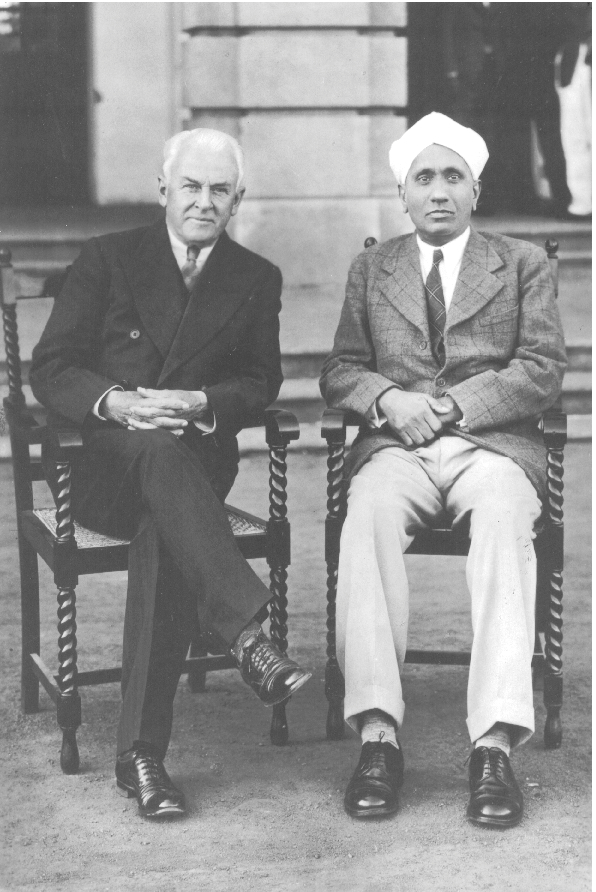
\includegraphics{"images/4.jpg"}
\caption{\enginline{1940}ನೆ ಇಸವಿಯಲ್ಲಿ ಸಿ. ವಿ. ರಾಮನ್‍ರವರೊಡನೆ ಆರ್. ಎ. ಮಿಲ್ಲಿಕನ್. (ಫೋಟೋ ಕೃಪೆ: ಕ್ಯಾಲಿಫೋರ್ನಿಯಾ ಇನ್ಸ್ಟಿಟ್ಯೂಟ್ ಆಫ್ ಟೆಕ್ನಾಲಜಿ, ಆರ್ಖೈವ್ಸ್ ಕ್ಯಾಲಿಫೋರ್ನಿಯಾ ಪಸಾಡೆನಾ).}
\end{figure}

\textbf{ಪಸಾಡೆನಾ ಸ್ಟಾರ್ ನ್ಯೂಸ್} ಎಂಬ ಸ್ಥಳೀಯ ಪತ್ರಿಕೆಯಲ್ಲಿ ಕ್ಯಾಲಿಫೋರ್ನಿಯಾ ಇನ್ಸ್ಟಿಟ್ಯೂಟ್‍ನಲ್ಲಿ ನೀಡಿದ ಉಪನ್ಯಾಸಗಳ ಬಗ್ಗೆ ವರದಿಗಳು ಬಂದವು. ಅದರಲ್ಲಿ ರಾಮನ್ನರ ಉಪನ್ಯಾಸಗಳು ಪಾಮರರೂ ಅರ್ಥ ಮಾಡಿಕೊಳ್ಳುವಷ್ಟು ಸರಳವಾಗಿದ್ದವೆಂದು ಹೊಗಳಲಾಗಿತ್ತು. ರಾಮನ್‍ರವರ ಹಾಸ್ಯ ಪ್ರಜ್ಞೆಯನ್ನೂ, ವಿಷಯದ ಮೇಲಿನ ಹಿಡಿತವನ್ನೂ, ಸ್ವಷ್ಟತೆಯನ್ನೂ ಪ್ರತ್ಯೇಕವಾಗಿ ಪ್ರಶಂಸಿಸಲಾಗಿತ್ತು.

\enginline{1924} ನವೆಂಬರ್ \enginline{18}ರ ಸಂಜೆ, ಯೂನಿವರ್ಸಿಟಿ ಕ್ಲಬ್‍ನಲ್ಲಿ ನೀಡಿದ ಭಾಷಣದ ಬಗ್ಗೆ,\break ಮಾರನೇ ದಿನದ ಪತ್ರಿಕೆಯಲ್ಲಿ “ಭಾರತದ ಸುಪ್ರಸಿದ್ಧ ವಿದ್ವಾಂಸರಿಂದ ಭಾಷಣ” ಎಂಬ ಶೀರ್ಷಿಕೆಯಡಿ ಪ್ರಕಟವಾಯಿತು. ‘\textit{\general{\enginline{A Game of chance}}}’ ಎಂಬುದು ರಾಮನ್ ಅವರಿಗೆ ನೀಡಿದ ವಿಷಯ. ಕಲ್ಕತ್ತ ಯೂನಿವರ್ಸಿಟಿಯಲ್ಲಿ ಥರ್ಮೋಡೈನಾಮಿಕ್ಸ್ ಫ್ರೊಫೆಸರ್ ಆಗಿರುವ ರಾಮನ್‍ರವರು ಇಡೀ ಏಷ್ಯದಲ್ಲಿಯೇ ಶ್ರೇಷ್ಠ ವಿಜ್ಞಾನಿಗಳು. ಅವರು ಪಸಾಡೆನಾದಲ್ಲಿನ ಕ್ಯಾಲಿಫೋರ್ನಿಯಾ ಇನ್ಸ್ಟಿಟ್ಯೂಟ್ ನಲ್ಲಿ ವಿಶೇಷ ಉಪನ್ಯಾಸಗಳನ್ನು ನೀಡುತ್ತಿದ್ದಾರೆ.” ಎಂದು ವರದಿ ಮಾಡಿತು.

ಪೂರ್ವ ದೇಶದಿಂದ ಬಂದ ವಿದ್ವಾಂಸರೊಬ್ಬರು ತಮ್ಮ ಕೇಂದ್ರಕ್ಕೆ ಬಂದಿರುವುದು ವಿಶೇಷವೆಂದು ಯೂನಿವರ್ಸಿಟಿ ಕ್ಲಬ್‍ನ ಅಧ್ಯಕ್ಷರಾಗಿದ್ದ ಕ್ಲಿಂಟನ್ ಕೆ. ಜೂಡಿ ರಾಮನ್‍ರವರನ್ನು ಪರಿಚಯ ಮಾಡಿಕೊಡುವಾಗ ಉದ್ಗರಿಸಿದರು. “ನಮ್ಮ ದೇಶಕ್ಕೆ ಬರುವ ಹಿಂದೂಗಳು ಒಂದೋ ತತ್ತ್ವಜ್ಞಾನದ ಬಗ್ಗೆ ಮಾತನಾಡುತ್ತಾರೆ ಅಥವಾ ಮಂತ್ರ\enginline{-}ತಂತ್ರಗಳ ಬಗ್ಗೆ ಭಾಷಣವೀಯುತ್ತಾರೆ. ಆದರೆ ಇಲ್ಲೊಂದು ಅಪವಾದವಿದೆ. ಪಾಶ್ಚಾತ್ಯ ವಿದ್ವತ್ ಪರಂಪರೆಯನ್ನು ಅರಗಿಸಿಕೊಂಡವರು ಇವರು”. ಎಂದರು ಪ್ರೊಫೆಸರ್ ಜೂಡಿ.

ಡಾ।। ರಾಮನ್‍ರವರು ಸಹ ಬಹಳ ಉತ್ತಮ ವಾಗ್ಮಿತೆ ಪ್ರದರ್ಶಿಸಿದರು. ಅಲ್ಲಲ್ಲಿ ಹಾಸ್ಯಲೇಪವೂ ಇರುತ್ತಿತ್ತು. ಮಾನವನ ಮನಸ್ಸಿಗೆ ಯಾದೃಚ್ಛಿಕವಾಗಿ ನಡೆಯುವ ಆಟ\enginline{-}ಪಾಟಗಳು ಎಂದೆಂದಿಗೂ ಆಸಕ್ತಿಯ ವಿಷಯಗಳಾಗಿವೆ. ಪುರಾತನ ಸಂಸ್ಕೃತ ವಾಙ್ಞಯದಲ್ಲಿ ಮಾನವರು ದೇವತೆಗಳೊಡನೆ ಜೂಜಾಡುವ ಕಥೆಗಳನ್ನು ನೆನಪಿಸಿಕೊಂಡರು.

ಯಾದೃಚ್ಛಿಕವಾಗಿ ನಡೆಯುವ ಆಟಗಳು ಮತ್ತು ನಿತ್ಯ ಜೀವನದ ವಿದ್ಯಮಾನಗಳ ನಡುವೆ ಅಂತಹುದೇನೂ ವ್ಯತ್ಯಾಸವಿಲ್ಲವೆಂದು ರಾಮನ್ ಹೇಳಿದರು. ಯಾದೃಚ್ಛಿಕವಾಗಿ ಏನೂ ನಡೆಯುವುದಿಲ್ಲ ಎಲ್ಲವೂ ಕಾರ್ಯಕಾರಣ ಸಂಬಂಧದಿಂದ ಮಾತ್ರ ಆಗುವಂತಹವು. ಯಾವುದಕ್ಕೆ ನಿರ್ದಿಷ್ಟ ಕಾರಣಗಳು ವೇದ್ಯವಾಗುದಿಲ್ಲವೋ ಅವನ್ನು ಯಾದೃಚ್ಛಿಕ ಎನ್ನುತ್ತಾರೆಂದು ಹೇಳಿದರು.

ಸಂಭವನೀಯತೆಯ ಬಗ್ಗೆ ಪ್ರಸಿದ್ಧ ಗಣಿತಜ್ಞರು ಮಾಡಿದ ಪ್ರಯೋಗಗಳನ್ನು ರಾಮನ್ ನೆನಪಿಸಿದರು. ಯೂನಿವರ್ಸಿಟಿ ಕ್ಲಬ್‍ನ ಸದಸ್ಯರುಗಳೂ ಸಹ ತಮ್ಮ ಕಾಲೇಜು ದಿನಗಳಲ್ಲಿ ಮಾಡಿರಬಹುದಾದ ಜೂಜಾಟಗಳಲ್ಲಿ ಸಂಭವನೀಯತೆ, ಯಾದೃಚ್ಛಿಕತೆ ಹಾಗೂ ಆಯ್ಕೆಗಳ ಬಗ್ಗೆ ಗಮನಿಸಿರಬಹುದೆಂದು ಜ್ಞಾಪಿಸಿದರು. ವಿಪರ್ಯಯ (\enginline{Irreversibility}) ನಿಯಮದ ಬಗ್ಗೆ ಯಾರೂ ಸಹ ಯೋಚಿಸುವುದಿಲ್ಲವೆಂದು ಅವರು ಹೇಳಿದ್ದು ಕುತೂಹಲಕರ ವಿಷಯವಾಗಿತ್ತು.

ಈ ಭಾಷಣವು ಬೌದ್ಧಿಕ ಕಸರತ್ತಿನಂತಾಗಿತ್ತು. “ಅತಿ ದೊಡ್ಡ ಯಾದೃಚ್ಛಿಕತೆ ಇರುವುದು ಪ್ರಕೃತಿಯಲ್ಲಿ” ಎಂದು ಹೇಳಿ ಸಭಿಕರನ್ನು ಉನ್ನತ ಆಲೋಚನೆಗೆ ಕೊಂಡೊಯ್ದರು. ಪಸಾಡೆನಾ ಸ್ಟಾರ್ ನ್ಯೂಸ್ ಪತ್ರಿಕೆಯು \enginline{19} ಡಿಸೆಂಬರ್ \enginline{1924}ರಲ್ಲಿ ರಾಮನ್‍ರವರ ಇನ್ನೊಂದು ಉಪನ್ಯಾಸದ ಬಗ್ಗೆ ವಿವರ ಪ್ರಕಟಿಸಿತು. “ಬೆಳಕಿನ ಸಿದ್ಧಾಂತಗಳು ಎಂಬ ವಿಷಯದ ಬಗ್ಗೆ ಡಾ|| ರಾಮನ್‍ರವರ ಉದ್ಭೋಧಕ ಉಪನ್ಯಾಸ ಪ್ರಾತ್ಯಕ್ಷಿಕೆಗಳ ಜೊತೆಗೆ” ಎಂಬ ಶೀರ್ಷಿಕೆ ನೀಡಿತ್ತು. ಅದರಲ್ಲಿ \enginline{-} “ಕಲ್ಕತ್ತ ಯೂನಿರ್ವಸಿಟಿಯಲ್ಲಿ ಭೌತಶಾಸ್ತ್ರದ ಪ್ರಾಧ್ಯಾಪಕರಾದ ಡಾ|| ಸಿ. ವಿ. ರಾಮನ್‍ರವರು ‘ಬೆಳಕಿನ ಚದರುವಿಕೆ ಮತ್ತು ಅಣು ಮತ್ತು ಪರಮಾಣುಗಳ ವಿನ್ಯಾಸಕ್ಕೆ ಅದರ ಸಂಬಂಧಗಳು’ ಎಂಬ ವಿಷಯದ ಬಗ್ಗೆ ಕ್ಯಾಲಿಫೊರ್ನಿಯಾ ಇನ್ಸ್ಟಿಟ್ಯೂಟ್ ಆಫ್ ಟೆಕ್ನೋಲಜಿಯಲ್ಲಿ ಸೇರಿದ \enginline{300} ಕ್ಕೂ ಹೆಚ್ಚು ಉಪಾಧ್ಯಾಯರು, ವಿದ್ಯಾರ್ಥಿಗಳು ಮತ್ತು ಪದವೀಧರರನ್ನು ಉದ್ದೇಶಿಸಿ ಮಾತನಾಡಿದರು.

ಟೊರಂಟೋ ನಗರದಿಂದ ಸೌಥ್‍ಲ್ಯಾಂಡ್‍ಗೆ ಆಗಮಿಸಿರುವ ಈ ಪ್ರಸಿದ್ಧ ವಿಜ್ಞಾನಿಗಳು ಭಾರತದವರಾಗಿದ್ದು ಇಲ್ಲಿನ ಸಭಿಕರಿಂದ ಅಧಿಕ ಪ್ರಶಂಸೆಯನ್ನು ಗಳಿಸಿದರು.

\vskip 1pt

ರಾಮನ್‍ರವರು ಭೌತಶಾಸ್ತ್ರಜ್ಞರೂ ಹೌದು ಮತ್ತು ರಸಾಯನ ಶಾಸ್ತ್ರಜ್ಞರೂ ಹೌದು. ಇವೆರಡೂ ಶಾಸ್ತ್ರಗಳ ನಡುವಿನ ವಿಷಯಗಳ ಬಗ್ಗೆ ದ್ಯುತಿ ಶಾಸ್ತ್ರವು ಪ್ರವೇಶ ಪಡೆಯುತ್ತದೆ. ಅಣುಗಳ ನಡುವಿನ ವಿನ್ಯಾಸಗಳ ಬಗ್ಗೆ ಬೆಳಕು ಚೆಲ್ಲುತ್ತದೆ. ಇವೆರಡೂ ಶಾಸ್ತ್ರಗಳ ಬಗ್ಗೆ ಅವರು ಆಲೋಚಿಸಿ ಎರಡನ್ನು ಸನಿಹಕ್ಕೆ ತರುವುದೇ ತಮ್ಮ ವೈಜ್ಞಾನಿಕ ಕಾರ್ಯವಾಗಿದೆಯೆಂದು ರಾಮನ್ ಹೇಳಿದರು.

\vskip 1pt

ತಮ್ಮದೇ ಆದ ಬೆಳಕಿನ ಚದರುವಿಕೆಯ ಸಿದ್ಧಾಂತವನ್ನು ರಾಮನ್‍ರವರು ಮಧ್ಯಪ್ರಾಚ್ಯದ ಸಮುದ್ರಯಾನದಲ್ಲಿ ರೂಪಿಸಿದರು. ಸಾಗರದ ಬಣ್ಣ ನೀಲಿ ಏಕೆಂದು ಅವರಿಗೆ ಸಮಸ್ಯೆ ಕಾಡಿತು. ಅವರ ತೃಪ್ತಿಗಾಗಿ ಈ ಸಮಸ್ಯೆಗೆ ಪರಿಹಾರ ಕಂಡುಕೊಂಡರು. ಸೂರ್ಯನ ಬೆಳಕು, ಅಣುಗಳಿಂದ ಚದರಿ ಹೀಗಾಗುತ್ತದೆಂದು ನೂರಾರು ಪ್ರಯೋಗಗಳ ಮೂಲಕ ಸಾಬೀತು ಪಡಿಸಿದರು.

\vskip 1pt

ಅವರ ಉಪನ್ಯಾಸದಲ್ಲಿ ಅನೇಕ ಸರಳ ಪ್ರಯೋಗಗಳಿದ್ದವು. ಅಲ್ಲಿ ನೆರೆದಿದ್ದ ವಿಜ್ಞಾನವೇತ್ತರಿಗಿಂತಲೂ ಪಾಮರರಾದವರಿಗೂ ಅರ್ಥವಾಗಬಲ್ಲ ಪ್ರಯೋಗಗಳಾಗಿದ್ದವು.

\vskip 1pt

ಅವರು ತಂದಿದ್ದ ಒಂದು ಪ್ರಯೋಗದ ಉಪಕರಣವು ಏಳು ಅಡಿ ಉದ್ದವಿತ್ತು. ಅದರಲ್ಲಿ ಪ್ರಯೋಗ ನಿರತರು ತೂರಿ ಕುಳಿತುಕೊಳ್ಳಬಹುದಾಗಿತ್ತು. ರಾಮನ್‍ರವರು ಇದನ್ನು ಕಲ್ಕತ್ತದ ಕಪ್ಪುರಂಧ್ರ ಎಂದು ತಮಾಷೆಯಾಗಿ ಹೇಳಿದರು. (\enginline{Blackhole of Culcutta} ಒಂದು ದುರಂತ ಘಟನೆ. ಸುಮಾರು \enginline{300 – 400} ಜನ ಬಿಳಿಯರನ್ನು ಒಂದು ಸಣ್ಣರೂಮಿನಲ್ಲಿ ಕೂಡಿಹಾಕಿದ್ದರಂತೆ. ಅಲ್ಲಿ ಜನ ಉಸಿರಾಡಲಾಗದೆ ಹುಚ್ಚೆದ್ದು ಹೋಗಿ ಸತ್ತರಂತೆ).

\vskip 1pt

ಒಂದು ಪ್ರಾತ್ಯಕ್ಷಿಕೆಯಲ್ಲಿ ಮುಳುಗುವ ಸೂರ್ಯನ ವರ್ಣ ದೃಶ್ಯ ತೋರಿಸಿದರು. ಒಂದು ಚೌಕಾಕಾರದ ಬಾಟಲಿಯಲ್ಲಿ ದ್ರವವನ್ನು ತುಂಬಿ ಅದರ ಮೂಲಕ ಬೆಳಕು ಹಾಯಿಸಿದ್ದರು (ಇದೇ ಮುಳುಗುವ ಸೂರ್ಯವಾಗಿತ್ತು). ಇದಕ್ಕೆ ಯಾವುದೇ ಸ್ಲೈಡ್ ಬಳಸಿರಲಿಲ್ಲ.

\vskip 1pt

ದಕ್ಷಿಣ ಭಾರತದಲ್ಲಿನ ಮದರಾಸ ಯೂನಿವರ್ಸಿಟಿಯಲ್ಲಿ ರಾಮನ್‍ರವರು ಓದಿದವರು. ವಿಜ್ಞಾನ ಪ್ರಪಂಚದಲ್ಲಿ ಇವರು ಪ್ರಖ್ಯಾತ ಪ್ರಾಧ್ಯಾಪಕರು. ಇದೇ ಮೊದಲ ಬಾರಿಗೆ ಅಮೆರಿಕಾಗೆ, ಹಾಗೂ ಕ್ಯಾಲಿಫೊರ್ನಿಯಾಗೆ ಬಂದಿದ್ದಾರೆ. ನಮ್ಮ ಸೌಥ್ ಲ್ಯಾಂಡ್ ಬಗ್ಗೆ ತೀವ್ರ ಆಸಕ್ತಿಯನ್ನು ವ್ಯಕ್ತಪಡಿಸಿದರು. ಇಲ್ಲಿರುವವರ ದ್ಯುತಿ ಪ್ರಯೋಗಗಳ ಬಗೆಗಿನ ಆಸಕ್ತಿಯನ್ನು ನೋಡಿ ಆಶ್ಚರ್ಯಗೊಂಡರು. ಭಾರತದಲ್ಲಿ ವಿಜ್ಞಾನ ಉಪನ್ಯಾಸಗಳಿಗೆ ಇಂತಹ ಪ್ರೋತ್ಸಾಹವಿಲ್ಲವೆಂದು ಖೇದ ವ್ಯಕ್ತಪಡಿಸಿದರು.

\vskip 1pt

ರಾಮನ್‍ರವರು ಪಸಾಡೆನಾಗೆ ಬಂದದ್ದರಿಂದ ಅಮೆರಿಕಾದ ಪ್ರಸಿದ್ಧ ವಿಜ್ಞಾನಿಗಳ ಪರಿಚಯವಾಯಿತು. ಹಾಗೆಯೇ ಆರ್. ಎ. ಮಿಲ್ಲಿಕನ್ ಅವರ ಜೊತೆಗೆ ಜೀವನ ಪರ್ಯಂತ ಸ್ನೇಹ ಸಂಪಾದಿಸಿದರು. ಮಿಲ್ಲಿಕನ್ ಅವರ ಬಗ್ಗೆ ರಾಮನ್‍ರವರ ಮೆಚ್ಚುಗೆಯನ್ನು ಕ್ಯಾಲಿಫೊರ್ನಿಯಾ ಇನ್ಸ್ಟಿಟ್ಯೂಟ್ ಆಫ್ ಟೆಕ್ನೋಲಜಿಯಲ್ಲಿನ ಉಪನ್ಯಾಸದ ವೇಳೆಗೆ ಮಾಡಿದ ಪ್ರಕಟಣೆಯೊಂದು ತಿಳಿಸುತ್ತದೆ. ಇದನ್ನು ತಯಾರಿಸಿದವರು ಮಿಲ್ಲಿಕನ್ ಅವರೇ. ಇದು \enginline{1924}ರ ಡಿಸೆಂಬರ್ \enginline{9} ರಂದು ಪ್ರಕಟಗೊಂಡಿತು.

“ಕ್ಯಾಲಿಫೋರ್ನಿಯಾ ಇನ್ಸ್ಟಿಟ್ಯೂಟ್‍ನಲ್ಲಿ ಶುಕ್ರವಾರದ ಸಂಜೆಯ ಉಪನ್ಯಾಸವು ಅತಿ ವಿಶೇಷದ್ದು. ಏಕೆಂದರೆ ಉಪನ್ಯಾಸ ನೀಡಲಿರುವ ಕಲ್ಕತ್ತ ಯೂನಿವರ್ಸಿಟಿಯ ಪ್ರಾಧ್ಯಾಪಕರಾದ ರಾಮನ್‍ರವರದ್ದು ವಿಶೇಷ ವ್ಯಕ್ತಿತ್ವ. ಅಲ್ಲದೆ ಅವರು ಮಂಡಿಸುವ “ಸಂಗೀತ ವಾದ್ಯಗಳ ಅಧ್ಯಯನ ವಿಷಯವು” ಮತ್ತೂ ವಿಶೇಷವಾದದ್ದು.

ಪೂರ್ವ ದೇಶಗಳಲ್ಲಿ ರಾಮನ್‍ರವರು ಅತಿಹೆಚ್ಚು ಸಂಶೋಧನೆಗಳನ್ನು ಮಾಡಿರುವ ವ್ಯಕ್ತಿಯಾಗಿ ಪ್ರತ್ಯೇಕ ಸ್ಥಾನ ಹೊಂದಿದ್ದಾರೆ. ಅವರು ಮಾಡಿರುವ ವಿಶಿಷ್ಠ ಅಧ್ಯಯನಗಳೇ ಅಲ್ಲದೆ ಅವರು ಹಲವಾರು ವಿದ್ಯಾರ್ಥಿಗಳನ್ನು ಸಂಶೋಧನೆಗಳಿಗೆ ತೊಡಗಿಸಿದ್ದಾರೆ. ತಂತಿ ವಾದ್ಯಗಳ ಮೇಲಿನ ಅವರ ಸಂಶೊಧನೆಗಳು ಅವರಿಗೆ ಅಂತಾರಾಷ್ಟ್ರೀಯ ಖ್ಯಾತಿ ತಂದುಕೊಟ್ಟಿದೆ. ಇದರ ಬಗ್ಗೆಯೇ ಅವರು ಇಲ್ಲಿ ವಿಚಾರ ಮಂಡಿಸುತ್ತಿದ್ದಾರೆ. ಈ ವಿಷಯವೇ ಅತಿ ವಿಶಿಷ್ಟವಾದರೂ, ರಾಮನ್‍ರವರ ವಾಗ್ಮಿತೆಯು ಪ್ರಶಂಸನೀಯವಾದುದು, ಅವರ ಭಾಷಣದ ಆಳ, ಹರಹುಗಳು ಅತ್ಯಾಕರ್ಷಕ. ಅವರ ವಿಷಯ ಮಂಡನೆಯ ರೀತಿ ಅತಿವಿಶೇಷವಾಗಿರುತ್ತದೆ. ವಿಷಯ ಜ್ಞಾನ ಮತ್ತು ಅವರ ಇಂಗ್ಲಿಷ್ ಭಾಷೆಯ ಮೇಲಿನ ಪ್ರಭುತ್ವಗಳು ಚೇತೋಹಾರಿಯಾಗಿರುತ್ತವೆ. ಅವರು ಈ ಚಳಿಗಾಲದಲ್ಲಿ ಥರ್ಮೋಡೈನಾಮಿಕ್ಸ್ ಬಗ್ಗೆ ಉಪನ್ಯಾಸ ಸರಣಿ ನೀಡಲು ಬಂದವರಾದರೂ, ಜನಪ್ರಿಯ ವಿಜ್ಞಾನ ಉಪನ್ಯಾಸಕ್ಕಾಗಿ ತಂತಿ ವಾದ್ಯಗಳ ಮೇಲಿನ ಅನೇಕ ವಿಶೇಷ ಪ್ರಾತ್ಯಕ್ಷಿಕೆಗಳನ್ನೂ ನೀಡಲಿದ್ದಾರೆ.”

ಈ ಉಪನ್ಯಾಸವು ಸಂಜೆ \enginline{7} ರಿಂದ \enginline{8} ಗಂಟೆಯವರೆಗೆ “ನಾರ್ಮನ್ ಬ್ರಿಡ್ಜ್ ಲ್ಯಾಬೊರೇಟರಿ ಹಾಲ್ ನಲ್ಲಿ ನಡೆಯಲಿದೆ. ಇದು ಸಾರ್ವಜನಿಕರಿಗೆ ಮುಕ್ತವಾಗಿದ್ದು ಯಾವುದೇ ಶುಲ್ಕವಿರುವುದಿಲ್ಲ”. ರಾಮನ್‍ರವರು \enginline{1925}ರ ಫೆಬ್ರವರಿಯಲ್ಲಿ ಅನೇಕ ದೇಶಗಳ ಮೂಲಕ ಸಾಗಿ ಸ್ವದೇಶಕ್ಕೆ ಮರಳಿದರು. ಈ ದೇಶಗಳಲ್ಲಿ ಆಗಿನ ಕಾಲದ ಪ್ರಸಿದ್ಧ ವಿಜ್ಞಾನಿಗಳಾದ ನೀಲ್ಸ್ ಬೋರ್, ಮಾಕ್ಸ್ ಪ್ಲಾಂಕ್, ಫೆಬ್ರೀ, ಸೀಗ್ ಬಾಹನ್ ಮುಂತಾದವರನ್ನು ಭೇಟಿಯಾದರು.

ರಾಮನ್‍ರವರ ವಿದೇಶ ಪ್ರಯಾಣಗಳೂ ಮತ್ತು ಹಿರಿಯ ವಿಜ್ಞಾನಿಗಳೊಡನೆ ಸಂಪರ್ಕವೂ ಅವರ ಕಾರ್ಯದ ಮೇಲೂ ಹವ್ಯಾಸಗಳ ಮೇಲೂ ದೊಡ್ಡ ಪರಿಣಾಮ ಬೀರಿತು. ಮೊದಲಿಗೆ ರಾಮನ್‍ರವರು ಹಗಲು ರಾತ್ರಿಯೆನ್ನದೆ ಕಾರ್ಯಮಗ್ನರಾಗುತ್ತಿದ್ದರು. ಒಮ್ಮೆ ಕೆಲಸ ಶುರು ಮಾಡಿದರೆಂದರೆ ಒಮ್ಮೆಗೇ ಕುಳಿತು ಬಿಡುತ್ತಿದ್ದರು. ಊಟ, ತಿಂಡಿ, ನಿದ್ರೆಗಳ ಪರಿವೆಯೇ ಇರಲಿಲ್ಲ. ಇವರ ವಿದೇಶಿ ಪ್ರಯಾಣದ ಬಳಿಕ ಇವೆಲ್ಲವೂ ಮಾರ್ಪಾಡಾದವು. ಅವರು ಹೆಚ್ಚು ವ್ಯವಸ್ಥಿತವಾಗಿಯೂ, ನಿಯಮಿತವಾಗಿಯೂ ಕೆಲಸ ಮಾಡತೊಡಗಿದರು. ಅವರ ಶಿಷ್ಯರಿಗೆ ಕೆಲಸ ಹಂಚುವಾಗಲೂ, ಅವರು ಸಂಶೋಧನೆಗೆ ತೊಡಗಿಸಿಕೊಳ್ಳುವಾಗಲೂ ಹೆಚ್ಚು ವೃತ್ತಿಪರತೆ ತಂದುಕೊಂಡರು. ಸರಿಯಾದ ಕಾಲಕ್ಕೆ ತಿಂಡಿ ತೀರ್ಥಗಳೂ ಆಗಾಗ ವಿರಾಮಕ್ಕೆ ಸಮಯ ತೆಗೆದುಕೊಳ್ಳುವುದೂ ಶ‍್ರೀಮತಿ ರಾಮನ್ ಅವರಿಗೆ ಆಪ್ಯಾಯಮಾನವಾಗಿ ಕಂಡಿರಬಹುದು. 

ರಾಮನ್‍ರವರು \enginline{FRS} ಪಡೆದ ಮೇಲೆ ಕಲ್ಕತ್ತ ಯೂನಿವರ್ಸಿಟಿಯವರು ಅವರ ವೇತನ ಹೆಚ್ಚಿಸಿದರು. ಇದರಿಂದಾಗಿ ಎಲ್.ಎ.ರಾಮದಾಸ್ ಅವರು ಹೇಳುವಂತೆ, ರಾಮನ್‍ರವರು ಒಂದು ಕುದುರೆಗಾಡಿಯನ್ನು \enginline{1924}ರಲ್ಲಿ ಕೊಂಡರಂತೆ. ಅದರ ಪಾಲಕನೂ, ಗಾಡಿ ಓಡಿಸುವವನೂ ಒಬ್ಬನೇ ಆಗಿದ್ದನಂತೆ. ಹೀಗಾಗಿ ಟ್ಯಾಕ್ಸಿಯ ಮೇಲೆ ರಾಮನ್‍ರವರ ಅವಲಂಬನೆ ಇಲ್ಲವಾಯಿತು. ಕಂದು ಬಣ್ಣದ ಕುದುರೆ ಕರಿಬಣ್ಣದ ಗಾಡಿ ನೋಡಲು ಭರ್ಜರಿಯಾಗಿದ್ದವಂತೆ. ಇದರಲ್ಲಿ ಸಾಯಂಕಾಲದ ವಿಹಾರಗಳಲ್ಲಿ ಜೊತೆಗೆ ಶ‍್ರೀಮತಿ ರಾಮನ್‍ರವರು ಇರದಿದ್ದಾಗ ಯಾರಾದರೂ ಸಂಶೋಧಕ ಮಿತ್ರರನ್ನು ಕರೆದುಕೊಂಡು ಹೋಗುತ್ತಿದ್ದರಂತೆ. 

ರಾಮನ್‍ರವರ ಜೊತೆಗೆ ಸಹಪಯಣವನ್ನು ರಾಮದಾಸ್ ಅವರು ಹೀಗೆ ವಿವರಿಸುತ್ತಾರೆ \enginline{-} “ಸಂಜೆಯ ವಿಹಾರವು ಕಲ್ಕತ್ತ ಮೈದಾನದ ಕಡೆಗೆ ಹೊರಡುತ್ತಿತ್ತು. ಅದು ಲಾರ್ಡ್ ಕಿಚ್ನರ್ ಅಥವಾ ಲಾರ್ಡ್ ರೋಬರ್ಟ್ರವರ ಪುತ್ಥಳಿಗಳ ಬಳಿ ನಿಲ್ಲುತ್ತಿತ್ತು. ರಾಮನ್‍ರವರು ಫೋರ್ಟ್ ವಿಲಿಯಂನ ಕಡೆಗೆ ಗಡಿಬಿಡಿಯಿಂದ ನಡೆಯುತ್ತಿದ್ದರು. ಬಳಿಕ ದಂಡಹಾಕಿ ಕಸರತ್ತು ಮಾಡುತ್ತಿದ್ದರು. ಅಲ್ಲಿಂದ ವಾಪಸ್ ಮನೆಗೆ. ಒಮ್ಮೆ ಹೀಗೆ ಗಾಡಿಯ ಕಡೆ ವಾಪಸ್ ಹೆಜ್ಜೆಹಾಕುತ್ತಿದ್ದಾಗ ಅರ್ಧ ಮೈಲಿ ಸಾಗಿದ ನಂತರ ಈಗ ವೇಳೆಯೆಷ್ಟು ಎಂದು ಕೇಳಿದರು. ನಾನು \enginline{7.20} ಎಂದೆ. ನಿನ್ನ ಬಳಿ ವಾಚ್ ಇದೆಯೇ ಎಂದರು. ನಾನು ದೂರದ ಗೋಪುರದ ವೈಟ್ ವೇ ಮತ್ತು ಲಿಡ್ಲಾ ಗಡಿಯಾರ ತೋರಿಸಿದೆ. ಅವರು ಈ ನಡಿಗೆಯು ಸರಿಯಾಗಿ \enginline{12} ನಿಮಿಷಗಳಾಗುತ್ತವೆಂದೂ ನಾನದನ್ನು ಲೆಕ್ಕವಿಡಬೇಕೆಂದು ಹೇಳಿದರು. ಅವರು ಗಾಡಿಯ ಬಳಿಗೆ ಬಂದಾಗ ಸರಿಯಾಗಿ \enginline{7.32} ಆಗಿತ್ತು. ನಾನು ನಿಟ್ಟುಸಿರು ಬಿಟ್ಟೆ. ನನ್ನ ಕಣ್ಣಿನ ದೂರದೃಷ್ಟಿಯ ಬಗ್ಗೆ ಅವರು ಮೆಚ್ಚುಗೆ ಸೂಚಿಸಿದರು. ಗಾಡಿಯಲ್ಲಿ ವಾಪಸಾಗುವಾಗ ನಮ್ಮ ಸಂಶೋಧನೆಗಳ ಬಗ್ಗೆ ಬಹಳ ಚರ್ಚಿಸಿದೆವು. ಅನೇಕ ಹೊಸ ಮಾರ್ಗಗಳು ಹೊಳೆದವು. ಸಮಯ ಕಳೆದಿದ್ದೆ ಗೊತ್ತಾಗಲಿಲ್ಲ. ಅಸೋಸಿಯೇಷನ್ ಬಳಿಯಲ್ಲಿಯೇ ನನ್ನ ಮನೆಯೂ ಇತ್ತು. ಒಳಗೆ ನುಗ್ಗಿ ಹಿಂಬದಿಯ ಗೇಟಿನಿಂದ ತೂರಿ ಮನೆಗಳನ್ನು ತಲುಪಿದೆವು. ಹಿಂಬಾಗಿಲ ಕೀಲಿ ಹಿಡಿದ ಕೆಲವೇ ಮಂದಿಯಲ್ಲಿ ನಾನು ಒಬ್ಬ”.


\heading{ರಾಮನ್ ಎಫೆಕ್ಟ್‌ನ ಆವಿಷ್ಕಾರ}

ರಾಮನ್‍ರವರ ಕೈ ಕೆಳಗೆ ಕೆಲಸಮಾಡುತ್ತಿದ್ದ ಕೆ.ಆರ್.ರಾಮನಾಥನ್ ಅವರು ನೀರಿನಲ್ಲಿ ಬೆಳಕಿನ ಚದರುವಿಕೆಯ ಬಗ್ಗೆ ಕೂಲಂಕಷ ಅಧ್ಯಯನವನ್ನು \enginline{1923}ರಲ್ಲಿ ಕೈಗೆತ್ತಿಕೊಂಡರು. ನೀರನ್ನು ಒಂದು ಬಾಟಲಿಯಲ್ಲಿಟ್ಟು ಸೂರ್ಯನ ಬೆಳಕನ್ನು ಅದರ ಮೂಲಕ ಹಾಯಿಸಿ ಇದಕ್ಕೆ ಲಂಬವಾಗಿ ಚದರುವ ಬೆಳಕನ್ನು ವೀಕ್ಷಣೆ ಮಾಡತೊಡಗಿದರು. ಪರಸ್ಪರ ಹೊಂದಾಣಿಕೆಯಾಗಬಲ್ಲ ಸೋಸುಕಗಳನ್ನು ಬಳಸಿ ಹಾಯುವ ಬೆಳಕಿನ ತೀವ್ರತೆಯನ್ನು ದಾಖಲಿಸತೊಡಗಿದರು. ಲಂಬವಾಗಿ ಚದರುವ ಬೆಳಕನ್ನು ಕ್ಷೀಣ ದೀಪ್ತಿ (\enginline{Luminescence}) ಎಂದು ಗುರುತಿಸಿದ್ದರು. ಇದು ದ್ರವದಲ್ಲಿ ಇರಬಹುದಾದ ಅಶುದ್ಧ ಕಣಗಳಿಂದ ಆಗಿರಬಹುದೆಂದು ತರ್ಕಿಸಿದ್ದರು. ಆದರೆ ಹಲವಾರು ಬಾರಿ ದ್ರವವನ್ನು ಬಾಷ್ಪೀಕರಣದಿಂದ ಶುದ್ಧಿ ಮಾಡಿದ ನಂತರವೂ ಈ ಕ್ಷೀಣ ದೀಪ್ತಿಯು ಹಾಗೆಯೇ ಉಳಿಯಿತು. ರಾಮನ್ ಅವರಿಗೆ ಈ ಪ್ರಯೋಗವು ಸಮರ್ಪಕವಾಗಿ ಕಾಣಲಿಲ್ಲ. ಅವರು ಇದು ಎಕ್ಸ್\enginline{-}ರೇಯೊಳಗೆ ಕಾಂಪ್ಟನ್ ಪರಿಣಾಮವಿದ್ದಂತೆ, ಸಾಮಾನ್ಯ ಬೆಳಕಿನಲ್ಲಿ ಇದೇ ಮಾದರಿಯ ವಿದ್ಯಮಾನವಿರಬಹುದು ಎಂದು ಊಹಿಸಿದರು.

ಎರಡು ವರ್ಷಗಳ ತರುವಾಯ ಮಾಡಿದ ಪ್ರಯೋಗಗಳಲ್ಲಿ \enginline{65} ಬಗೆಯ ಶುದ್ಧ ದ್ರವಗಳಲ್ಲಿ ಈ ಬಗೆಯ ದೀಪ್ತಿ ಉಂಟಾಗುವುದು ಕೆ. ಎಸ್. ಕೃಷ್ಣನ್ ಅವರಿಗೆ ಕಾಣಿಸಿತು. ಅವರು ಈ ಚದರಿದ ಬೆಳಕಿನ ಬಗ್ಗೆ ಒಂದು ಮುಖ್ಯ ವಿಷಯವನ್ನು ತಿಳಿದರು. ಅದು ಈ ದೀಪ್ತಿ ಬೆಳಕು ಅಪೂರ್ಣವಾಗಿ ಧ್ರುವೀಕರಣಗೊಳ್ಳುತ್ತಿದೆಯೆಂಬ ಅಂಶ. ಯಾವುದೇ ಸಾಮಾನ್ಯ ದೀಪ್ತಿಯು ಹೀಗಾಗುವುದಿಲ್ಲ ಇವರು ಮಾಡಿದ ಪ್ರಯೋಗಗಳಲ್ಲಿ ಸೂರ್ಯನ ಬೆಳಕನ್ನು ಒಂದು ದೊಡ್ಡ ಮಸೂರದಿಂದ ಒಟ್ಟುಗೂಡಿಸಿ, ದ್ರವ ತುಂಬಿದ ಗಾಜಿನ ಬಾಟಲಿಯ ಮೂಲಕ ಹಾಯಿಸುತ್ತಿದ್ದರು. ದ್ರವದ ಮೂಲಕ ಹಾಯುವ ಬೆಳಕನ್ನು ನೇರಳೆ\enginline{-}ನೀಲಿ ಫಿಲ್ಟರ್‍ಗಳ ಮೂಲಕ ಕಳುಹಿಸುತ್ತಿದ್ದರು. ಚದರಿದ ಬೆಳಕು ಹಸಿರು\enginline{-}ಹಳದಿ ಫಿಲ್ಟರ್‍ಗಳ ಮೂಲಕ ಹಾಯ್ದು ಬರುತ್ತಿತ್ತು.

ಕೆ.ಎಸ್.ಕೃಷ್ಣನ್ ಅವರ ನಂತರ ಬಂದ ಎಸ್.ವೆಂಕಟೇಶ್ವರನ್ ಅವರು \enginline{1925}ರಲ್ಲಿ ಇದೇ ಕೆಲಸವನ್ನು ಮುಂದುವರೆಸಿದರು. ಚದರಿದ ಬೆಳಕಿನ ರೋಹಿತ ಪಟ್ಟಿಯನ್ನು ಫೋಟೋ ಮಾಡಿಕೊಳ್ಳಲು ಪ್ರಯತ್ನಿಸಿದರಾದರೂ, ಅದು ಸೂರ್ಯನ ಬೆಳಕಿನಲ್ಲಿ ಸಾಧ್ಯವಾಗಲಿಲ್ಲ. ಫಿಲ್ಟರ್‍ಗಳ ಮೂಲಕ ಹಾಯ್ದು ಬಂದ ಚದರಿದ ಬೆಳಕಿಗೆ ಫೋಟೋ ಮೂಡಿಸುವಷ್ಟು ತೀವ್ರತೆಯಿರಲಿಲ್ಲ. ಇವೆಲ್ಲ ಪ್ರಯೋಗಗಳೂ ರಾಮನ್‍ರವರ ಮಾರ್ಗದರ್ಶನದಲ್ಲಿಯೇ ನಡೆಯುತ್ತಿದ್ದವು. ಅವರು ಕ್ಷೀಣ ಪ್ರತಿದೀಪ್ತಿಯ ಬೆಳಕನ್ನು ಒಪ್ಪಲಿಲ್ಲ. ರೋಹಿತ ಪಟ್ಟಿಯಲ್ಲಿ ಬೇರೆಯಾಗಿ ಗೆರೆಗಳು ಕಂಡವಾದರೂ ಅವು ಪ್ರತಿದೀಪ್ತಿಯವಲ್ಲ ಎಂಬ ಊಹೆ ಅವರಿಗಿತ್ತು. ಏಕೆಂದರೆ ಪ್ರತಿದೀಪ್ತಿಯ ಬೆಳಕಿನ ತೀವ್ರತೆ ಜಾಸ್ತಿಯಾಗಿರುತ್ತದೆ ಮತ್ತು ಅವು ಧ್ರುವೀಕರಣಗೊಂಡಿರುವುದಿಲ್ಲ. ಇದು ಇನ್ನಾವುದೋ ಬಗೆಯಲ್ಲಿ ಹೊರಸೂಸುವ ಕಿರಣಗಳಿರಬಹುದೆಂದು, ದೀಪ್ತಿಯ ಕಿರಣಗಳಲ್ಲವೆಂದೂ ಅವರು ಊಹಿಸಿದ್ದರು.

\enginline{1927}ರಲ್ಲಿ ಕಾಂಪ್ಟನ್ ಅವರಿಗೆ ಸಂದ ನೊಬೆಲ್ ಪಾರಿತೋಷಕವು ರಾಮನ್ ಅವರಿಗೆ ಬೆಳಕಿನ ಇದೇ ಬಗೆಯ ಪರಿಣಾಮವನ್ನು ಕಂಡುಹಿಡಿಯಲು ಒತ್ತಾಸೆ ನೀಡಿತು. ಕಲ್ಕತ್ತದ ದಿನಗಳಲ್ಲಿ ರಾಮನ್‍ರವರ ಶಿಷ್ಯರಾಗಿದ್ದ ಬಿ. ಎನ್. ಶ‍್ರೀನಿವಾಸಯ್ಯನವರು ಅಸೋಸಿಯೇಷನ್‍ನಲ್ಲಿ ನಡೆದ ಈ ಘಟನೆಗೆ ಸಾಕ್ಷಿಯಾಗಿದ್ದರು. ಅವರು ಹೀಗೆ ಹೇಳುತ್ತಾರೆ\enginline{-}

“\enginline{1927}ರ ನವೆಂಬರ್ ತಿಂಗಳ ಸಂಜೆ ನಾನು ಕಲ್ಕತ್ತದಲ್ಲಿದ್ದೆ. ದೆಹಲಿಯಲ್ಲಿ ಪರೀಕ್ಷೆ ಮತ್ತು ಸಂದರ್ಶನ ಮುಗಿಸಿಕೊಂಡು ರಾಮನ್‍ರವರ ಆಶೀರ್ವಾದ ಪಡೆಯಲು ಅಸೋಸಿಯೇಷನ್ನಿನ ಕಚೇರಿಗೆ ಹೊಕ್ಕೆ. ಆಗ ರಾಮನ್‍ರವರ ಹಿರಿಯ ಅಣ್ಣಂದಿರಾದ ಸುಬ್ರಮಣ್ಯ ಅಯ್ಯರ್ (ನೊಬೆಲ್ ವಿಜೇತ ಚಂದ್ರಶೇಖರ್ ಅವರ ತಂದೆ) ಅಲ್ಲಿದ್ದರು. ನಾನು ಅಲ್ಲಿದ್ದಂತೆಯೇ ಕೆ.ಎಸ್.ಕೃಷ್ಣನ್ ರವರು ಅತ್ಯುತ್ಸಾಹದಿಂದ ಒಳಗೆ ಬಂದರು. ಸಂಜೆಯ ಪತ್ರಿಕೆಗಳಲ್ಲಿ ಎ.ಎಚ್.ಕಾಂಪ್ಟನ್ ರವರಿಗೆ ನೊಬೆಲ್ ಬಹುಮಾನ ಕೊಟ್ಟಿರುವುದನ್ನು ತಿಳಿಸಿದರು. ಅದು ಎಕ್ಸ್\enginline{-}ರೇ ಬಳಸಿದ ಕಾಂಪ್ಟನ್ ಎಫೆಕ್ಟ್ ಆವಿಷ್ಕಾರಕ್ಕೆಂದೂ ಹೇಳಿದರು. ಅದನ್ನು ಕೇಳಿದೊಡನೆಯೇ ರಾಮನ್‍ರವರ ಮುಖ ಅಗಲವಾಯಿತು. ಅವರದೇ ಶೈಲಿಯಲ್ಲಿ “ಎಂತಹ ಅದ್ಭುತ ಸಮಾಚಾರ...... ಬಹಳ ಒಳ್ಳೆಯದಾಯಿತು. ಇಲ್ಲಿ ನೋಡಿ ಕೃಷ್ಣನ್, ಇದು ಎಕ್ಸ್\enginline{-}ರೇಗಳಿಗೆ ನಿಜವಾದದ್ದಾದರೆ, ಬೆಳಕಿಗೂ ನಿಜವೇ ಆಗಬೇಕು. ನಾನು ಇದನ್ನು ಮೊದಲಿನಿಂದಲೂ ಯೋಚಿಸುತ್ತಿದ್ದೇನೆ. ಕಾಂಪ್ಟನ್ ಪರಿಣಾಮಕ್ಕೆ ಗೋಚರ ಬೆಳಕಿನ ಸಾದೃಶ್ಯ ಪರಿಣಾಮವಿರಲೇ ಬೇಕು. ನಾವು ಈಗ ಮಾಡುತ್ತಿರುವ ಪ್ರಯೋಗಗಳು ಈ ನಿಟ್ಟಿನಲ್ಲೇ ಇವೆ. ನಾವಿದನ್ನು ಮುಂದುವರಿಸಬೇಕು. ಇದು ಸಿಕ್ಕೇ ಸಿಗುತ್ತದೆ. ನಾವು ಆವಿಷ್ಕರಿಸಬೇಕು, ನೊಬೆಲ್ ಬಹುಮಾನ ಗೆಲ್ಲಲೇಬೇಕು”.

ಇದಾದ ಕೆಲವು ತಿಂಗಳ ಬಳಿಕ ರಾಮನ್‍ರವರು ಬೆಂಗಳೂರಿನಲ್ಲಿ ನೀಡಿದ “\enginline{\textit{On the New Radiation}}” (ಹೊಸ ಕಿರಣಗಳು) ಉಪನ್ಯಾಸಕ್ಕೂ ಶ‍್ರೀನಿವಾಸಯ್ಯ ಹಾಜರಾಗಿದ್ದರು.

ಕೆಲವು ವರ್ಷಗಳ ಕಾಲ ಈ ಪ್ರಯೋಗಗಳನ್ನು ನಿಲ್ಲಿಸಲಾಗಿತ್ತು. ಏಕೆಂದರೆ ಕೆ. ಎಸ್. ಕೃಷ್ಣನ್ ಅವರು ಸೈದ್ಧಾಂತಿಕ ಗಣಿತೀಯ ಸಮಸ್ಯೆಗಳತ್ತ ತಮ್ಮ ಕಾರ್ಯವನ್ನು ತೊಡಗಿಸಿಕೊಂಡಿದ್ದರು.

\enginline{1927} ರ ಚಳಿಗಾಲದಲ್ಲಿ ರಾಮನ್‍ರವರು ಆಂಧ್ರಪ್ರದೇಶದ ವಾಲ್ಟೇರ್ ನಗರಕ್ಕೆ ವಿಹಾರಕ್ಕಾಗಿ ತೆರಳಿದ್ದರು. ಇದು ಸಮುದ್ರ ತೀರದಲ್ಲಿರುವ ನಗರ. ಅವರ ಮನಸ್ಸಿನಲ್ಲಿ ಕಾಂಪ್ಟನ್ ಪರಿಣಾಮವೇ ತುಂಬಿತ್ತು. ಇದರ ಬಗ್ಗೆಯೇ ಲೆಕ್ಕಾಚಾರ ಮಾಡತೊಡಗಿದರು. ಅವರು ಕಾಂಪ್ಟನ್ ಅವರ ಸಮೀ\-ಕರಣವನ್ನು ಪಡೆದುಕೊಳ್ಳುತ್ತಿದ್ದಂತೆಯೇ ತಾವು ಕಂಡಿದ್ದ ಕ್ಷೀಣ ಪ್ರತಿದೀಪ್ತಿಯಲ್ಲಿ ಕಾಂಪ್ಟನ್\break ಪರಿಣಾಮದಂತೆಯೇ, ಚದರಿದ ಬೆಳಕಿನ ತರಂಗಾಂತರ ಬದಲಾಗಿರಬಹುದೆಂದು ತರ್ಕಿಸಿದರು. ಈ ಹೊಸ ಹೊಳಹನ್ನು ಹೊತ್ತು ತಂದ ರಾಮನ್‍ರವರು ತಮ್ಮ ಹಿಂದಿನ ಪ್ರಯೋಗಗಳ ಸಮಸ್ಯೆಗೆ ಪರಿಹಾರ ಹುಡುಕಲು ತೀವ್ರ ಗಮನ ಹರಿಸಿದರು. ಕೃಷ್ಣನ್ ರವರಿಗೆ ಅವರ ಸೈದ್ಧಾಂತಿಕ ಗಣಿತ ಸಮಸ್ಯೆಗಳ ಕಾರ್ಯವನ್ನು ಸ್ಥಗಿತಗೊಳಿಸಲು ಹೇಳಿ ದ್ರವಗಳು ಮತ್ತು ಅವುಗಳ ಆವಿಯ ಮೂಲಕ ಚದರಿದ ಬೆಳಕಿನ ಅಧ್ಯಯನವನ್ನು ಪ್ರಯೋಗಗಳ ಮೂಲಕ ಇನ್ನಷ್ಟು ನಿಖರವಾಗಿ ಮಾಡಲು ಆದೇಶಿಸಿದರು. ವೆಂಕಟೇಶ್ವರನ್ ಮತ್ತು ಕೃಷ್ಣನ್ ಅವರನ್ನು ದ್ರವಗಳನ್ನು ಶುದ್ಧಿಕರಿಸುವ ಕೆಲಸಕ್ಕೆ ಹಚ್ಚಿದರು. ಈ ಮೊದಲು ಮಾಡಿದ ಪ್ರಯೋಗಗಳನ್ನು ಪುನಃ ಮಾಡುವಂತೆ ತಿಳಿಸಿದರು. ಜನವರಿ \enginline{1928}ರಲ್ಲಿ ವೆಂಕಟೇಶ್ವರನ್ ಅವರು, ಗ್ಲಿಸರಿನ್ ದ್ರವದ ಪ್ರಯೋಗದಲ್ಲಿ ಚದರಿದ ಬೆಳಕು ನೀಲಿ ಬಣ್ಣದಲ್ಲಿಲ್ಲದೆ ಹಸಿರು ಬಣ್ಣದಲ್ಲಿತ್ತೆಂದು ವರದಿ ಮಾಡಿದರು. ಅಲ್ಲದೆ ಈ ಬೆಳಕಿನ ಕಿರಣಗಳು ಧ್ರುವೀಕರಣಗೊಂಡಿದ್ದವು. ಇದು ಪ್ರಯೋಗಗಳನ್ನು ಮುಂದುವರಿಸಲು ಇನ್ನಷ್ಟು ಸಬಲ ಕಾರಣ ನೀಡಿತು.

ಚದರಿದ ಬೆಳಕಿನ ಸಾಂದ್ರತೆಯನ್ನು ಹೆಚ್ಚು ಮಾಡಲು ರಾಮನ್ ಮತ್ತು ಕೃಷ್ಣನ್ ಅವರು ಹೊಸ ಪ್ರಯೋಗ ಉಪಕರಣಗಳನ್ನು ಸಿದ್ಧಪಡಿಸತೊಡಗಿದರು. ಈ \enginline{18}ಸೆ.ಮೀ. ದೂರದರ್ಶಕದಿಂದ ಸೂರ್ಯನ ಬೆಳಕನ್ನು ಹಾಯಿಸಿ, ಅದನ್ನು ಮಸೂರದಿಂದ ಕೇಂದ್ರೀಕರಿಸಲು ಉಪಕರಣಗಳನ್ನು ಜೋಡಿಸಿದರು. ಈ ಬೆಳಕನ್ನು ನೇರಳೆ ಫಿಲ್ಟರ್ ಮೂಲಕ ಹಾಯಿಸಿ, ಅದರ ಮುಂದೆ ಮೊಹರು ಮಾಡಿದ ಗಾಜಿನ ಬಾಟಲಿಯೊಳಗೆ ಪ್ರಯೋಗ ದ್ರವವನ್ನು ಇರಿಸಿದರು. ಈ ದ್ರವವನ್ನು ಹಲವಾರು ಬಾರಿ ನಿರ್ವಾತದಲ್ಲಿ ಬಾಷ್ಪೀಕರಣಗೊಳಿಸಿ ಶುದ್ಧೀಕರಿಸಲಾಗಿತ್ತು. ಮೊದಲು ಇರಿಸಿದ ನೀಲಿ\enginline{-}ನೇರಳೆ ಫಿಲ್ಟರಿಗೆ ಪೂರಕವಾಗಿ ಹಸಿರು ಫಿಲ್ಟರನ್ನು ಇಟ್ಟು ಬೆಳಕು ಹಾಯಿಸಿದಾಗ, ಬೆಳಕಿನ ಲಂಬ ದಿಕ್ಕಿಗೆ, ದ್ರವದಲ್ಲಿ ಯಾವ ಬೆಳಿಕಿನ ಚದರುವಿಕೆಯೂ ಕಾಣಲಿಲ್ಲ. ಇದೇ ಫಿಲ್ಟರನ್ನು ದ್ರವದ ಬಾಟಲಿ ಮತ್ತು ನೋಡುವ ಕಿಂಡಿಯ ನಡುವೆ ಇಟ್ಟಾಗ, ಕ್ಷೀಣವಾದ ಬೆಳಕಿನ ರೇಖೆ ಕಾಣತೊಡಗಿತು.

ಹಲವಾರು ಜೈವಿಕ ದ್ರವಗಳಲ್ಲಿ ರಾಮನಾಥನ್ ಅವರು ಇದೇ ಪ್ರಯೋಗವನ್ನು ಮಾಡಿ ಕ್ಷೀಣವಾದ ಪ್ರತಿದೀಪ್ತಿಯಿದೆಯೆಂದು ವರದಿ ಮಾಡಿದ್ದನ್ನೆ, ಕೃಷ್ಣನ್ ಅವರು ಫ್ರೆಬ್ರವರಿ \enginline{7, 1928}ರಲ್ಲಿ ಧೃಡೀಕರಿಸಿದರು. ಸುಮಾರು \enginline{80} ಸಂಖ್ಯೆಯಷ್ಟು ಜೈವಿಕ ದ್ರವಗಳೂ ಅಜೈವಿಕ ದ್ರವಗಳೂ, ಸುಗಂಧ ದ್ರವ್ಯಗಳೂ ಈ ಪ್ರಯೋಗಕ್ಕೆ ಒಳಪಟ್ಟು ಇವೆಲ್ಲವುಗಳಲ್ಲಿಯೂ ಇದೇ ಬಗೆಯ ಪ್ರತಿದೀಪ್ತಿ ಕಂಡು ಬರಲು, ಇದೊಂದು ವಿಶ್ವವ್ಯಾಪಿ ಪರಿಣಾಮವೆಂಬುದು ಸ್ಪಷ್ಟವಾಗತೊಡಗಿತು. 

ಇದು ಸಾಮಾನ್ಯ ಪ್ರತಿದೀಪ್ತಿಯಂತಿರಲಿಲ್ಲ. ಧ್ರುವೀಕರಣಗೊಂಡ ಕ್ಷೀಣ ಬೆಳಕಾದರೂ, ಅದು ಸಾಮಾನ್ಯ ಬೆಳಕಿನ ಲಕ್ಷಣದ್ದಾಗಿತ್ತು.

ರಾಮನ್‍ರವರು ಖುದ್ದಾಗಿ ಈ ಎಲ್ಲಾ ಪ್ರಯೋಗಗಳನ್ನು ಪರೀಕ್ಷೆಗೊಳಪಡಿಸಿದರು. ಹಾಗಾಗಿ ಬಹಳ ಉತ್ತೇಜಿತರಾಗಿದ್ದರು. ಕೃಷ್ಣನ್ ಅವರು ತಮ್ಮ ಡೈರಿಯಲ್ಲಿ ದಾಖಲಿಸಿದಂತೆ, ಫೆಬ್ರವರಿ \enginline{7} ರಂದು ರಾಮನ್‍ರವರು ಕೃಷ್ಣನ್ ಅವರ ನಿವಾಸಕ್ಕೆ ಓಡಿಬಂದರು. ತಾವು ಇದುವರೆವಿಗೂ ಸಂಶೋಧಿಸಲು ತೊಡಗಿದ್ದ ಕ್ರೇಮರ್ ಹೈಸನ್ ಬರ್ಗ್ ಪ್ರಕ್ರಿಯೆಯು ಈ ಪ್ರಯೋಗಗಳಲ್ಲಿದೆ ಎಂದರು. ಇದನ್ನು ಅವರು ‘ಮಾರ್ಪಾಡುಗೊಂಡ ಚದರಿದ ಬೆಳಕು” ಎಂದು ಕರೆದರು.

ಈಥರ್ ಮತ್ತು ಅಮೆಲೀನ್ ದ್ರವಗಳ ಆವಿಯಲ್ಲಿ ಈ ಬಗೆಯ ಬೆಳಕನ್ನು ಪಡೆಯುವುದರಲ್ಲಿ ರಾಮನ್ ಮತ್ತು ಕೃಷ್ಣನ್‍ರವರು ಎರಡೇ ದಿನಗಳಲ್ಲಿ ಸಫಲರಾದರು. ಇದರಿಂದಾಗಿ ತಾವು\break ಮೂಲಭೂತ ಪರಿಣಾಮವೊಂದನ್ನು ಸಂಶೋಧಿಸಿದ್ದಾಗಿ ಖಾತರಿಪಡಿಸಿಕೊಂಡು, ನೇಚರ್ ಪತ್ರಿಕೆಗೆ \enginline{1928}ರ ಫೆಬ್ರವರಿ \enginline{16}ರಂದು ತಂತಿ ಮೂಲಕ ವಿಷಯ ತಿಳಿಸಿದರು. ಇದು ನೇಚರ್ ಪತ್ರಿಕೆಯಲ್ಲಿ ಓದುಗರ ಪತ್ರದ ಅಂಕಣದಲ್ಲಿ ‘ಹೊಸ ಬಗೆಯ ದ್ವಿತೀಯಕ (\enginline{Secondary}) ಕಿರಣ’ ಎಂಬ ಶೀರ್ಷಿಕೆಯಡಿ ಪ್ರಕಟಗೊಂಡಿತು. ಕಾಂಪ್ಟನ್ ಪರಿಣಾಮದಂತೆ, ಅಣುಗಳಲ್ಲಿ ನಡೆಯುವ ಪ್ರಕ್ರಿಯೆಯೆಂದು ವಿವರಿಸಿದ್ದಂತೆಯೇ, ಈ ಚದರುವಿಕೆ ಇದೆಯೆಂದೂ ಅಣುಗಳ ಕಂಪನದಿಂದ ಇದುಂಟಾಗಬಹುದೆಂದು\enginline{-}ರಾಮನ್‍ರವರ ಪ್ರತಿಪಾದನೆಯನ್ನು ಮುದ್ರಿಸಿದ್ದರು. ಈ ಹೊಸ ಬಗೆಯ ಕಿರಣಗಳನ್ನು ಇಂಗಾಲದ ಡೈಆಕ್ಸೈಡ್ ಮತ್ತು ನೈಟ್ರಸ್ ಆಕ್ಸೈಡುಗಳಲ್ಲಿಯೂ ರಾಮನ್ ಮತ್ತು ಕೃಷ್ಣನ್‍ರವರುಗಳು ಪತ್ತೆ ಹಚ್ಚಲು ಸಫಲರಾದರು. ಹೆಚ್ಚಿನ ತಾಪ ಮತ್ತು ಒತ್ತಡಗಳಿರುವಾಗ ಈಥರ್ ಮತ್ತು ಪೆಂಟೇನ್‍ಗಳ ಆವಿಗಳಲ್ಲಿ ಈ ಪರಿಣಾಮವನ್ನು ಶೀಘ್ರವಾಗಿ ಪಡೆಯಬಹುದು ಹಾಗೂ ಈ ಕಿರಣಗಳ ಧ್ರುವೀಕರಣವೂ ಶಕ್ತಿಯುತವಾಗಿತ್ತು. ಇವು ಸಾಮಾನ್ಯ ಬೆಳಕಿನ ಕಿರಣಗಳು ಧ್ರುವೀಕರಣಗೊಂಡಂತೆಯೇ ಇದ್ದವು.

ಈ ಬಗೆಯ ಪ್ರಯೋಗಗಳ ಹಾದಿಯಲ್ಲಿ ಮುಂದುವರಿದ ರಾಮನ್ ಮತ್ತು ಕೃಷ್ಣನ್ ಜೋಡಿಯು \enginline{1928} ಫೆಬ್ರವರಿ \enginline{28}ರ ಮಧ್ಯಾಹ್ನ ಒಂದು ತೀರ್ಮಾನಕ್ಕೆ ಬಂದರು. ಆಪಾತ ಕಿರಣಗಳ ತರಂಗಾಂತರವು ಮಾರ್ಪಾಡಾಗಬಲ್ಲುದೇ ಎಂಬುದನ್ನು ಪರೀಕ್ಷೆಗೊಳಪಡಿಸಲು ನಿರ್ಧರಿಸಿದರು. ಬೆಳಕಿನ ತರಂಗಗಳ ಚಿಕ್ಕ ವ್ಯಾಪ್ತಿಯೊಳಗೊಂಡ ಬೆಳಕಿನ ದಿಂಡನ್ನು ಫಿಲ್ಟರುಗಳ ಮೂಲಕ ಹಾಯಿಸಿ ಪ್ರಯೋಗ ಮಾಡಿದರು. ಚದರಿದ ಬೆಳಕನ್ನು ರೋಹಿತದರ್ಶಕದ ಮೂಲಕ ವೀಕ್ಷಿಸಿದರು. ಅವರಿಗೆ ಆಶ್ವರ್ಯಕರ ದೃಶ್ಯ ಕಂಡಿತು. ರೋಹಿತದಲ್ಲಿ ಆಪಾತ ಕಿರಣಗಳ ವರ್ಣ ಪಟ್ಟಿಯ ತುಸು ದೂರದಲ್ಲಿ ಇನ್ನೊಂದು ಪಟ್ಟಿ ಇದ್ದಿತು. ನಡುವೆ ಕಪ್ಪು ಪಟ್ಟಿ ಇದ್ದವು. ಆದರೂ ಪ್ರಯೋಗಗಳನ್ನು ಮತ್ತೆ ಮುಂದುವರಿಸಲಾಯಿತು.

ಮುಂದಾದ ಕೆಲಸವನ್ನು ಅದೇ ವರ್ಷ ಮಾರ್ಚ್ \enginline{16} ರಂದು ಬೆಂಗಳೂರಿನಲ್ಲಿ ನೀಡಿದ ಉಪನ್ಯಾಸದಲ್ಲಿ ರಾಮನ್‍ರವರು ಹೀಗೆ ವಿವರಿಸಿದರು, “ಈ ಪ್ರಯೋಗವಾದ ಬಳಿಕ, ಏಕವರ್ಣೀಯ ಕಿರಣಗಳನ್ನು ಬಳಸಿ ಪ್ರಯೋಗ ಮಾಡಬಾರದೇಕೆ ಎಂದು ಉತ್ಸಾಹ ಭರಿತನಾದೆ. \enginline{4358 A.U.} ತರಂಗಾಂತರ ಸೂಸುವ ಕ್ವಾರ್ಟ್ಸ್ ಪಾದರಸ ದೀಪವನ್ನು ಆಯ್ದುಕೊಂಡೆ. ಇದರ ಮುಂದೆ ಫಿಲ್ಟರ್‍ಗಳನ್ನು ಇರಿಸಿ, ಆಪಾತ ಬೆಳಕಿನಲ್ಲಿ ಏಕವರ್ಣೀಯ ಬೆಳಕಿನ ಕಿರಣಗಳೆ ಇರಬೇಕೆಂದು ಎಚ್ಚರವಹಿಸಿದೆ. ಇದು ಬಹಳ ಪರಿಣಾಮಕಾರಿಯಾಗಿ ಪರಿಣಮಿಸಿತು. ಒಂದಿನಿತೂ ಧೂಳು, ಕಲ್ಮಷಗಳಿಲ್ಲದ ದ್ರವವನ್ನು ಬಾಟಲಿಯ ಮೂಲಕ ಹಾಯಿಸಿ, ಚದರಿದ ಬೆಳಕನ್ನು ರೋಹಿತ ದರ್ಶನದ ಮೂಲಕ ವೀಕ್ಷಿಸಿದಾಗ, ಎರಡು ಗೆರೆಗಳು ಹಸಿರು ಮತ್ತು ನೀಲಿ ವರ್ಣಗಳ ಜಾಗದಲ್ಲಿ ಗೋಚರಿಸಿದವು. ಇವು ಪಾದರಸ ದೀಪದ ವರ್ಣಪಟ್ಟಿಯಲ್ಲಾಗಲೀ, ಅಥವಾ ಆಪಾತ ಬೆಳಕನ್ನು ಸೋಸಿದ ಬೆಳಕಿನಲ್ಲಾಗಲೀ ಕಾಣಲಿಲ್ಲ. ಹಾಗಾಗಿ ಈ ಗೆರೆಗಳಿಗೆ ದ್ರವ್ಯದಲ್ಲಿನ ಅಣುಗಳೇ ಕಾರಣ”.

ವೆಂಕಟೇಶ್ವರನ್ ಮತ್ತು ಕೃಷ್ಣನ್ ಅವರುಗಳು ರಾಮನ್‍ರವರ ಸಹಾಯಕರಾಗಿದ್ದರಿಂದ, ಈ ಪರಿಣಾಮದ ಸಂಶೋಧನೆಯ ಉಗಮದ ಬಗ್ಗೆ ಮೊದಲ ಮಾಹಿತಿ ಹೊಂದಿದ್ದರು. ಮಿಕ್ಕ ಸಂಶೋಧಕರಿಗೆ ಈ ಪ್ರಯೋಗದ ತಿಳುವಳಿಕೆಯು ಅದೇ ದಿನ ಲಭ್ಯವಾಯಿತು. ಈ ಒಂದು ವರ್ಣದರ್ಶಕದ ಮೂಲಕ ನೋಡಿದ ಎರಡು ಗೆರೆಗಳಿಂದ ಸಂಶೋಧನೆಯು ಕೊನೆಮುಟ್ಟಿತು. ರಾಮನ್‍ರವರ ಶಿಷ್ಯರಾದ ರಾಮದಾಸ ಎಂಬುವರು ಇದನ್ನು ‘ರಾಮನ್ ಎಫೆಕ್ಟ್’ ಎಂದು ಕರೆದರು. ನೇಚರ್ ಪತ್ರಿಕೆಯಲ್ಲಿ (\enginline{V122, P57}) ಜುಲೈ \enginline{1928}ರಲ್ಲಿ ಬರೆದ ಪ್ರಬಂಧದ ಹೆಸರು “\textit{\general{\enginline{The Raman effect and the spectrum of zodiacal light}}}” ಪ್ರಕಟವಾಯಿತು. 

ರಾಮನ್‍ರವರು ಈ ಪರಿಣಾಮವನ್ನು ಬೆನ್‍ಜೀನ್ ದ್ರವದಲ್ಲಿ ವರ್ಣದರ್ಶಕದ ಮೂಲಕ ಮೊದಲ ಬಾರಿಗೆ ಕಂಡುಕೊಂಡಿದ್ದರೆಂದು ನನಗೆ ಹೇಳಿದರು. ರಾಮನ್ ರಿಸರ್ಚ್ ಇನ್ಸ್ಟಿಟ್ಯೂಟ್‍ನಲ್ಲಿ ಇದನ್ನು ನನಗೆ ಪ್ರಾತ್ಯಕ್ಷಿಕೆ ನೀಡಿದರು. ನೋಡುಗರು ಸ್ವಲ್ಪಹೊತ್ತು ಕತ್ತಲಿನ ರೂಮಿನೊಳಿದ್ದು ಕಣ್ಣನ್ನು ಅರಳಿಸಿಕೊಂಡು, ಈ ಪರಿಣಾಮವನ್ನು ನೋಡಬಹುದೆಂದರು. ಹೌದು ಬೆನ್‍ಜೀನ್‍ನಲ್ಲಿ ನನಗೆ ರಾಮನ್ ಎಫೆಕ್ಟ್ ಕಾಣಿಸಿತು. ಹಾಗೆಯೇ ಬರಿಗಣ್ಣಿಗೆ ವಜ್ರದಲ್ಲೂ ಕಂಡಿತು.

ಕೃಷ್ಣನ್ ಅವರು ಬರೆದಿಟ್ಟ ದಿನಚರಿಯ ಸಂಕ್ಷಿಪ್ತ ಭಾಗಗಳನ್ನು ಇಲ್ಲಿ ನೀಡಲಾಗಿದೆ. ಸಂಶೋಧನೆಯ ಜಾಡು ಹುಡುಕುತ್ತ ಹೊರಟ ರಾಮನ್‍ರವರು, ಅದೆಷ್ಟು ಕಾಳಜಿಯಿಂದ ಈ ಪ್ರಯೋಗಗಳಲ್ಲಿ ತೀವ್ರಮಗ್ನರಾಗಿದ್ದರೆಂದು ತಿಳಿಯುತ್ತದೆ.

\textbf{ಫೆಬ್ರವರಿ \general{\enginline{5, 1928,}} ಭಾನುವಾರ:} ಕಳೆದ ಮೂರು ನಾಲ್ಕು ದಿನಗಳಿಂದ ನನ್ನ ಕಾಲವು ಪ್ರತಿದೀಪ್ತಿಗೆ ವ್ಯಯವಾಗಿದೆ. ಈ ವಿಷಯದ ಅಧ್ಯಯನವು ಬಹಳ ವ್ಯಾಪಕವಾಗಬಹುದೆಂಬ ಭರವಸೆ ತೋರಿಸುತ್ತಿದೆ. ಏಕೆಂದರೆ ನಾವು ಕಂಡ ಪ್ರತಿದೀಪ್ತಿಯನ್ನು ಈಗಿನ ಯಾವ ಸಿದ್ಧಾಂತವೂ ವಿವರಿಸಲಾರದು.

ಅಂಥ್ರಾಸೀನ್ ಆವಿಯ ಅಧ್ಯಯನ ಮಾಡಿದೆ. ಜೋಡಿ ಪಟ್ಟಕಗಳಿಂದ ಪಡೆದ ಬಿಂಬವು ಶಕ್ತಿಯುತ ಪ್ರತಿದೀಪ್ತಿ ತೋರಿಸಿದರೂ, ಅದರ ಬೆಳಕು ಧ್ರುವೀಕರಣಗೊಂಡಿರಲಿಲ್ಲ. ಪ್ರೊಫೆಸರ್ ಅವರು ನನ್ನೊಂದಿಗೆ ಎಲ್ಲ ಕಾಲದಲ್ಲೂ ಕೆಲಸ ಮಾಡುತ್ತಿದ್ದಾರೆ.

ಈ ನಡುವೆ ಫ್ರೊಫೆಸರ್ ರವರು ಪ್ರತಿದೀಪ್ತಿಯ ಬಗ್ಗೆ ವೆಂಕಟೇಶ್ವರನ್ ಮಾಡುತ್ತಿರುವ ಸುಗಂಧ ದ್ರವ್ಯಗಳ ಮೇಲಿನ ಪ್ರಯೋಗಗಳಲ್ಲಿಯೂ ತೊಡಗಿಸಿಕೊಳ್ಳುತ್ತಿದ್ದಾರೆ. ಇವು ಅತಿನೀಲ ಕಿರಣಗಳಾಗಿದ್ದು ಹೆಚ್ಚು ಧ್ರುವೀಕರಣ ಪ್ರದರ್ಶಿಸುತ್ತವೆ. ಆದರೆ ಅಂಥ್ರಾಸೀನ್ನ ಪ್ರಯೋಗದಲ್ಲಿ ಧ್ರುವೀಕರಣ ಕಾಣುವುದರ ಬಗ್ಗೆ ರಾಮನ್‍ರವರು ಪ್ರಯೋಗದೋಷವೆಂದು ತಿಳಿದು, ಮತ್ತೆ ಮಾಡಲು ತಿಳಿಸಿದ್ದಾರೆ.

\textbf{ಫೆಬ್ರವರಿ \general{\enginline{7}}, ಮಂಗಳವಾರ:} ಅತಿನೇರಳೆ ಕಿರಣಗಳು ವರ್ಣರೋಹಿತ ತರಂಗಗಳಲ್ಲಿ ಧ್ರುವೀಕರಣವಾಗುವುದೇ? ಕೆಲವು ಸುಗಂಧ ದ್ರವ್ಯಗಳು ಸೂಸುವ ಪ್ರತಿದೀಪ್ತಿಯನ್ನು ಸೂಕ್ಷವಾಗಿ ಗಮನಿಸ ತೊಡಗಿದರು. ಅತಿನೇರಳೆ ವರ್ಣ ಪಟ್ಟಿಯ ಆಚೀಚೆ ಇರುವ ತರಂಗಗಳು ಹೆಚ್ಚು ಧ್ರುವೀಕರಣಗೊಳ್ಳುತ್ತವೆಯೆಂದು ತಿಳಿದರು. ಸಾಂದರ್ಭಿಕವಾಗಿ ಎಲ್ಲ ದ್ರವಗಳೂ ಸಾಮಾನ್ಯ ಬೆಳಕಿನಲ್ಲಿ ಗಾಢ ಪ್ರತಿದೀಪ್ತಿ ಪ್ರಕಟಿಸುತ್ತವೆಂಬುದು ಅರಿವಿಗೆ ಬಂದಿತು. ಇದಲ್ಲದೆ ಇವೆಲ್ಲವೂ ಧ್ರುವೀಕರಣಗೊಂಡಿದ್ದವು. ಅಲ್ಲದೆ ಆಲಿಫ್ಯಾಟಿಕ್ ಜೀವದ್ರವ (ಉಂಗುರ ರಚನೆ ಇರುವ ಅಣು) ಗಳಲ್ಲಿ ಸುಂಗಂಧ ದ್ರವಗಳಿಗಿಂತಲೂ ಹೆಚ್ಚು ಧ್ರುವೀಕರಣವಿರುತ್ತಿತ್ತು. ಸಾಮಾನ್ಯ ಬೆಳಕು ಯಾವ ದ್ರವಗಳಲ್ಲಿ ಹೆಚ್ಚು ಧ್ರುವೀಕರಣ ತೋರಿಸುತ್ತಿತ್ತೋ, ಸಮಾಂತರವಾಗಿ ಆಯಾ ದ್ರವಗಳಲ್ಲಿ ಪ್ರತಿದೀಪ್ತಿಯ ಬೆಳಕು ಧ್ರುವೀಕರಣಗೊಳ್ಳುತ್ತಿತ್ತು. ಇದರ ಅರ್ಥ ಇನ್ನೂ ವಿಶಾಲ. ಒಂದು ಅಣುವಿನ ದಿಶಾವಲಂಬಿ ಗುಣವು (ಅದರ ಗುಣವು ಅದರ ಅಳತೆಯ ದಿಶೆಯನ್ನು ಅವಲಂಬಿಸಿರುವುದು) ಚಿಕ್ಕದಾಗಿದ್ದಾಗ, ಪ್ರತಿದೀಪ್ತಿಯು ಹೆಚ್ಚಾಗಿರುತ್ತಿತ್ತು. ಪ್ರತಿದೀಪ್ತಿಯು ದ್ರವದ ಅಣುಗಳ ದಿಶಾವಲಂಬಿಯಾಗಿರುತ್ತಿತ್ತು. ಈ ಸಂಶೋಧನೆಗಳನ್ನು ಪ್ರೊಫೆಸರ್‍ಗೆ ತಿಳಿಸಿದಾಗ ಅವರು ಅದನ್ನು ನಂಬಲಿಲ್ಲ. ಮುಖ್ಯವಾಗಿ ಸಾಮಾನ್ಯ ಬೆಳಕಿನ ವರ್ಣಗಳಲ್ಲಿ, ಎಲ್ಲಾ ದ್ರವಗಳೂ ಈ ಬಗೆಯ ಪ್ರತಿ ದೀಪ್ತಿಯನ್ನು ತೋರಿಸುತ್ತವೆ ಎಂಬ ಅಂಶ. ನನ್ನ ಕೊಠಡಿಗೆ ರಾಮನ್ ಬಂದಾಗ ನಾನು ಪೆಂಟೇನ್ ದ್ರವವನ್ನು ಬೆಳಕಿನ ಅಡ್ಡಲಾಗಿ ಇರಿಸಿದ್ದೆ. ಆಪಾತ ಬೆಳಕು ನೀಲಿ ಫಿಲ್ಟರ್‍ನ್ನು ಹಾಯ್ದು ಹೋಗುತ್ತಿತ್ತು. ಹಸಿರು ಮತ್ತು ಹಳದಿ ಫಿಲ್ಟರುಗಳ ಮೂಲಕ ಅವರು ಚದರಿದ ಬೆಳಕನ್ನು ವೀಕ್ಷಿಸಿದರು ಬಳಿಕ ಹೀಗೆಂದರು\enginline{-} “ಕೃಷ್ಣನ್ ಅವರೇ ಇವೆಲ್ಲವೂ ಪ್ರತಿದೀಪ್ತಿಯದೇ ಬೆಳಕೆಂದು ಹೇಳುತ್ತಿಲ್ಲತಾನೆ”. ಆಪಾತ ಬೆಳಕಿನ ಹಸಿರು ಮತ್ತು ಹಳದಿ ಫಿಲ್ಟರ್‍ಗಳನ್ನು ಸೇರಿಸಿಟ್ಟಾಗ ಯಾವ ಬೆಳಕೂ ಅವರಿಗೆ ಕಾಣಲಿಲ್ಲ. ಅವರಿಗೆ ಬಹಳ ಸಂತೋಷವಾಯಿತು. ಇದೇ ಪ್ರಯೋಗವನ್ನು ಹಲವಾರು ಬಾರಿ ಮಾಡಿ ವೀಕ್ಷಿಸಿದರು. ಇದೊಂದು “ಆಶ್ಚರ್ಯಕರ ವಿದ್ಯಮಾನ” ಎಂದರು. ಒಂದಾದ ಮೇಲೊಂದು ಪ್ರಯೋಗ ಮಾಡಿದೆವು ಪ್ರತಿ ದ್ರಾವಣದಲ್ಲೂ ಇದೇ ಬಗೆಯ ವಿದ್ಯಮಾನವು ಕಂಡು ಬಂದಿತು. “ಅಪವಾದಕ್ಕೆ ಒಂದೂ ಇಲ್ಲ. ನಾವು ಐದು ವರ್ಷಗಳ ಹಿಂದೆ ಇದನ್ನು ಕಂಡಿಲ್ಲವೇಕೆ”, ಎಂದರು.

ಮಧ್ಯಾಹ್ನ ಧ್ರುವೀಕರಣದ ಕೆಲವು ಮಾಪನಗಳನ್ನು ಮಾಡಿದೆವು. ವೆಂಕಟೇಶ್ವರನ್ ಮತ್ತು ನಾನು ರಾತ್ರಿ ಭೋಜನದ ನಂತರ ಲೋಕಾಭಿರಾಮವಾಗಿ ರೂಮಿನಲ್ಲಿ ಮಾತನಾಡುತ್ತಿದ್ದೆವು. ಪ್ರೊಫೆಸರ್ ಅವರು ಸುಮಾರು \enginline{9} ಗಂಟೆಗೆ ನಮ್ಮ ಮನೆಗೆ ಬಂದು ನನ್ನನ್ನು ಹೆಸರಿಟ್ಟು ಕರೆದರು. ನಾವಿಬ್ಬರೂ ಕೆಳಗಿಳಿದು ಹೋದೆವು. ರಾಮನ್‍ರವರು ಬಹಳ ಉತ್ಸಾಹದಲ್ಲಿದ್ದರು. ನಾವು ಇಂದು ಬೆಳಿಗ್ಗೆ ವೀಕ್ಷಣೆ ಮಾಡಿದ್ದು ಕ್ರೇಮರ್\enginline{-}ಹೈಸನ್ ಬರ್ಗ್ ಪರಿಣಾಮ ಎಂದರು. ಇದನ್ನೇ ಬಹಳ ದಿನಗಳಿಂದ ಹುಡುಕುತ್ತಿದ್ದೆವು. ಮನೆಯ ಮುಂದೆ ನಿಂತು ಕಾಲು ಗಂಟೆಗೂ ಹೆಚ್ಚು ಕಾಲ ಮಾತನಾಡಿದ್ದರಲ್ಲಿ ಇದೇ ಪರಿಣಾಮದ ಬಗ್ಗೆ ಅವರು ಪ್ರಶಂಸೆ ಮಾಡಿದರು.

\textbf{ಫೆಬ್ರವರಿ \general{\enginline{8}}, ಬುಧವಾರ}: ಕೆಲವು ವಿಶೇಷ ದ್ರವಗಳಲ್ಲಿ ಮಾರ್ಪಾಡಾದ ಚದರಿದ ಬೆಳಕಿನ ಧ್ರುವೀಕರಣದ ಮಾಪನಗಳನ್ನು ಮಾಡಿದೆ.

\textbf{ಫೆಬ್ರವರಿ \general{\enginline{9}}, ಗುರುವಾರ}: ಉದ್ದನೆಯ ಟೆಲಿಸ್ಕೋಪನ್ನು ಜೋಡಣೆ ಮಾಡಿ, ಕೆಲವು ಮೂಲ ಮಾಪನಗಳನ್ನು ಆವಿಯಲ್ಲಿ ಮಾಡಲು ಉಪಕರಣಗಳನ್ನು ಸಿದ್ಧಪಡಿಸಿದೆ. ಇವು ಆಗುವ ಮೊದಲೇ ಫ್ರೊಫೆಸರ್‍ರವರು ಕಾಲೇಜಿಗೆ ತೆರಳಿದರು.

ಈಥರ್ ಆವಿಯಲ್ಲಿ ಪ್ರಯೋಗ ಮಾಡಿ ನೋಡಿದಾಗ ಮಾರ್ಪಾಡುಗೊಂಡ ಚದರಿದ ಬೆಳಕು ಎದ್ದು ಕಾಣುತ್ತಿತ್ತು. ಇದಾದ ಬಳಿಕ ಒಂದಾದ ಮೇಲೊಂದರಂತೆ ಅನೇಕ ದ್ರವಗಳೊಂದಿಗೆ ಪ್ರಯೋಗ ಮಾಡಿದೆ. ಮೊದಲಿನ ಸಫಲತೆಯು ಕಾಣಲಿಲ್ಲ.

ಪ್ರೊಫೆಸರ್‍ರವರು ಮಧ್ಯಾಹ್ನ ಮೂರು ಗಂಟೆಗೆ ಬಂದಾಗ ನನ್ನ ಪ್ರಯೊಗ ಫಲಿತಾಂಶಗಳನ್ನು ವರದಿ ಮಾಡಿದೆ. ಇನ್ನೂ ಸೂರ್ಯನ ಬೆಳಕು ಇದ್ದಿತು. ಕೂಗಾಡುತ್ತ ಅವರು ಪ್ರಯೋಗ ಶಾಲೆಗೆ ಓಡಿದರು. ಇದೊಂದು ಅಭೂತಪೂರ್ವ ಸಂಶೋಧನೆ ಎನ್ನುತ್ತಿದ್ದರು. ತಮ್ಮ ಉಪನ್ಯಾಸದಲ್ಲಿ ಮನಸ್ಸೇ ನಿಲ್ಲಲಿಲ್ಲ ಏಕೆಂದರೆ ಈ ಪ್ರಯೋಗವೇ ಮನಸ್ಸು ಆವರಿಸಿತ್ತು. ಆದರೂ ನಿನ್ನ ಮೇಲೆ ನಂಬಿಕೆ ಇತ್ತು. ನೀನು ಕಾಲವ್ಯಯ ಮಾಡದೆ ಅನಿಲಗಳಲ್ಲಿಯೂ ಇದೇ ವಿದ್ಯಮಾನ ಸಂಶೋಧಿಸಿದೆ. ‘ಎಲ್ಲರನ್ನೂ ಕರೆ ಇದನ್ನು ನೋಡಲಿ’ ಎಂದರು. ತಕ್ಷಣವೇ ಅತಿ ಹೆಚ್ಚು ತಾಪದ ಆವಿಯಲ್ಲಿ ಪ್ರಯೋಗ ಮಾಡಲು ಉಪಕರಣಗಳನ್ನು ನಾಟಕೀಯವಾಗಿ ಸಿದ್ಧಪಡಿಸತೊಡಗಿದರು.

ಸಂಜೆ ತುಂಬ ಗಡಿಬಿಡಿ, ವಾಕಿಂಗ್‍ನಿಂದ ಬಂದ ಫ್ರೊಫೆಸರ್ ಅವರು ನಾನು ಇಂತಹುದೇ ದೊಡ್ಡ ಸಮಸ್ಯೆಗಳನ್ನು ಕೈಗೆತ್ತಿಕೊಳ್ಳಬೇಕೆಂದರು. ಈ ಪ್ರಯೋಗ ಸರಣಿ ಮುಗಿದ ಮೇಲೆ ಇಲೆಕ್ಟ್ರಾನ್ ಭ್ರಮಣಕ್ಕೆ (\enginline{Spin}) ಪ್ರಾಯೋಗಿಕ ಸಾಕ್ಷವೊದಗಿಸುವುದಕ್ಕೆ ಅಣಿಯಾಗಬೇಕು ಎಂದರು.

\textbf{\general{\enginline{10}} ಫೆಬ್ರವರಿಯಿಂದ\general{\enginline{-}}\general{\enginline{15}} ಫೆಬ್ರವರಿ}: ಅನೇಕ ಆವಿಗಳಲ್ಲಿ ಪ್ರಯೋಗ ಮಾಡಿದೆ. ಅನೇಕ ಆವಿಗಳಲ್ಲಿ ಈ ಪರಿಣಾಮವು ಕಂಡು ಬಂದಿತು. ಆದರೆ ಮಾರ್ಪಾಡುಗೊಂಡ ಚದರಿದ ಬೆಳಕಿನ ಧ್ರುವೀಕರಣದ ಬಗ್ಗೆ ಖಚಿತವಾಗಿ ಹೇಳಲಾಗುವುದಿಲ್ಲ.

\textbf{\general{\enginline{16}} ಫೆಬ್ರವರಿ, ಗುರುವಾರ}: ಪೆಂಟೇನ್ ಆವಿಯನ್ನು ಉನ್ನತ ಉಷ್ಣತೆಯಲ್ಲಿ ಪ್ರಯೋಗಕ್ಕೆ ಒಳಪಡಿಸಿದೆವು. ಇದು ಮಾರ್ಪಾಡಾದ ಚದರಿದ ಬೆಳಕಿನಲ್ಲಿ ಖಚಿತವಾಗಿಯೂ ಧ್ರುವೀಕರಣ ತೋರಿಸಿತು. “\textit{\general{\enginline{A new type of secondary radiation}}}” ಒಂದು ಹೊಸ ಬಗೆಯ ದ್ವಿತೀಯಕ ವಿಕಿರಣಗಳು ಎಂಬ ಶೀರ್ಷಿಕೆಯಲ್ಲಿ ನೇಚರ್ ಪತ್ರಿಕೆಗೆ ತಂತಿ ಕಳುಹಿಸಿದೆವು.

\textbf{\general{\enginline{17}} ಫೆಬ್ರವರಿ ಶುಕ್ರವಾರ}: ಪ್ರೊಫೆಸರ್ ರವರು ಪೆಂಟೇನ್ನ ಆವಿಯಲ್ಲಿ ಧ್ರುವೀಕರಣಗೊಂಡ ಬೆಳಕನ್ನು ಧೃಢಪಡಿಸಿದರು. ನನ್ನ ಎಡಗಣ್ಣಿಗೆ ಸೋಂಕಾಗಿದೆ. ಪ್ರೊಫೆಸರ್ ಇನ್ನೂ ಕೆಲವು ದಿನಗಳ ಕಾಲ ತಾವೇ ಎಲ್ಲಾ ವೀಕ್ಷಣೆಗಳನ್ನು ಮಾಡುವುದಾಗಿ ತಿಳಿಸಿದರು. 

\textbf{\general{\enginline{19}} ಫೆಬ್ರವರಿ\general{\enginline{-}}\general{\enginline{26}} ಫೆಬ್ರವರಿ}: ಇನ್ನಷ್ಟು ಆವಿಗಳನ್ನು ಅಧ್ಯಯನ ಮಾಡಿದೆ.

\textbf{\general{\enginline{27}} ಫೆಬ್ರವರಿ, ಸೋಮವಾರ}: ಮನೆಯಲ್ಲಿ ಪೂಜೆ ಇತ್ತು. ಅಸೋಸಿಯೇಷನ್‍ಗೆ ಹೋಗಲಿಲ್ಲ.

\textbf{\general{\enginline{28}} ಫೆಬ್ರವರಿ, ಬುಧವಾರ}: ಅಸೋಸಿಯೇಷನ್‍ಗೆ ಮಧ್ಯಾಹ್ನ ಹೋಗಲು ಸಾಧ್ಯವಾಯಿತು.

ಪ್ರೊಫೆಸರ್‍ರವರು ಇದ್ದರು. ನಾವು ಆಪಾತ ಬೆಳಕಿನ ತರಂಗಾಂತರವು ಈ ವಿದ್ಯಮಾನದಲ್ಲಿ ಉಂಟುಮಾಡಬಹುದಾದ ಪರಿಣಾಮವನ್ನು ತಿಳಿಯಲು ನಿರ್ಧರಿಸಿದೆವು. ಯುರೇನಿಯಮ್ ಗ್ಲಾಸ್‍ನ ಜೊತೆಗೆ ನೀಲಿ\enginline{-}ನೇರಳೆ ಸೋಸುಕವನ್ನು ಉಪಯೋಗಿಸಿದೆವು. ಏಕೆಂದರೆ ನೀಲಿ ನೇರಳೆ ಫಿಲ್ಟರಿಗಿಂತಲೂ ಕಡಿಮೆ ವ್ಯಾಪ್ತಿಯಲ್ಲಿ ಬೆಳಕಿನ ತರಂಗಗಳನ್ನು ಇದು ಹಾಯಿಸುತ್ತಿತ್ತು. ಪ್ರಯೋಗದಲ್ಲಿ ಕಂಡು ಬಂದದ್ದು ಆಶ್ಚರ್ಯವುಂಟು ಮಾಡಿತ್ತು. ರೋಹಿತದರ್ಶಕದಲ್ಲಿ ವೀಕ್ಷಿಸಿದಾಗ ಮಾರ್ಪಾಡುಗೊಂಡ ಚದರಿದ ವರ್ಣರೋಹಿತವು ಆಪಾತ ಬೆಳಕಿನ ರೋಹಿತಕ್ಕಿಂತ ದೂರ ಇದ್ದು ಮಧ್ಯದಲ್ಲಿ ಕಪ್ಪು ಜಾಗವಿತ್ತು.

ಈ ವಿಷಯವು ಮುಂದಿನ ಪ್ರಯೋಗದಲ್ಲಿ ಏಕವರ್ಣ ಆಪಾತ ಬೆಳಕನ್ನು ಉಪಯೋಗಿಸಿ ನೋಡಲು ನಮ್ಮನ್ನು ಉತ್ತೇಜಿಸಿತು. ಪಾದರಸದ ಆರ್ಕ್ ಬೆಳಕನ್ನು ಬಳಸಿಕೊಂಡಾಗ ಚದರಿದ ಬೆಳಕಿನ ರೋಹಿತದಲ್ಲಿ ಅನೇಕ ಮೊನಚಾದ ಗೆರೆಗಳು ಕಂಡವು. ಇವು ಆಪಾತ ಬೆಳಕಿನ ರೋಹಿತದಲ್ಲಿ ಇರಲಿಲ್ಲ.

ಮಾರನೇ ದಿನ ಅಸೋಸಿಯೇಟೆಡ್ ಪ್ರೆಸ್‍ಗೆ ಈ ವಿಷಯವನ್ನು ತಿಳಿಸಿದೆವು. ಹಿಲ್ಗರ್ ಬೇಬಿ ರೋಹಿತದರ್ಶಕದಲ್ಲಿ ಕೃಷ್ಣನ್ ಅವರು ಮೊದಲ ರಾಮನ್ ರೋಹಿತವನ್ನು\enginline{(Raman spectrum)} ಛಾಯಾಗ್ರಹಣದಲ್ಲಿ ದಾಖಲಿಸಿದರು.

\begin{figure}
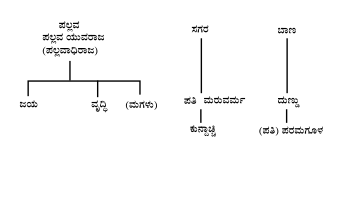
\includegraphics[scale=0.9]{"images/1.jpg"}
\caption{ರಾಮನ್ ಪರಿಣಾಮವನ್ನು ಆವಿಷ್ಕರಿಸಲು ಬಳಸಿದ ಉಪಕರಣಗಳ ಜೊತೆಗೆ, ಸಿ. ವಿ. ರಾಮನ್‍ರವರು}\label{chap1-fig01}
\end{figure}


\begin{figure}
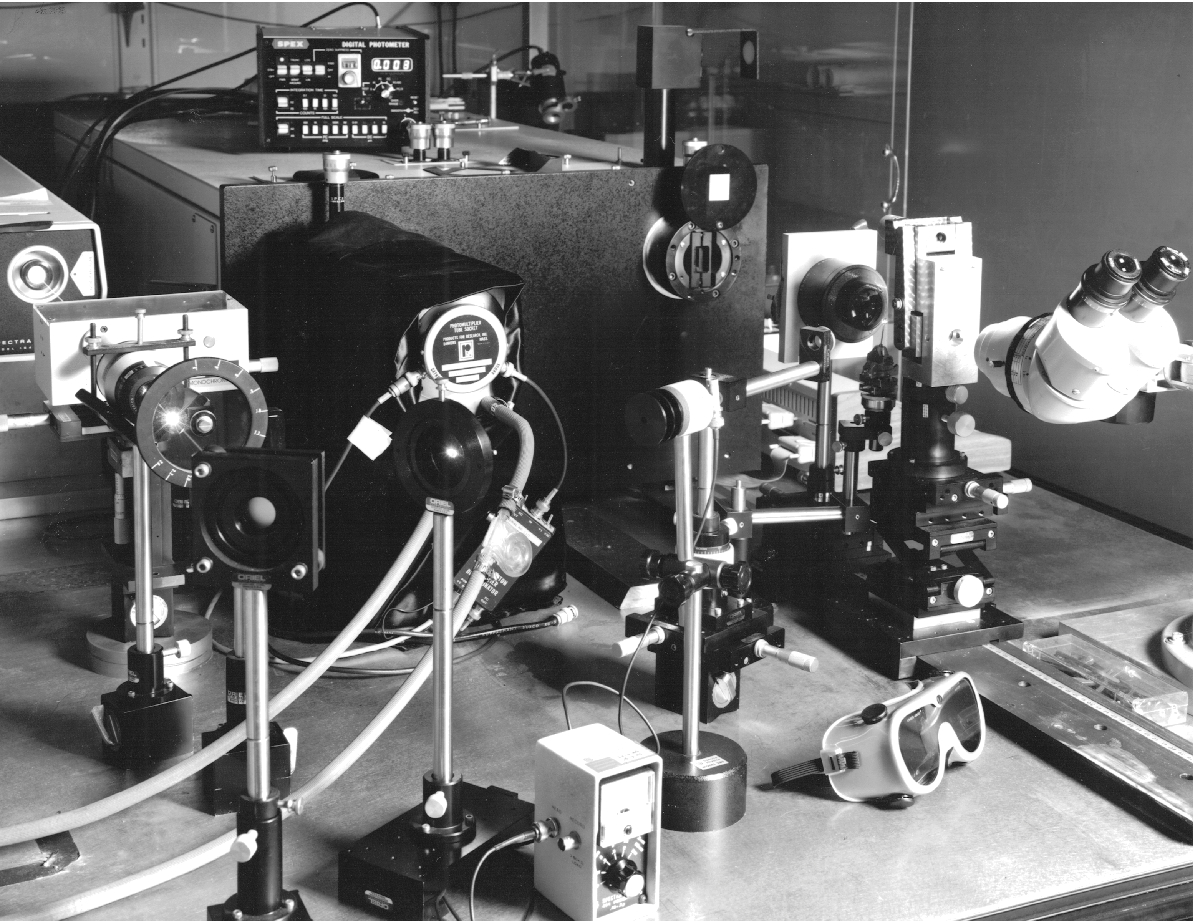
\includegraphics{"images/2.jpg"}
\caption{ಆಧುನಿಕ ಲೇಸರ್ ರಾಮನ್ ರೋಹಿತದರ್ಶಕ}
\end{figure}


\begin{figure}
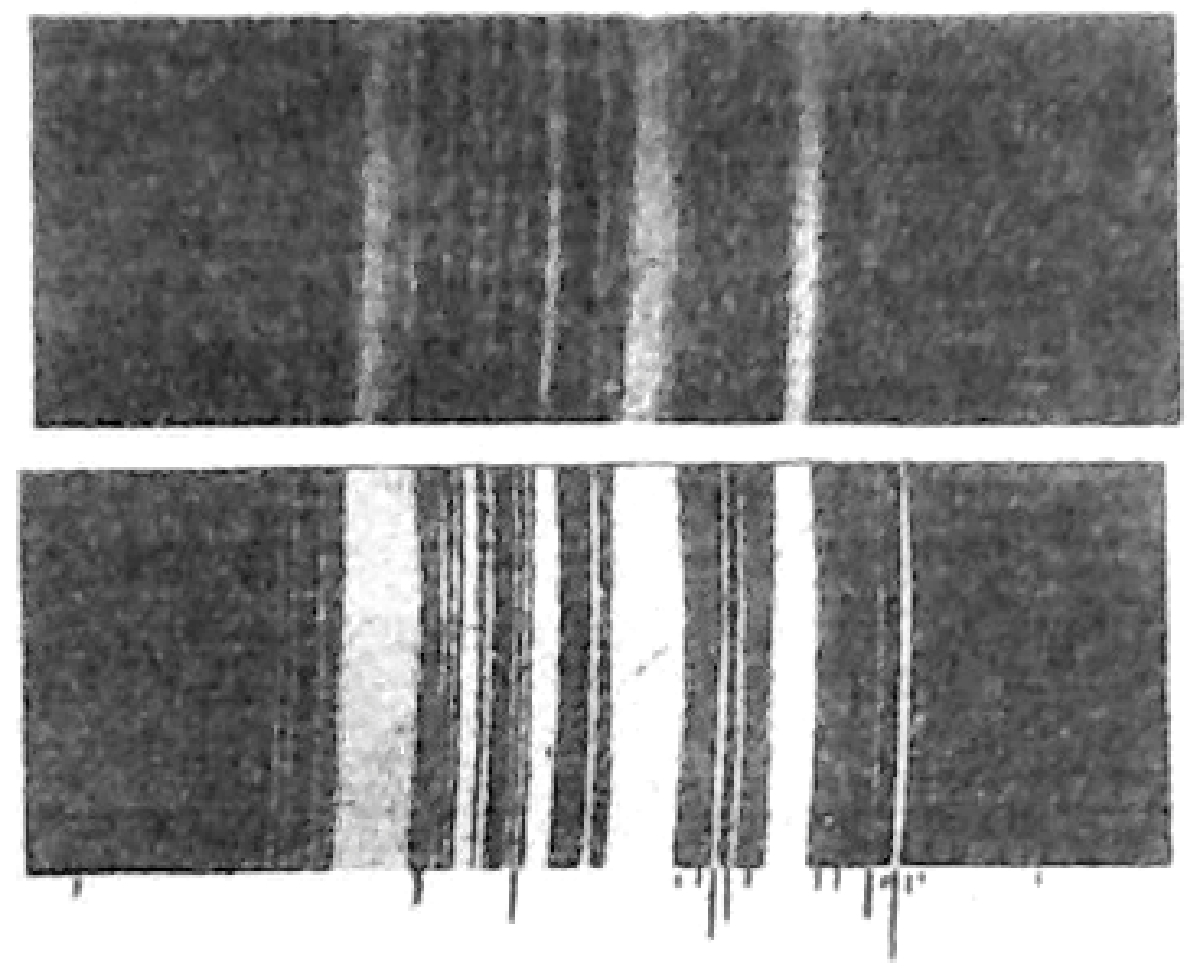
\includegraphics{"images/2a.jpg"}
\caption{ಮರ್ಕ್ಯುರಿ ಆರ್ಕ್ ಬೆಳಕಿನಲ್ಲಿ ಪಡೆದ ಬೆನ್‍ಜೀನ್ ದ್ರವದ ಮೊಟ್ಟ ಮೊದಲ ರಾಮನ್ ರೋಹಿತ \enginline{(Raman spectrum)}}
\end{figure}

ಇದರಲ್ಲಿ ಸ್ಪೋಕ್ಸ್ ಮತ್ತು ಆಂಟಿಸ್ಪೋಕ್ಸ್ ವಿಭಾಗಗಳು ಒಟ್ಟಿಗೆ ಕಂಡವು. \enginline{8} ಮಾರ್ಚ್ ರಂದು ನೇಚರ್ ಪತ್ರಿಕೆಗೆ ರಾಮನ್ ಮತ್ತು ಕೃಷ್ಣನ್ ಅವರುಗಳು ಕಳುಹಿಸಿದ ಸಂಶೋಧನಾ ವಿಚಾರವನ್ನು ಆ ಪತ್ರಿಕೆಯ ರೆಫರೀ ತಿರಸ್ಕರಿಸಿದ್ದರು. ಆದರೆ ಆ ಪತ್ರಿಕೆಯ ಸಂಪಾದಕರಾದ ಸರ್ ರಿಚರ್ಡ್ ಗ್ರಿಗೊರಿ ಅವರು \enginline{21} ಏಪ್ರಿಲ್ ಸಂಚಿಕೆಯಲ್ಲಿ ಇದನ್ನು ಪ್ರಕಟಿಸಿದರು. ಅವರು ತಮ್ಮ ಸ್ವಂತ ಜವಾಬ್ದಾರಿ ಹೊತ್ತುಕೊಂಡು ಈ ಕಾರ್ಯ ಮಾಡಿದ್ದರು.

ರಾಮನ್‍ರವರು ಸಾರ್ವಜನಿಕವಾಗಿ ಈ ಸಂಶೋಧನೆಯ ಪೂರ್ಣ ವಿವರಗಳನ್ನು ಬೆಂಗಳೂರಿನಲ್ಲಿ ಸೌಥ್ ಇಂಡಿಯನ್ ಸೈನ್ಸ್ ಅಸೋಸಿಯೇಷನ್‍ನಲ್ಲಿ \enginline{1928}, \enginline{16} ಮಾರ್ಚ್ ರಲ್ಲಿ ನಡೆದ ಉಪನ್ಯಾಸದಲ್ಲಿ ನೀಡಿದರು. ಈ ಉಪನ್ಯಾಸ ನೀಡಿ ಕಲ್ಕತ್ತಕ್ಕೆ ಮರಳಿದ ಕೂಡಲೇ ಅದೇ ರಾತ್ರಿ ಕೆಲಸ ಮಾಡಿ, ಇದರ \enginline{1000} ಪ್ರತಿಗಳನ್ನು ಪ್ರಿಂಟ್ ಮಾಡಿಸಿದರು. ಅದೇ ದಿನ ಜಗತ್ತಿನ ಎಲ್ಲ ವಿಜ್ಞಾನಿಗಳಿಗೂ ಟಪಾಲು ಮಾಡಿಬಿಟ್ಟರು. ರಾಮನ್ ಮತ್ತು ಕೃಷ್ಣನ್ ಅವರಿಬ್ಬರಿಗೆ ತಮ್ಮ ಆವಿಷ್ಕಾರದ ಗುರುತರ ವಿದ್ಯಮಾನದ ಅರಿವಾಗಿ, ಕಾಂಪ್ಟನ್ ಪರಿಣಾಮದ ಹೋಲಿಕೆಯನ್ನು ಮುಂದೆಂದೂ ತಮ್ಮ ಲೇಖನಗಳಲ್ಲಿ ಎತ್ತಲಿಲ್ಲ. ಕೂಡಲೇ ವಿಜ್ಞಾನ ಪ್ರಪಂಚದಲ್ಲಿ ರಾಮನ್ ಪರಿಣಾಮದ ವಿಷಯವು ಹೊಸ ಸಂಶೋಧನೆಗಳ ವಸ್ತುವಾಯಿತು.

ಮುಂದೆ, ಯೂನಿವರ್ಸಿಟಿ ಆಫ್ ಚಿಕಾಗೋದಲ್ಲಿ ರಾಮನ್‍ರವರ ಅಣ್ಣನ ಮಗನಾದ ಡಾ|| ಚಂದ್ರಶೇಖರ್ ಕೆಲಸ ಮಾಡಿದರು. ರಾಮನ್‍ರವರ ಆವಿಷ್ಕಾರದ ಕಾಲದಲ್ಲಿ ಮದರಾಸಿನ ಪ್ರೆಸಿಡೆನ್ಸಿ ಕಾಲೇಜಿನಲ್ಲಿ ಭೌತಶಾಸ್ತ್ರದ ಆನರ್ಸ್‌ನಲ್ಲಿ ಪ್ರಥಮ ವರ್ಷದ ವಿದ್ಯಾರ್ಥಿಯಾಗಿದ್ದರು. ಅವರು ರಾಮನ್‍ರವರು ಬೆಂಗಳೂರಿಗೆ ಹೋಗುವ ಮುನ್ನ ಮದರಾಸಿನ ತಮ್ಮ ಮನೆಗೆ ಬಂದಿದ್ದುದನ್ನು ಜ್ಞಾಪಿಸಿಕೊಂಡರು. “ಬೆಂಗಳೂರಿಗೆ ಹೊರಡುವ ಮುನ್ನ ರಾಮನ್‍ರವರು ನಮ್ಮ ಮನೆಗೆ ಬಂದಿದ್ದುದು ನನಗೆ ಚೆನ್ನಾಗಿ ಜ್ಞಾಪಕವಿದೆ. ಅಲ್ಲಿ ಅವರು ಆವಿಷ್ಕರಿಸಿದ ರಾಮನ್ ಪರಿಣಾಮವನ್ನು ವಿವರಿಸುವವರಿದ್ದರು. ಸೌಥ್ ಇಂಡಿಯನ್ ಸೈನ್ಸ್ ಅಸೋಸಿಯೇಷನ್ನಿನ ಅಡಿಯಲ್ಲಿ “ಒಂದು ಹೊಸವಿಕಿರಣ” ಎಂಬ ಹೆಸರಿನಲ್ಲಿ ಉಪನ್ಯಾಸ ನೀಡುವವರಿದ್ದರು. ಅವರು ತುಂಬ ಉತ್ಸಾಹಿಗಳಾಗಿದ್ದರು ಮತ್ತು ಸಂತೋಷದಿಂದ ಬೀಗುತ್ತಿದ್ದರು. ಮೊದಲ ರಾಮನ್ ರೋಹಿತವನ್ನು\enginline{(Raman spectrum)} ನಮಗೆಲ್ಲ ತೋರಿಸಿದರು. ಅವರಿಗೆ ಕಾಂಪ್ಟನ್ ಪರಿಣಾಮಕ್ಕೆ (ನೊಬೆಲ್ ಬಹುಮಾನ \enginline{1927}) ಸಂವಾದಿಯಾಗಿ ಸಾಮಾನ್ಯ ಬೆಳಕಿನಲ್ಲಿ ಈ ಪರಿಣಾಮವನ್ನು ಆವಿಷ್ಕರಿಸಿದ ಬಗ್ಗೆ ತುಂಬ ಬಿಗುಮಾನವಿತ್ತು. ರಾಮನ್‍ರವರು ಇದನ್ನು ಒಂದು ವರ್ಷಮೊದಲೇ ಆವಿಷ್ಕರಿಸಿದ್ದರೆ ಏನಾಗುತ್ತಿತ್ತು ಎಂದು ಯಾರೋ ಒಬ್ಬರು ಕೇಳಿದ್ದಕ್ಕೆ ಅವರು ತಕ್ಷಣ “ಆಗ ನೊಬೆಲ್ ಬಹುಮಾನವನ್ನು ಕಾಂಪ್ಟನ್‍ರವರೊಂದಿಗೆ ಹಂಚಿಕೊಳ್ಳ ಬೇಕಾಗುತ್ತಿತ್ತು. ಹಂಚಿಕೊಳ್ಳುವುದು ನನಗಾಗದು. ನನಗೆ ಪೂರ್ತಿ ಬಹುಮಾನವೇ ಬೇಕು” ಎಂದರು. 

ಚಂದ್ರಶೇಖರ್ ರವರು \enginline{1928} ರ ಏಪ್ರಿಲ್, ಮೇ, ಜೂನ್ ತಿಂಗಳುಗಳು ಮತ್ತು \enginline{1929} ರ ಏಪ್ರಿಲ್, ಮೇ ತಿಂಗಳುಗಳನ್ನು ಕಲ್ಕತ್ತದಲ್ಲಿ ಕಳೆದರು. ಅವರು ರಾಮನ್‍ರವರ ಅನೇಕ ಸಹೋದ್ಯೋಗಿಗಳಲ್ಲಿಯೂ ಮುಖ್ಯವಾಗಿ ಕೃಷ್ಣನ್ ಅವರೊಂದಿಗೆ ಸ್ನೇಹ ಸಂಪಾದಿಸಿದರೆಂದು ತಿಳಿಸುತ್ತಾರೆ. “ನನ್ನ ಮೇಲೆ ಅಲ್ಲಿನ ಉತ್ಸಾಹಭರಿತ ವಾತಾವರಣವು ಗಾಢ ಪರಿಣಾಮ ಬೀರಿತು. ಅದು ಇಂದಿಗೂ ಮಾಸಿಲ್ಲ. ಅಲ್ಲಿನ ಎಲ್ಲ ವಿಜ್ಞಾನಿಗಳೂ ತಾವೊಂದು ಅದ್ಭುತ ಆವಿಷ್ಕಾರದಲ್ಲಿ ಭಾಗಿಗಳಾಗಿದ್ದೇವೆಂದು ಆನಂದವಾಗಿದ್ದರು”.

ಇಲ್ಲಿ ಗಮನಿಸಬೇಕಾದ ಅಂಶವೊಂದಿದೆ. ರಾಮನ್‍ರವರು ತಮ್ಮ ಪ್ರಯೋಗ ಕಾರ್ಯದಲ್ಲಿ ತೊಡಗಿದ್ದಾಗಲೇ ಫ್ರಾನ್ಸ್ ಮತ್ತು ರಷ್ಯಾಗಳಲ್ಲಿಯೂ ಇದೇ ದಿಸೆಯಲ್ಲಿ ಪ್ರಯೋಗಗಳು ನಡೆಯುತ್ತಿದ್ದವು. ಕೋಕಾಡ್ ಎಂಬಾತ ಫ್ರೆಂಚ್ ವಿಜ್ಞಾನಿ. ಅವನ ಗಣಿತ ಸಿದ್ಧಾಂತವು ಆಪಾತ ಬೆಳಕಿನ ತರಂಗಾಂತರವು ಅಣುಗಳ ಕಂಪನಗಳಿಂದ ವ್ಯತ್ಯಯಗೊಳ್ಳಬೇಕೆಂದು ಪ್ರತಿಪಾದಿಸಿದ್ದಿತು. ರೋಕಾರ್ಡ್ ಮತ್ತು ಕಬ್ಬಾನೀಸ್ ದ್ವಯರು ಇಂತಹ ವಿದ್ಯಮಾನವನ್ನು ಅನಿಲಗಳಲ್ಲಿ ಹುಡುಕತೊಡಗಿದ್ದರು. ಅನಿಲಗಳಲ್ಲಿ ಬೆಳಕಿನ ಚದರುವಿಕೆಗೆ ಅವಕಾಶ ಕಡಿಮೆ. ಹಾಗಾಗಿ ಅವರು ಈ ಪರಿಣಾಮವನ್ನು ಕಾಣಲಾಗಲಿಲ್ಲ. ಆದರೆ ರಾಮನ್‍ರವರು ದ್ರವಗಳಲ್ಲಿ ಮಾಡಿದ ಪ್ರಯೋಗಗಳಲ್ಲಿ ಬೆಳಕಿನ ಚದರುವಿಕೆಯು ಶಕ್ತವಾಗಿ ಕಂಡಿತು. ರಾಮನ್‍ರವರ ಮೊದಲ ಎರಡು ಸಂಶೋಧನಾ ಪ್ರಬಂಧಗಳನ್ನು ಓದಿದ ಆ ವಿಜ್ಞಾನಿಗಳು ತಮ್ಮ ತಪ್ಪನ್ನು ಅರಿತುಕೊಂಡರು. ತನ್ಮೂಲಕ ರಾಸಾಯನಿಕ ಭೌತಶಾಸ್ತ್ರದ ಮಹತ್ವವನ್ನು ಅರಿತರು.

ಲ್ಯಾಂಡ್ಸ್ ಬರ್ಗ್ ಮತ್ತು ಮಂಡಶ್ಬೆಮ್ ಎಂಬ ರಷ್ಯಾ ದೇಶದ ವಿಜ್ಞಾನಿಗಳು ಸ್ವತಂತ್ರವಾಗಿ ಬೇರೊಂದು ಪ್ರಯೋಗದಲ್ಲಿ ನಿರತರಾಗಿದ್ದರು. ಅವರು ಕ್ವಾರ್ಟ್ಸ್ ಸ್ಫಟಿಕದಲ್ಲಿ ಬೆಳಕಿನ ಚದರುವಿಕೆಯನ್ನು ಅಧ್ಯಯನ ಮಾಡುತ್ತಿದ್ದರು. ಇವರೂ ಸಹ ಮಾರ್ಪಾಡುಗೊಂಡ ರೋಹಿತದಲ್ಲಿ ಭಿನ್ನಗೆರೆ ಇರುವುದನ್ನು ಪ್ರಸ್ತಾಪಿಸಿದ್ದರು. ಆದರೆ ರಾಮನ್‍ರವರು ತಮ್ಮ ಸಂಶೋಧನಾ ಆದ್ಯತೆಯನ್ನು ಬಲವಾಗಿ ಸ್ಥಾಪಿಸಿಬಿಟ್ಟಿದ್ದರು. ಬಹಳ ಮುಂಚಿನಿಂದಲೂ ಅವರ ಧೋರಣೆಯು ಸ್ಪಷ್ಟವಾಗಿದ್ದಿತು. ವೈಜ್ಞಾನಿಕ ಸಂಶೋಧನೆಗಳು ಅತಿ ಶೀಘ್ರವಾಗಿ ಪ್ರಕಟವಾಗಬೇಕು. ಇದನ್ನು ಅವರು ಜೀವನ ಪೂರ್ತಿ ಪಾಲಿಸಿದರು. ಇದೊಂದು ಕಾರಣಕ್ಕಾಗಿಯೇ ಅವರು ಕಲ್ಕತ್ತದಲ್ಲಿ \textit{\general{\enginline{Indian Journal of Physics}}} ನಿಯತಕಾಲಿಕವನ್ನೂ ಬೆಂಗಳೂರಿಗೆ ಬಂದೊಡನೆ \textit{\general{\enginline{Proceedings of Indian Academy of Sciences}}} ಅನ್ನೂ ಶುರು ಮಾಡಿದರು.

ರಾಮನ್‍ರವರು ಬಳಸಿದ ಉಪಕರಣಗಳು: ಸೂರ್ಯನ ಬೆಳಕನ್ನು ವಿಪಥಿಸಲು ಕನ್ನಡಿ, ಕಿರಣಗಳನ್ನು ಕೇಂದ್ರೀಕರಿಸಲು ಮಸೂರ, ಬೆನ್‍ಜೀನ್ ದ್ರವದ ಬಾಟಲು, ಒಂದು ಪಾಕೆಟ್ ರೋಹಿತದರ್ಶಕ, ಇವೆಲ್ಲ ಉಪಕರಣಗಳ ಬೆಲೆ ಕೇವಲ ರೂ.\enginline{500/\general{\enginline{-}}} ಇರಲಿಲ್ಲ. ನಾವು ಹಿಂದೆ ತಿಳಿಸಿದ ವಿಚಾರಗಳಿಂದ ತಿಳಿಯುವ ಅಂಶವೆಂದರೆ ಈ ಆವಿಷ್ಕಾರವು ಆಕಸ್ಮಿಕವಲ್ಲ. ಸತತ ಏಳು ವರ್ಷಗಳ ವ್ಯವಸ್ಥಿತ ಮತ್ತು ಶ್ರಮಭರಿತ ಪ್ರಯೋಗಗಳ ಪರಾಕಾಷ್ಠೆ. ಇದನ್ನು ಕೈಗೊಂಡವರು ರಾಮನ್ ಮತ್ತು ಅವರ ಸಂಗಾತಿ ವಿದ್ಯಾರ್ಥಿಗಳು. ಆಗಿನ ಕಾಲಕ್ಕೆ ನಮ್ಮ ದೇಶದಲ್ಲಿ ವಿಜ್ಞಾನ ಸಂಶೋಧನೆಗೆ ಯಾವ ಉತ್ತೇಜನವೂ ಇರದಿದ್ದಾಗ ಈ ಕಾರ್ಯಸಿದ್ಧಿಯು ಮಹೋನ್ನತವೆ.

ವಿಜ್ಞಾನ ಕ್ಷೇತ್ರ ಪ್ರವೇಶಿಸುವವರಿಗೆ, ರಾಮನ್ ಪರಿಣಾಮದ ಚರಿತ್ರೆಯು ಅನೇಕ ಪಾಠಗಳನ್ನು ಕಲಿಸುತ್ತದೆ. ಒಂದು ಪ್ರಮುಖ ಆವಿಷ್ಕಾರಕ್ಕೆ ಹೆಚ್ಚು ಮೌಲ್ಯದ ಉಪಕರಣಗಳು ಅವಶ್ಯವೆನಿಸುವುದಿಲ್ಲ, ಬದಲಿಗೆ ವಿಜ್ಞಾನಿಗಳ ಸಾಮರ್ಥ್ಯ, ನಿರಂತರ ದುಡಿಮೆ ಮತ್ತು ಏಕಾಗ್ರತೆಗಳು ಮುಖ್ಯ. ಯಾವುದೇ ಆವಿಷ್ಕಾರವಾಗಲಿ ನೇರವಾಗಿ, ಸ್ಪಷ್ಟವಾಗಿ ತೋರುವುದು ಅಪರೂಪ. ಪ್ರಕೃತಿಯು ತನ್ನ ಗೌಪ್ಯಗಳನ್ನು ಸ್ವಲ್ಪ ಸ್ವಲ್ಪವಾಗಿ ಹೊರಗೆಡುತ್ತದೆ. ಹಿರಿಯ ಆವಿಷ್ಕಾರಗಳು ನಮಗೆ ಸರಳವಾಗಿ ಕಾಣುವುದು ಬೇರೊಬ್ಬರು ವಿವರಿಸಿದ ಮೇಲೆಯೇ.


\heading{ಸಾಮಿರ್‌ಫೀಲ್ಡ್‌ರವರ ಕಲ್ಕತ್ತ ಭೇಟಿ}

\enginline{1928}ರಲ್ಲಿ ಸಾಮಿರ್‍ಫೀಲ್ಡ್ ನಂತಹ ಉನ್ನತ ದರ್ಜೆಯ ವಿಜ್ಞಾನಿಗಳು ಕಲ್ಕತ್ತದ ರಾಮನ್ ಲ್ಯಾಬೊರೇಟರಿಗೆ ಬಂದದ್ದು ಅತಿ ದೊಡ್ಡ ಮಾತೇ ಸರಿ. ಅವರು ಅಲ್ಲಿಗೆ ಬಂದು ರಾಮನ್‍ರವರ ಆವಿಷ್ಕಾರದ ಪ್ರಾತ್ಯಕ್ಷಿಕೆ ಪಡೆದರು. ಆಗ ವಿದೇಶಗಳಲ್ಲಿ ತೀವ್ರತೆಯಿಲ್ಲದ, ಇಂತಹ ಕ್ಷೀಣ ವಿಕಿರಣವನ್ನು ರಾಮನ್‍ರವರು ವೀಕ್ಷಿಸಲು ಸಾಧ್ಯವೇ ಎಂದು ಸಂಶಯ ಪಡುವ ಜನರಿದ್ದರು. ಸಾಮಿರ್‍ಫೀಲ್ಡ್ ಅವರು \enginline{1928} ಅಕ್ಟೋಬರ್‍ನಲ್ಲಿ ಬಂದರು. ರಾಮನ್‍ರವರು ತಮ್ಮ ಆವಿಷ್ಕಾರವನ್ನು ತೋರಿಸಿದರು. ಸಾಮಿರ್‌ಫೀಲ್ಡ್‌ರವರಿಗೆ, ವಿಜ್ಞಾನ ಸಂಶೋಧನೆಯಲ್ಲಿನ, ರಾಮನ್‍ರವರ ತೀವ್ರ ಸಮರ್ಪಣಾ ಭಾವವು ಇಷ್ಟವಾಯಿತು. ಅವರಿಗೆ ಪ್ರಯೋಗಗಳ ಪ್ರಾತ್ಯಕ್ಷಿಕೆಗಳೂ ಮೆಚ್ಚುಗೆಯಾದವು.

\begin{figure}
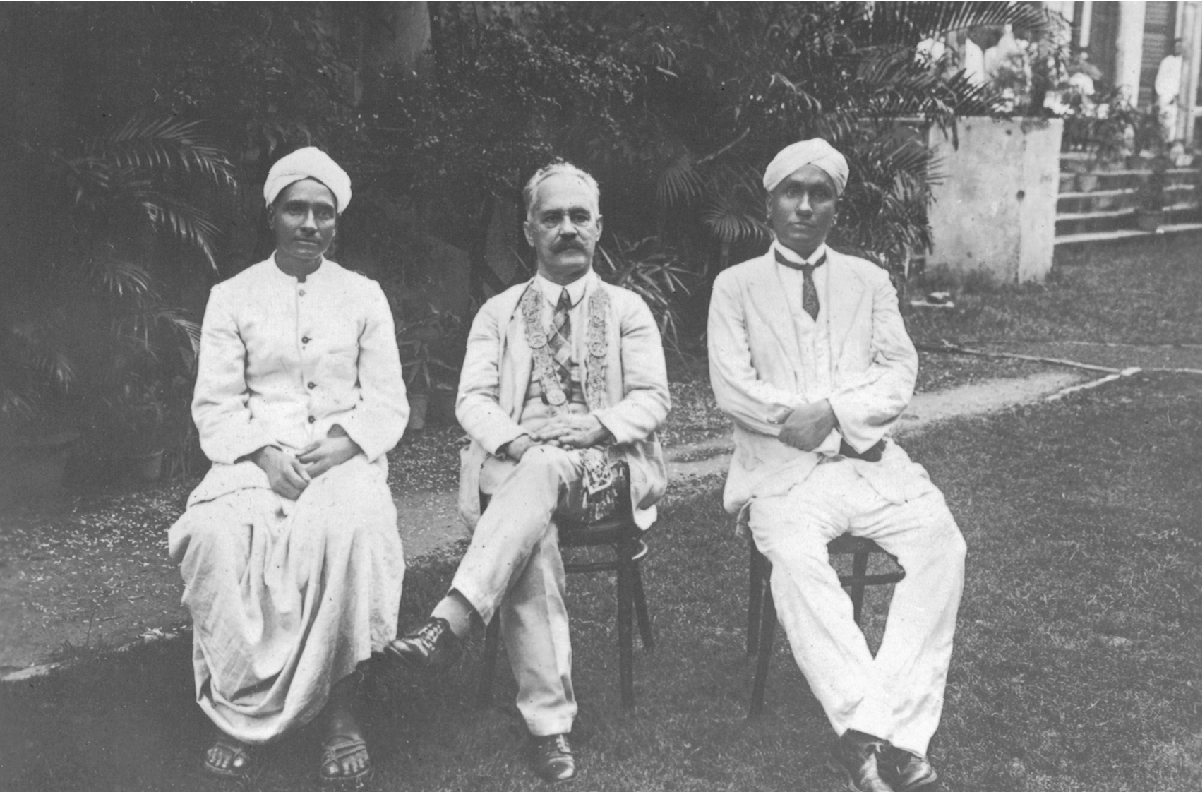
\includegraphics{"images/3.jpg"}
\caption{\enginline{1928}ರಲ್ಲಿ ಕಲ್ಕತ್ತದಲ್ಲಿ ತೆಗೆದ ಚಿತ್ರ. ಆರ್ನಾಲ್ಡ್ ಸಾಮಿರ್‌ಫೀಲ್ಡ್‌ರವರು ಸಿ. ವಿ. ರಾಮನ್ (ಬಲ), ಕೆ. ಎಸ್. ಕೃಷನ್ (ಎಡ)ರವರೊಡನೆ (ಫೋಟೋ ಕೃಪೆ: ಲುಡ್‍ವಗ್\enginline{-}ಮ್ಯಾಕ್ಸಿಮಿಲಿಯನ್ ಯುನಿವರ್ಸಿಟಿಯ ಡಾ. ಜಿ. ತೋರ್ಕರವರು ನೀಡಿದ್ದು. ಡಾಯಿಷ್ ಮ್ಯೂಸಿಯಮ್, ಮ್ಯೂನಿಕ್‍ನಲ್ಲಿದೆ)}
\end{figure}

ಆರ್ನಾಲ್ಡ್ ಸಾಮಿರ್‍ಫೀಲ್ಡ್ ಅವರಿಗೆ ಅಮೆರಿಕಾದಲ್ಲಿ ಒಂದೆರಡು ತಿಂಗಳು ಅತಿಥಿ ಪ್ರೊಫೆಸರ್ ಆಗಿರಲು ಆಹ್ವಾನ ಬಂದಾಗ (\enginline{1929}), ಅವರು “ಸಾಮಾನ್ಯವಾದ ದಾರಿ ಬಿಟ್ಟು, ಅಸಾಮಾನ್ಯವಾದ ಪೂರ್ವದೇಶಗಳ ದಾರಿಯ ಮೂಲಕ” ಅಮೆರಿಕಾಗೆ ಹೋಗುವ ತೀರ್ಮಾನ ಕೈಗೊಂಡಿದ್ದರು. ಅವರಿಗೆ ಭಾರತದ ಆಕರ್ಷಣೆ ತೀವ್ರವಾಗಿತ್ತು. ಅವರಿಗೆ ಇಲ್ಲಿನ ಅದ್ಭುತಗಳೂ, ಪ್ರಾಚೀನ ನಾಗರಿಕತೆಯೂ ಮತ್ತು ಉನ್ನತ ಧಾರ್ಮಿಕ ಮತ್ತು ತತ್ತ್ವಶಾಸ್ತ್ರ ಪದ್ಧತಿಗಳೂ ಆಸಕ್ತಿಯ ವಿಷಯಗಳಾಗಿದ್ದವು. ಅಲ್ಲದೆ ಇಲ್ಲಿನ ವೈಜ್ಞಾನಿಕ ಕಾರ್ಯದ ಬಗ್ಗೆ ಅತ್ಯಾಧುನಿಕ ಅಧ್ಯಯನಗಳ ಬಗ್ಗೆ ಅದರಲ್ಲೂ ಜಗತ್ತಿನ ಶ್ರೇಷ್ಠ ಮಟ್ಟದ ವಿಜ್ಞಾನಿಗಳಾಗಿ ಬೆಳೆಯುತ್ತಿದ್ದ ರಾಮನ್‍ರವರ ಬಗ್ಗೆ ಒಳ್ಳೆಯ ಅಭಿಪ್ರಾಯವಿತ್ತು. ಅದಕ್ಕಾಗಿಯೇ ಸಾಮಿರ್‍ಫೀಲ್ಡ್ ಅವರು ಭಾರತದ ಮೂಲಕ ಪಯಣಿಸಿದರು. ಇದು ರಾಮನ್‍ರವರು ತಮ್ಮ ಆವಿಷ್ಕಾರವನ್ನು ಶೋಧಿಸುವ ಮೊದಲೇ ತೆಗೆದುಕೊಂಡ ತೀರ್ಮಾನ.

\enginline{1928}, ಫೆಬ್ರವರಿ \enginline{11}ರಲ್ಲಿ ರಾಮನ್‍ರವರು ಸಾಮಿರ್‌ಫೀಲ್ಡ್‌ರವರಿಗೆ ತಂತಿ ಕಳುಹಿಸಿದ್ದರು\enginline{-} “ಕಲ್ಕತ್ತ ವಿಶ್ವವಿದ್ಯಾಲಯವು ಆಹ್ವಾನಿಸುತ್ತಿದೆ. ಸಂಭಾವನೆ ಒಂದು ಸಾವಿರ ರೂಪಾಯಿಗಳು, ಭಾರತಕ್ಕೆ ಬರುವ ದಿನವನ್ನು ತಂತಿಯ ಮೂಲಕ ತಿಳಿಸಿ”.

ಸಾಮಿರ್‍ಫೀಲ್ಡ್ ಅವರಿಗೆ ಭಾರತದಿಂದ ಅನೇಕ ಆಹ್ವಾನಗಳು ಬಂದಿದ್ದವು. ಆಧುನಿಕ ಭೌತಶಾಸ್ತ್ರದ ಬಗ್ಗೆ ಅನೇಕ ಭಾರತೀಯ ಯೂನಿವರ್ಸಿಟಿಗಳಲ್ಲಿ ಉಪನ್ಯಾಸ ನೀಡುವುದೂ ಅಲ್ಲದೆ ಮೇಘನಾದ ಸಹಾ ಅವರು ತಯಾರಿಸಿದ ಪ್ರಯಾಣ ಮಾರ್ಗ ಪಟ್ಟಿಯಲ್ಲಿದ್ದ ವಿವಿಧ ಪ್ರೇಕ್ಷಣೀಯ ಸ್ಥಳಗಳಿಗೆ ಭೇಟಿ ಮುಖ್ಯವಾದುವು. ಆದರೆ ಅವರು ಭಾರತಕ್ಕೆ ಬರುತ್ತಿದ್ದಂತೆಯೇ ಖಾಯಿಲೆ ಬಿದ್ದರು. ಎರಡು ವಾರಗಳವರೆಗೆ ಬೆಂಗಳೂರಿನಲ್ಲಿ ಚಿಕಿತ್ಸೆ ಪಡೆದರು. ಹಾಗಾಗಿ ಅವರು ಭಾರತಕ್ಕೆ ಬರಲು ಮುಖ್ಯ ಕಾರಣವಾದ ಕಲ್ಕತ್ತೆಗೆ \enginline{1928}, ಅಕ್ಟೋಬರ್ \enginline{4}ರಂದು ಬರಲು ಸಾಧ್ಯವಾಯಿತು. ಅವರ ಡೈರಿಯಲ್ಲಿ ನಮೂದಿಸಿದಂತೆ ಅವರು ಕಲ್ಕತ್ತದಲ್ಲಿ ಸಮಯ ಕಳೆದದ್ದು ಹೀಗೆ:

ಅಕ್ಟೋಬರ್ \enginline{4}: ಹೌರಾ ಸ್ಟೇಶನ್ ನಲ್ಲಿ ಅಭೂತಪೂರ್ವ ಸ್ವಾಗತ. ರಾಮನ್, ಬೋಸ್, ಕೃಷ್ಣನ್, ಸೇನ್, ಘೋಷ್ ಮಿತ್ರ..... ಅಲ್ಲದೆ ನನ್ನ ವಾಸ ನಿಗದಿಯಾಗಿದ್ದ ಜರ್ಮನ್ ವೈಸ್ ಕೌನ್ ಸೆಲ್ ಎಬ್ರೆಲ್,....... ಇವರ ಮನೆಯಲ್ಲಿ \enginline{3} ಸುಂದರ ರೂಮಗಳು, ಬಾತ್ ರೂಂ ಸಹಿತ ನನಗಾಗಿ...... ದಾಸವಾಳ ಹೂಗಳು ಮೊದಲ ಮಹಡಿಯವರೆಗೆ ಎದ್ದು ನಿಂತಿದ್ದವು....... ಬೋಸ್ ನನ್ನನ್ನು ರಾಮನ್‍ರವರ ಸಂಸ್ಥೆಗೆ ಕರೆದುಕೊಂಡು ಹೋದರು...... ಅವರು ವಿವರ್ತನದ ಬಗ್ಗೆ ಪ್ರಬಂಧ ತೋರಿಸಿದರು.

ಅಕ್ಟೋಬರ್ \enginline{6}: ಬೆಳಿಗ್ಗೆ \enginline{8} ಗಂಟೆಗೆ ಕೆಪ್ಲರ್‍ನ ಸಮಸ್ಯೆಗಳ ಬಗ್ಗೆ ಮೊದಲ ಉಪನ್ಯಾಸ, \enginline{10} ಗಂಟೆಯವರೆಗೆ ಚರ್ಚೆ..... ಬಳಿಕ ರಾಮನ್ ಪರಿಣಾಮವನ್ನು ಕಣ್ಣಿನಲ್ಲಿ ನೋಡಿದ್ದು; ನೀಲಿ ಫಿಲ್ಟರ್ ಪೂರಕ ಸ್ಕ್ರೀನ್; ಆಪಾತ ಬೆಳಕಿನ ಮುಂದೆ. ಅನಂತರ ಚದರಿದ ಬೆಳಕಿನ ಮುಂದೆ ಇಟ್ಟಿದ್ದು...... ವ್ಯತ್ಯಾಸ.

ಅಕ್ಟೋಬರ್ \enginline{7}: ಭಾನುವಾರ....... ರಾಮನ್ ಅವರಿಂದ ಅದ್ಭುತ ಉಪನ್ಯಾಸ (ಹಾಗೂ ಅಣುಗಳ ಭ್ರಮಣವನ್ನು ವಿವರಿಸಲಾಗಿಲ್ಲ, ಮಾರ್ಪಾಡಾದ ವಿಕರಣ.....) 

ಅಕ್ಟೋಬರ್ \enginline{8–13: 8–10} ರವರೆಗೆ ಉಪನ್ಯಾಸಗಳು ಆಕರ್ಷಕ ಚರ್ಚೆಗಳು...... 

“ನಾನು ಈ ಸಂಸ್ಥೆಯಲ್ಲಿ ಮಂಜುಗಡ್ಡೆಯ ಮೇಲೆ ನೀಲಿ\enginline{-}ಹಸಿರು ಬೆಳಕಿನ ಚದರುವಿಕೆಯನ್ನು ನೋಡಿದೆ, ಅದು ಮಾರ್ಪಾಡುಗೊಂಡ ಚದರು ಬೆಳಕೇ. ಸಂಸ್ಥೆಯಲ್ಲಿ ಎಲ್ಲವೂ ಬಹಳ ಚೆನ್ನಾಗಿದೆ ಬಾತ್ ರೂಂಗಳು ಮಾತ್ರ ಭಯಂಕರವಾಗಿವೆ.”...........

ಭಾರತದಲ್ಲಿ ಸಾಮಿರ್‍ಫೀಲ್ಡ್‌ರವರ ಆಸಕ್ತಿಗಳು ಭೌತಶಾಸ್ತ್ರಕ್ಕೆ ಮಾತ್ರ ಸೀಮಿತವಾಗಿರಲಿಲ್ಲ. ಅವರಿಗೆ ಇಲ್ಲಿ ಜನಜೀವನ ಮತ್ತು ಕಲೆಗಳ ಬಗ್ಗೆ ತೀವ್ರ ಆಸಕ್ತಿಯಿತ್ತು. ಉತ್ತರ ಭಾರತದಲ್ಲಿನ ಕೆಲವು ಪ್ರೇಕ್ಷಣೀಯ ಸ್ಥಳಗಳನ್ನು ನೋಡಲು \enginline{14} ಅಕ್ಟೋಬರ್ ರಂದು ಕಲ್ಕತ್ತದಿಂದ ಹೊರಟರು. ಅವರು ನೋಡಬೇಕಾದ ಸ್ಥಳಗಳಲ್ಲಿ ಬೆನಾರಸ್ ಮತ್ತು ಆಗ್ರಾಗಳಿದ್ದವು. ದೆಹಲಿಯನ್ನು ನೋಡುವುದಕ್ಕಿಂತಲೂ ಶಾಂತಿನಿಕೇತನಕ್ಕೆ ಹೋಗಲು ಆಶಿಸಿದ್ದರು. ಅಂದಿಗೆ ಸಾಹಿತ್ಯಕ್ಕಾಗಿ ನೊಬೆಲ್ ಬಹುಮಾನ ಪಡೆದಿದ್ದ ಟಾಗೂರರು, ಅವರನ್ನು ಆಹ್ವಾನಿಸಿದ್ದರು. ಈ ಆಹ್ವಾನವನ್ನು ಬಹಳ ಮೆಚ್ಚುಗೆಯಿಂದ ಸಾಮಿರ್‍ಫೀಲ್ಡ್ ಸ್ವೀಕರಿಸಿದ್ದರು. ಜರ್ಮನ್ ಕವಿ ಗೊಯ್ತೆಗೆ ಸರಿಸಮಾನವಾಗಿ ಟಾಗೊರ್‍ರನ್ನು ಸಮೀಕರಿಸುತ್ತಿದ್ದ ಅವರು, ಶಾಂತಿನಿಕೇತನದಲ್ಲಿ “ಭಾರತದಲ್ಲಿ ಶರತ್ ಕಾಲದ ಒಂದು ಶಾಂತಿಯ ದಿನವಾಗಿ” ಅನುಭವಿಸಿದರು. ಅಕ್ಟೋಬರ್ \enginline{26} ರಂದು ಸಾಮಿರ್‍ಫೀಲ್ಡ್ ಭಾರತವನ್ನು ಬಿಟ್ಟರು. ಎರಡು ಕಾರುಗಳು ಬಂದರ್ ವರೆಗೆ ಬಂದವು..... ಕೃಷ್ಣನ್ ಅವರಿಂದ ಹೂಮಾಲೆಯ ಧಾರಣೆಯಾಯಿತು, ಎಕ್ಸರೇ ಮಾನವನಿಂದ ಹೂಗುಚ್ಛ.......” ಹೊರಡುವ ಮುನ್ನ ರಾಮನ್ ಅವರೊಂದಿಗಿನ ಸಂಭಾಷಣೆಯನ್ನು ದಾಖಲಿಸಿದ್ದಾರೆ. ಇದರಲ್ಲಿ ಅವರ ಸ್ಮೃತಿಗಳೂ, ಪ್ರವಾಸದ ಅನುಭವಗಳೂ ಇವೆ. ಇದರಲ್ಲಿ ಭಾರತದ ಆರ್ಥಿಕತೆ ಮತ್ತು ರಾಜಕೀಯ ಸಂದರ್ಭಗಳನ್ನು ಕುರಿತು ಕಟು ವಿಮರ್ಶೆಗಳಿವೆ. ದೇಶದ ಮತ್ತು ಬ್ರಿಟನ್ನಿನ ನಡುವೆಯ ಸಂಕಷ್ಟಕರ ಬಾಂಧವ್ಯ ಕುರಿತೂ ಮಾತುಗಳಿವೆ. “ಗರಿಷ್ಠ ಸಂಸ್ಕೃತಿಯ ದುಃಖಭರಿತ ರಾಷ್ಟ್ರಕ್ಕೆ ನನ್ನ ಹೃದಯ ತುಂಬಿ ಬಂದಿದೆ. ಇಲ್ಲಿ ನನ್ನನ್ನು ಗೌರವಿಸಿ, ಸ್ನೇಹ ತೋರಿದವರಿಗೆ ನಾನು ಆಭಾರಿಯಾಗಿದ್ದೇನೆ ಎಂದು ದಾಖಲಿಸಿ ಭಾರತದಿಂದ ಹೊರಟರು. ಅವರಿಗುಂಟಾದ ಕೃತಜ್ಞತೆಯ ಭಾರದಲ್ಲಿ ರಾಮನ್‍ರವರನ್ನು ನೊಬೆಲ್ ಬಹುಮಾನಕ್ಕೆ ಶಿಫಾರಸ್ ಮಾಡಿದರು. ಈ ವಿಷಯವು ರಾಮನ್ ಅವರಿಗೆ ತಿಳಿದಾಗ ಅವರು ಮನಃತುಂಬಿ ಸಾಮಿರ್‍ಫೀಲ್ಡ್ ಅವರನ್ನು ಅಭಿನಂದಿಸಿದರು\enginline{-} “ನಿಮ್ಮ ಈ ಕರುಣಾಭರಿತ ಕಾರ್ಯಕ್ಕೆ ನಾನು ಹೇಗೆ ಕೃತಜ್ಞತೆ ತಿಳಿಸಬೇಕೆಂದು ಅರಿವಾಗುತ್ತಿಲ್ಲ. ನನ್ನ ಹೊಸ ಪರಿಣಾಮದ ಬಗ್ಗೆ ಸಾಕಷ್ಟು ಶೀಘ್ರವಾಗಿ ಅಧ್ಯಯನಗಳು ನಡೆಯುತ್ತಿವೆ. ಡಿಸೆಂಬರ್‍ನಲ್ಲಿ ನಿರ್ಧಾರವಾಗುವ ನೊಬೆಲ್ ಕಮಿಟಿಯಲ್ಲಿ ನನ್ನ ಹೆಸರಿಗೆ ಬೆಂಬಲ ಸಿಗಬಹುದೇನೋ”.

ನೊಬೆಲ್ ಬಹುಮಾನ ಪಡೆದ ನಂತರ ರಾಮನ್‍ರವರು, ಸಾಮಿರ್‍ಫೀಲ್ಡ್ ಅವರನ್ನು ಮ್ಯೂನಿಕ್ ನಗರದಲ್ಲಿ ಭೇಟಿಯಾದರು. ಇವರನ್ನು ಅತ್ಯಂತ ಆದರ ಆನಂದಗಳಿಂದ ಅವರು ಬರಮಾಡಿಕೊಂಡರು. “ನಾವು ಈ ಅತಿಥಿಯನ್ನು ಶ್ರೇಷ್ಠ ವಿಜ್ಞಾನಿ ಸಂಶೋಧಕನೆಂದು, ಮಾತ್ರ ಬರಮಾಡಿಕೊಳ್ಳುತ್ತಿಲ್ಲ ಬದಲಿಗೆ ಅತಿ ಪುರಾತನ ಹಾಗೂ ಇಂದಿಗೆ ಪುನರುಜ್ಜೀವನ ಕಾಣುತ್ತಿರುವ ಪೂರ್ವದೇಶದ ಸಂಸ್ಕೃತಿಯ ರಾಯಭಾರಿಯಾಗಿಯೂ ಕಾಣುತ್ತೇವೆ. ಈ ಸಂಸ್ಕೃತಿಯು ಪಶ್ಚಿಮದ ಸಂಸ್ಕೃತಿಯೊಂದಿಗೆ ಮನಸ್ಫೂರ್ತಿ ಸಹಕಾರ ನೀಡಿ ಒಂದೇ ಗುರಿಯತ್ತ ಮುನ್ನುಗ್ಗುತ್ತಿದೆ”.

\enginline{1929}ರಲ್ಲಿ ರಾಮನ್‍ರವರ ಹೆಸರನ್ನು ನೊಬೆಲ್ ಬಹುಮಾನಕ್ಕೆ ಶಿಫಾರಸು ಮಾಡಿದವರು ನೀಲ್ಸ್ ಭೊರ್ ಮತ್ತು ಸಿ.ಫೆಬ್ರೇ. \enginline{1930}ರಲ್ಲಿ ಇ.ಬ್ಲಾಚ್, ನೀಲ್ಸ್ ಭೋರ್, ಡಿಬ್ರಾಗ್ಲಿ (ತಂದೆ, ಮಗ), ಓ.ಖ್ವೊಲ್ ಸನ್, ಜಿ.ಪೆರ್ರಿನ್, ಆರ್.ಫೈಪರ್, ಇ.ರುದರ್ ಫರ್ಡ್, ಜಿ.ಸ್ಟಾಕ್ ಮತ್ತು ಸಿ. ಟಿ. ಆರ್.ವಿಲ್ ಸನ್. ಇವರಲ್ಲಿ ಸಾಮಿರ್‍ಫೀಲ್ಡ್ ಅವರ ಹೆಸರಿಲ್ಲವೇ ಇಲ್ಲ. ಬಹುಶಃ ಇವರು ನೊಬೆಲ್ ಕಮಿಟಿಗೆ ಬರೆದ ಪತ್ರ ಅಧಿಕೃತವಾಗಿ ದಾಖಲಾಗದೇ ಇದ್ದಿರಬಹುದು. ರಾಮನ್ ಅವರಿಗೆ \enginline{1930}ರಲ್ಲಿ ನೊಬೆಲ್ ಬಹುಮಾನ ಸಿಕ್ಕಿತು. ಇದಕ್ಕೆ ಸಾರ್ವತ್ರಿಕವಾಗಿ ಸ್ವಾಗತ ಸಿಕ್ಕಿತು. ಆಗ ರಾಮನ್ ಅವರಿಗೆ \enginline{42} ರ ವಯೋಮಾನ. ಅವರು ಮತ್ತು ಲೇಡಿ ರಾಮನ್‍ರವರು ಸ್ಟಾಕ್‍ಹೋಂಗೆ ನೊಬೆಲ್ ಬಹುಮಾನ ಸ್ವೀಕರಿಸಲು \enginline{1930}ರ ಡಿಸೆಂಬರ್ \enginline{10} ರಂದು ಹೊರಟರು.

ನೊಬೆಲ್ ಸಮಿತಿಯ ಸಭೆಗಳು ಅತ್ಯಂತ ಗೌಪ್ಯವಾಗಿ ನಡೆಯುತ್ತವೆ. ಸಾಮಾನ್ಯವಾಗಿ ನವೆಂಬರ್‍ನಲ್ಲಿ ಬಹುಮಾನ ಘೋಷಣೆ ಮಾಡುತ್ತಾರೆ. ಡಿಸೆಂಬರ್ ಮಧ್ಯ ಭಾಗದಲ್ಲಿ ಸಮಾರಂಭ ನಡೆಯುವ ಕೇವಲ ಒಂದು ತಿಂಗಳ ಮುಂಚೆ, ರಾಮನ್ ಅವರಿಗೆ ಬಹುಮಾನದ ತಂತಿ ಬಂದ ಬಳಿಕ ಅವರು ಹೊರಡಲು ತಯಾರಿ ನಡೆಸಿದ್ದರೆ, ಆಗಿನ ಕಾಲದ ಉಗಿ ಹಡಗುಗಳ ಪಯಣದಲ್ಲಿ ಸಮಾರಂಭದ ವೇಳೆಗೆ ಸ್ಟಾಕ್‍ಹೊಂ ತಲುಪುವುದು ಅಸಾಧ್ಯವಾಗಿತ್ತು. ಈಗ ಚರಿತ್ರೆಯ ಸತ್ಯ ಹೊರಬಿದ್ದಿದೆ. ರಾಮನ್‍ರವರು ತಮಗೂ ತಮ್ಮ ಪತ್ನಿಗೂ ಜುಲೈ ತಿಂಗಳಿನಲ್ಲೇ ಎರಡು ಟಿಕೆಟ್ ಬುಕ್ ಮಾಡಿಸಿಕೊಂಡಿದ್ದರು. ಬಹುಮಾನದ ಘೋಷಣೆಗೆ ನಾಲ್ಕು ತಿಂಗಳ ಮೊದಲು, ಡಿಸೆಂಬರ್‍ನ ಮೊದಲವಾರದಲ್ಲೇ ಅಲ್ಲಿ ಹಾಜರಾಗಿದ್ದರು.


\heading{ಸ್ಟಾಕ್‍ಹೋಂ ಮತ್ತು ನೊಬೆಲ್ ಸಮಾರಂಭ}

\enginline{1931}ರಲ್ಲಿ ಕಲ್ಕತ್ತ ಮುನಿಸಿಪಲ್ ಕಾರ್ಪೋರೇಷನ್ ನವರು \textit{\general{\enginline{Address to Prof. Raman}}} (ರಾಮನ್ ಅವರಿಗೊಂದು ಬಿನ್ನವತ್ತಳೆ) ಎಂಬ ಶೀರ್ಷಿಕೆಯಲ್ಲಿ ಕಲ್ಕತ್ತ ಮುನಿಸಿಪಲ್ ಗೆಜೆಟ್ ಹೊರಡಿಸಿದರು. ಇದು \enginline{Raman Number} (ರಾಮನ್ ಪುರವಣಿ) ಎಂದೇ ಹೆಸರಾಯಿತು. ಇದರಲ್ಲಿ ಸ್ಟಾಕ್‍ಹೋಂನಲ್ಲಿ ನಡೆದ ನೊಬೆಲ್ ಸಮಾರಂಭವನ್ನು ಕಣ್ಣಿಗೆ ಕಟ್ಟುವಂತೆ ವಿವರಿಸಿದ್ದಾರೆ. ‘ಸ್ಟಾಕ್‍ಹೋಂ ನಲ್ಲಿ ಒಂದು ವಾರ’ ಎಂಬ ಪ್ರಬಂಧವನ್ನು ಲೇಡಿ ರಾಮನ್ ಬರೆದಿದ್ದಾರೆ. ಅದರಲ್ಲಿ\enginline{-} “ಸ್ವೀಡನ್‍ನಲ್ಲಿ ನಾವು ಕಳೆದ ಒಂದು ವಾರ ಹಬ್ಬದ ವಾತಾವರಣ, ಭಾರತದಲ್ಲಿದ್ದಂತೆ ಹೂಮಾಲೆಗಳೇನಾದರೂ ಸ್ವೀಡನ್‍ನ ಸಂಪ್ರದಾಯವಾಗಿದ್ದರೆ, ಅದು ಬೆಟ್ಟದಷ್ಟಾಗುತ್ತಿತ್ತು. ಆದರೆ ಅಲ್ಲಿ ಫೋಟೋ ಕ್ಲಿಕ್ಕಿಸುವುದೇ ದೊಡ್ಡ ಸಂಭ್ರಮ. ಬಾಲ್ಟಿಕ್ ಸಮುದ್ರದಲ್ಲಿ ಸ್ವೀಡನ್‍ಗೆ ಪಯಣಿಸುವ ದೋಣಿಯಲ್ಲಿಯೂ ಪತ್ರಿಕಾ ವರದಿಗಾರರಿದ್ದರು. ಇತರ ದೇಶಗಳಲ್ಲಿ ನೊಬೆಲ್ ಬಹುಮಾನವೇತ್ತರನ್ನು ಹೇಗೆ ನೋಡುವರೆಂದು ನನಗೆ ಗೊತ್ತಿಲ್ಲ. ಆದರೆ ಸ್ವೀಡನ್‍ನ ಕಣ್ಣಿಗೆ ಅವರು ವಿಶೇಷವಾಗಿ ಕಾಣುತ್ತಾರೆ. ಭಾರತದಲ್ಲಿ ಅತಿಥಿಗಳ ಉಪಚಾರವನ್ನು ಧಾರ್ಮಿಕವಾಗಿ ನೋಡುತ್ತಾರೆ. ಆದರೆ ಅತಿಥ್ಯವೆಂದರೆ ಏನು ಎಂಬುದನ್ನು ಸ್ವೀಡನ್‍ನಲ್ಲಿ ನೋಡಿದೆ.

ಸ್ಟಾಕ್‍ಹೋಂನಲ್ಲಿ ನಮ್ಮ ವಾಸ್ತವ್ಯವು ವಾರದ ಮಟ್ಟಿಗೆ ಅಂದರೆ ಡಿಸೆಂಬರ್ \enginline{9} ರಿಂದ \enginline{16} ವರೆಗೆ (\enginline{1930}) ಮುಂದುವರಿಯಿತು. ಸ್ವೀಡನ್‍ನ ರಾಜಧಾನಿಯಾದ ಸ್ಟಾಕ್‍ಹೋಂಗೆ ನಾವು ಟ್ರೈನ್‍ನಲ್ಲಿ ಬಂದಿಳಿದೆವು. ಅತಿಥಿಗಳನ್ನು ಬರಮಾಡಿಕೊಳ್ಳಲು ಪ್ಲಾಟ್‍ಫಾರ್ಮ್‌ನಲ್ಲಿ ಜನರು ಕಿಕ್ಕಿರಿದಿದ್ದರು. ನಾವು ಡಿಸೆಂಬರ್ \enginline{9} ರಿಂದ ಬೆಳಿಗ್ಗೆ \enginline{8} ಗಂಟೆಗೆ ಸ್ಟಾಕ್‍ಹೋಂಗೆ ಬಂದಿದ್ದೆವು. ಕನಿಷ್ಠ ಹತ್ತು ಕ್ಯಾಮೆರಾಗಳು ಕಾಯುತ್ತಿದ್ದವು. ಉತ್ತರದ ಅಕ್ಷಾಂಶಗಳಲ್ಲಿ ಚಳಿಗಾಲದಲ್ಲಿ ಬೆಳಕಿರುವುದಿಲ್ಲ. ಆದರೆ ಹಗಲೂ ರಾತ್ರಿಗಳಲ್ಲಿ ವಿದ್ಯುದ್ಬಲ್ಬ್‌ಗಳ ಬೆಳಕಿಗೆ ಕೊರತೆಯಿಲ್ಲ. ನಮ್ಮನ್ನು ಭೇಟಿಯಾದವರೆಲ್ಲಾ ನೀವು ನಮ್ಮ ದೇಶಕ್ಕೆ ಕತ್ತಲು ತುಂಬಿರುವ ಚಳಿಗಾಲದಲ್ಲಿ ಬಂದಿದ್ದೀರಿ. ದೇಶದ ಸೌಂದರ್ಯ ಸವಿಯಲು ಬೇಸಿಗೆಯಲ್ಲಿ ಬಂದಿದ್ದರೆ ಚೆನ್ನ ಎನ್ನುತ್ತಿದ್ದರು. ಆ ದೇಶದಲ್ಲಿ ಸೂರ್ಯನು ದಿಗಂತದಿಂದ ಮೇಲೇರುವುದೇ ಇಲ್ಲವಾದ್ದರಿಂದ, ಸೂರ್ಯನ ಬೆಳಕಿನ ಬಗ್ಗೆ ಅವರಿಗಿರುವ ತೆವಲು ಅರ್ಥವಾಗುತ್ತದೆ. ಆದರೆ ಅವರೇನಾದರೂ ಭಾರತದಲ್ಲಿನ ಸೂರ್ಯಕಿರಣಗಳನ್ನು ಏಪ್ರಿಲ್, ಮೇ ಗಳಲ್ಲಿ ನೋಡಿದ್ದಾದರೆ ಅವರ ಅತ್ಯಾಸೆಯು ಕಡಿಮೆಯಾಗುತ್ತಿತ್ತೋ ಏನೋ? ಎಲೆಕ್ಟ್ರಿಕ್ ಬೆಳಕು ಅತಿ ಕಡಿಮೆ ತೀವ್ರತೆ ಇರುವುದರಿಂದ ಅವರು ಫೋಟೋಗಳಿಗಾಗಿ ಫ್ಲಾಷ್ ಲೈಟನ್ನೇ ಬಳಸುತ್ತಾರೆ. ಕ್ಯಾಮರಾಗಳ ಮಿಂಚು ಹೊಳೆದಂತೆ ರಾಚುವ ಬೆಳಕು ಮತ್ತು ಬಲ್ಬ್‌ನ ಶಬ್ದವು ಹೊಸಬರಿಗೆ ಗಾಬರಿ ಹುಟ್ಟಿಸುತ್ತದೆ. ಆದರೆ ಕೆಲವು ಕಾಲದ ಬಳಿಕ ಅಭ್ಯಾಸವಾಗಿ ಬಿಡುತ್ತದೆ. ನಾವು ಬಿಳಿಬಣ್ಣದವರಲ್ಲದ್ದರಿಂದ ಅಲ್ಲಿನ ಮೂಲನಿವಾಸಿಗಳ ಜೊತೆಗೆ ಬೆರೆಯಲಾಗಲಿಲ್ಲ. ನಾವು ಪ್ರತ್ಯೇಕವೆಂದು ಅವರಿಗೆ ಅನಿಸಿಬಿಡುತ್ತಿತ್ತು. ಅಲ್ಲದೆ ನಮ್ಮ ಬಣ್ಣಬಣ್ಣದ ದಿರಿಸು/ಉಡುಪು ನಮ್ಮನ್ನು ಬೇರೆಯಾಗಿ ಎದ್ದು ತೋರುವಂತೆ ಮಾಡುತ್ತಿತ್ತು.

ಈ ಸ್ಕಾಂಡಿನೇವಿಯನ್ನರು ಒಳ್ಳೆ ಎತ್ತರದ ವ್ಯಕ್ತಿಗಳು. ನಾನು ಕುಳ್ಳಿಯಾದ್ದರಿಂದ ಮುಜುಗರವಾಗುತ್ತಿತ್ತು. ನಾವು ಹೋಟೆಲ್ ಅನ್ನು ತಲುಪಿದ ಮೇಲೂ ಸಹ ವರದಿಗಾರರೂ, ಛಾಯಾಗ್ರಾಹಕರೂ ನಮ್ಮನ್ನು ಹಿಂಬಾಲಿಸುತ್ತಲೇ ಇದ್ದರು. ಭಾರತೀಯರು ಸ್ಕಾಂಡಿನೇವಿಯಕ್ಕೆ ಹೊಸಬರು. ಆದ್ದರಿಂದ ನಮ್ಮ ಭಾವಚಿತ್ರಗಳು ಎಲ್ಲೆಂದರಲ್ಲಿ ಕಾಣಿಸತೊಡಗಿದವು. ವರದಿಗಾರರನ್ನು ದೂರವಿಡುವುದು ಕಷ್ಟವೆನಿಸಿತು. ಅವರು ಭಾರತದ ರಾಜಕಾರಣದ ಬಗ್ಗೆ ತಿಳಿಯಬಯಸಿದರು. ನನ್ನ ಯಜಮಾನರು ಶಿಕ್ಷಣದ ಬಗ್ಗೆ ಮಾತನಾಡುತ್ತಿದ್ದರು. ನಾನು ಏನು ತಾನೆ ಮಾತನಾಡಲಿ? ನಾನು ನನ್ನ ದೇಶದ ಹವ್ಯಾಸಗಳು, ಸಂಪ್ರದಾಯಗಳು ಮತ್ತು ನಂಬಿಕೆಗಳ ಬಗ್ಗೆ ಮಾತ್ರ ಮಾತನಾಡಬಲ್ಲೆ. ಅವರಿಗೆ ಇದು ಇಷ್ಟವಾಗುತ್ತಿತ್ತು ಹಿಂದೂಗಳ ಜನಜೀವನ ಆಶ್ಚರ್ಯ ತರಿಸುತ್ತಿತ್ತು. ನನಗೆ ಅವರ ಸೂರ್ಯರಹಿತ ದಿನಗಳು ಆಶ್ಚರ್ಯ ತರಿಸಿದಂತೆ”.

ರಾಮನ್‍ರವರಿಗೆ ಬ್ರಿಟಿಷ್ ರಾಯಭಾರಿ ಕಚೇರಿಯಲ್ಲಿ ಟೀ ಆಯಿತು. ಇದರ ಬಳಿಕ ಆಲ್ಫ್ರೆಡ್ ನೊಬೆಲ್ ರವರ ಸಂಬಂಧಿ ಇ. ನೊಬೆಲ್ ರವರು ಸ್ವೀಡಿಷ್ ಅಕಾಡೆಮಿ ಆಫ್ ಸೈನ್ಸಸ್ ಔತಣಕೂಟಕ್ಕೆ ಕರೆದೊಯ್ದರು. ಇದರ ಬಳಿಕ ನೊಬೆಲ್ ಬಹುಮಾನ ವಿತರಣಾ ಸಮಾರಂಭವನ್ನು ಲೇಡಿ ರಾಮನ್ ಈ ಬಗೆಯಲ್ಲಿ ವಿವರಿಸಿದರು.

\enginline{-}“ನೊಬೆಲ್ ಬಹುಮಾನ ವಿತರಣಾ ಸಮಾರಂಭವು \enginline{10}ನೇ ಡಿಸೆಂಬರ್ ನಂದು ಸಂಜೆ \enginline{4} ರಿಂದ \enginline{7} ಗಂಟೆಯವರೆಗೆ ನಡೆಯಿತು. ಹೂಗಳಿಂದಲೂ, ಬಾವುಟಗಳಿಂದಲೂ ಭರ್ಜರಿಯಾಗಿ ಅಲಂಕರಿಸಿದ್ದ ಸ್ಟಾಕ್‍ಹೋಂನ ಸಂಗೀತ ಸಭೆಯನ್ನು ನಾನು ಈಗಲೂ ಕಣ್ಮುಚ್ಚಿ ಚಿತ್ರೀಕರಿಸಿಕೊಳ್ಳಬಲ್ಲೆ. ಅದರಲ್ಲಿ \enginline{4000} ಜನಕ್ಕೆ ಆಸನ ವ್ಯವಸ್ಥೆಯಿತ್ತು. ಮೊದಲ ಸಾಲಿನಲ್ಲಿ ರಾಜ, ರಾಣಿ ಮತ್ತು ರಾಜ ಪರಿವಾರದವರಿಗೆ ಸ್ಥಾನವಿತ್ತು. ನೊಬೆಲ್ ಬಹುಮಾನ ಘೋಷಿತರು ನಂತರ ಸಭೆಗೆ ಆಗಮಿಸತೊಡಗಿದರು. ಅವರೊಂದಿಗೆ ಆಯಾ ವಿಷಯಗಳಲ್ಲಿ ನುರಿತ ಪ್ರೊಫೆಸರುಗಳೂ, ಹಿಂದಿನ ಸಾಲಿನ ಬಹುಮಾನವೇತ್ತರೂ ಜೊತೆಗೆ ಸ್ಟಾಕ್‍ಹೋಂನಲ್ಲಿ ಲಭ್ಯವಿದ್ದ ಅಕಾಡೆಮಿ ಸದಸ್ಯರೂ ಬಂದರು. ಸಭೆಯು ಎದ್ದುನಿಂತು, ಈ ಮೆರವಣಿಗೆಯಲ್ಲಿ ಸಾಗಿದ ಸದಸ್ಯರು ಆಸೀನರಾಗುವವರೆಗೂ, ಟ್ರಂಪೆಟ್ ನಾದದಲ್ಲಿ ಗೌರವ ಸಲ್ಲಿಸಿದರು. ಸ್ಟೇಜಿನ ಮೇಲೆ ಒಂದೆಡೆ ಬಹುಮಾನ ಘೋಷಿತರೂ, ಇನ್ನೊಂದೆಡೆ ಅವರನ್ನು ಪರಿಚಯಿಸುವ ಪ್ರೊಫೆಸರ್‍ಗಳೂ ಕುಳಿತರು. ಅಕಾಡೆಮಿಯ ಕಾರ್ಯದರ್ಶಿಯವರು ವರದಿ ಮಾಡಿ, ನೊಬೆಲ್ ರವರ ಜೀವನದ ಬಗ್ಗೆ ಕ್ಲುಪ್ತವಾಗಿ ವಿವರಿಸಿದರು. ಡಾ|| ವ್ಲೈಜಿಲ್, ಸ್ಟಾಕ್‍ಹೋಂ ಯೂನಿವರ್ಸಿಟಿಯಲ್ಲಿ ಎಲೆಕ್ಟ್ರೊಟೆಕ್ನಿಕ್ ಪ್ರಾಧ್ಯಾಪಕರು ನನ್ನ ಪತಿಯ ಸಂಶೋಧನೆಯ ಬಗ್ಗೆ ಇಪ್ಪತ್ತು ನಿಮಿಷಗಳ ಕಾಲ ಮಾತನಾಡಿದರು. ಅವರು ಬೆಳಕಿನ ಚದರುವಿಕೆ ಮತ್ತು ಅವರ ನೂತನ ಆವಿಷ್ಕಾರದ ಬಗ್ಗೆ ಮಾಹಿತಿ ನೀಡಿದರು (ಗಮನಿಸಿ: ಈ ಅಧ್ಯಯನದ ಕೊನೆಯಲ್ಲಿ ಈ ಭಾಷಣದ ಸಂಪೂರ್ಣ ಆವೃತ್ತಿಯನ್ನು ಕೊಡಲಾಗಿದೆ). ಇದರ ಬಳಿಕ, ನನ್ನ ಪತಿಯ ಕಡೆ ತಿರುಗಿ ಹೀಗೆಂದರು.

“ಸರ್ ವೆಂಕಟ ರಾಮನ್‍ರವರೇ, ನಿಮ್ಮ ಸಂಶೋಧನೆಗಳಾದ ಅನಿಲಗಳ ವಿಸರಣ (\enginline{Diffusion}) ಮತ್ತು ನಿಮ್ಮ ಹೆಸರಿನಿಂದ ಗುರುತಿಸುವ ಪರಿಣಾಮಗಳಿಗೆ ರಾಯಲ್ ಅಕಾಡೆಮಿ ಆಫ್ ಸೈನ್ಸಸ್ ರವರು ಭೌತಶಾಸ್ತ್ರಕ್ಕಾಗಿ ನೊಬೆಲ್ ಬಹುಮಾನ ಘೋಷಿಸಿದ್ದಾರೆ. ರಾಮನ್ ಪರಿಣಾಮವು ವಸ್ತು ವಿನ್ಯಾಸದ ಜ್ಞಾನದ ಬಗ್ಗೆ ಹೊಸ ಹಾದಿಗಳನ್ನು ತೆರೆದಿಟ್ಟಿದೆ. ಅದು ಈಗಾಗಲೇ ಬಹುಮುಖ್ಯ ಫಲಗಳನ್ನು ನೀಡಿದೆ. ನಾನು ಈಗ ಮಹಾರಾಜರಿಂದ ಬಹುಮಾನ ಸ್ವೀಕರಿಸಲು ನಿಮ್ಮನ್ನು ಆಹ್ವಾನಿಸುತ್ತಿದ್ದೇನೆ”.

ಚಂದ್ರಶೇಖರರು ಬಹುಮಾನ ಪಡೆಯಲು ಎದ್ದುನಿಂತ ತಕ್ಷಣ, ಇಡೀ ಸಭೆಯು, ರಾಜರೂ ಸೇರಿ ಎದ್ದು ನಿಂತರು. ಬ್ರಿಟಿಷ್ ಧ್ವಜವು ಮೇಲೆ ಹಾರಿತು. ಬಹುಮಾನ ಘೋಷಿತರು ರಾಜರ ಸಿಂಹಾಸನದೆಡೆಗೆ ನಡೆದು ಬಾಗಿ ಗೌರವ ಸಲ್ಲಿಸಿದರು. ಅವರು ಹಸ್ತಲಾಘವ ನೀಡಿ, ನೊಬೆಲ್ ಪದಕವನ್ನೂ, ಬಹುಮಾನವನ್ನೂ ಮತ್ತು ಪರಿಪತ್ರವನ್ನೂ (\enginline{Diploma}) ಕೈಗಿತ್ತರು. ಇದರ ಹಿನ್ನಲೆಗೆ ಹದಿನೈದು ನಿಮಿಷಗಳ ಆರ್ಕೆಸ್ಟ್ರಾ ಸಂಗೀತವೂ, ಗಟ್ಟಿಯಾದ ಸಂತೋಷೊದ್ಗಾರಗಳೂ ಇದ್ದವು.

ಇದರ ಅನಂತರ ಮಿಕ್ಕ ಬಹುಮಾನಿತರ ಬಗ್ಗೆ ವಿವರಣೆಗಳೂ ಅನಂತರ ಪ್ರತಿಯೊಬ್ಬರಿಗೂ ಮೆಡಲ್, ಬಹುಮಾನ ಮತ್ತು ಡಿಪ್ಲೊಮಾ ಗಳನ್ನು ನೀಡಲಾಯಿತು.

ಇಡೀ ಸಮಾರಂಭಕ್ಕೆ \enginline{3} ಗಂಟೆಗಳ ಅವಧಿ ಹಿಡಿಯಿತು. ಬಳಿಕ ಮಲಾರ್ ಸರೋವರದ ಪಕ್ಕದ ಮೆಳಾ ಅರಮನೆಯಲ್ಲಿ ಭೋಜನಕೂಟ ನಡೆಯಿತು. ಅದರಲ್ಲಿ \enginline{400} ಅತಿಥಿಗಳು ಕೂಡುವ ಬ್ಯಾಂಕ್ವೆಟ್ ಹಾಲ್ ಇತ್ತು. ರಾಜರ ಟೇಬಲ್ಲಿನ ಸುತ್ತ ನೊಬೆಲ್ ಬಹುಮಾನಿತರು ಕುಳಿತರು. ಊಟವು ಅತ್ಯುತ್ತಮವಾಗಿ ಭರ್ಜರಿಯಾಗಿತ್ತು. ವೈನ್ ಹರಿಯುತ್ತಿತ್ತು. ಕೆಲವು ಸಸ್ಯಹಾರಿ ಭಕ್ಷ್ಯಗಳನ್ನು ನಮಗಾಗಿ ತಯಾರಿಸಲಾಗಿತ್ತು. ಎಲ್ಲರ ಆರೋಗ್ಯಕ್ಕಾಗಿ ವೈನ್ ಕುಡಿಯುವಾಗ ನಮ್ಮ ಕಪ್‍ಗಳಲ್ಲಿ ನೀರಿತ್ತು. ಭೋಜನದ ಭಾಷಣದಲ್ಲಿ ರಾಮನ್‍ರವರು ಭಾರತದ ಹಿರಿಮೆಯ ಬಗ್ಗೆ ಹೇಳಿದರು. ಬುದ್ಧನ ತ್ಯಾಗವನ್ನು, ಜೀವನವನ್ನೂ, ಶಾಂತಿ ಸಂದೇಶವನ್ನೂ ಮತ್ತು ಜೀವನ ಪ್ರೀತಿಯನ್ನೂ ಹೇಳಿದರು. ಭೋಜನ ಕೂಟವು \enginline{12} ಗಂಟೆಯವರೆಗೆ ನಡೆಯಿತು.

ಮಾರನೇ ದಿನ ನೊಬೆಲ್ ಬಹುಮಾನಿತರನ್ನು ಯೂನಿವರ್ಸಿಟಿಗೆ ಕರೆದೊಯ್ಯಲಾಯಿತು. ಪ್ರತಿಯೊಬ್ಬ ಬಹುಮಾನಿತರೂ ತಮ್ಮ ಆವಿಷ್ಕಾರಗಳ ಬಗ್ಗೆ ಮಾತನಾಡಿದರು. ಈ ಭಾಷಣಗಳನ್ನು ಒಂದು ಪುಸ್ತಕವಾಗಿ ಅನಂತರ ಪ್ರಕಟಿಸಿದರು. ಸಂಜೆ ರಾಜ ಮತ್ತು ರಾಣಿಯವರಿಂದ ಅರಮನೆಯಲ್ಲಿ ಸನ್ಮಾನ ಏರ್ಪಡಿಸಿದ್ದರು. ಊಟವಾದ ಬಳಿಕ ಅರಮನೆಯ ಗ್ರಂಥಾಲಯವನ್ನು ಮತ್ತು ಕಲಾವಸ್ತು ಸಂಗ್ರಹಗಳನ್ನೂ ತೋರಿಸಿದರು. ರಾಜ ಪರಿವಾರದೊಂದಿಗೆ ಕಾಲ ಕಳೆದದ್ದು ಗೊತ್ತಾಗಲೇ ಇಲ್ಲ. ಅಲ್ಲಿ ಟಾಲ್ ಸ್ಟಾಯ್ ರವರ ಮೊಮ್ಮಗನನ್ನು ಭೇಟಿಯಾದವು. ಅವರು ನಮಗೆ ಸುತ್ತ ಮುತ್ತಣ ಪ್ರವಾಸಿ ತಾಣಗಳನ್ನು ತೋರಿಸಿದರು.

ಡಿಸೆಂಬರ್ \enginline{12}, ಬಹಳ ಚಳಿ ಇದ್ದ ದಿನ. ಚಳಿಗಾಳಿ ಬೀಸುತ್ತಿತ್ತು. ಆ ದಿನ ರಾತ್ರಿ ಲೂಸಿಯ ಲೈಟ್ ಎಂಬ ಸ್ಥಳೀಯ ಹಬ್ಬದ ಆಚರಣೆಯನ್ನು ನೋಡಿದೆವು. ಮೆರವಣಿಗೆಯಲ್ಲಿ ಕ್ಯಾಂಡಲ್‍ಗಳ ಕಿರೀಟ ಧರಿಸಿದ ಮಹಿಳೆಯೊಬ್ಬಳಿದ್ದಳು. ಸ್ಥಳೀಯ ಪುರಾಣದ ಪ್ರಕಾರ ಲೂಸಿಯ ದೇವತೆಯು ಹಿಮ ಬೀಳುವುದನ್ನು ಸೂಚಿಸುವಳಂತೆ. ಆಶ್ಚರ್ಯವೆಂದರೆ ಮಾರನೇ ದಿನ ನಾವು ಎದ್ದಾಗ ನಗರದ ತುಂಬ ಹಿಮದ ಹೊದಿಕೆಯಿತ್ತು. ಇದು ನಗರ ಸೌಂದರ್ಯವನ್ನು ಹೆಚ್ಚಿಸಿತ್ತು. ಯುರೋಪಿನಲ್ಲಿ ವೆನಿಸ್ ನಗರದ ನಂತರ ಸ್ಟಾಕ್‍ಹೋಂ ಅತಿ ಸುಂದರ ನಗರವೆಂಬ ಪ್ರತೀತಿ ಇದೆ. ಈ ನಗರದ ಕೇಂದ್ರದಲ್ಲಿ ಸಿಹಿ ನೀರಿನ ದೊಡ್ಡ ಸರೋವರವಿದೆ. ತಟದಲ್ಲಿ ಅತಿಸುಂದರ ಕಟ್ಟಡಗಳಿವೆ. ರಸ್ತೆಗಳು ಸ್ವಚ್ಛವಾಗಿ ಅಗಲವಾಗಿವೆ.

ಆ ದಿನ ನಮಗೆ ಇತರೆ ಕಾರ್ಯಗಳಿಲ್ಲದ್ದರಿಂದ ನಗರ ಸೌಂದರ್ಯ ವೀಕ್ಷಣೆಗೆ ನಾವು ಒಂದಷ್ಟು ದೂರ ನಡೆದುಕೊಂಡು ಹೋದೆವು. ಕೃತಕ ದೀಪಗಳಿಂದ ಬೆಳಗಿದ್ದ ನಗರವು ಮಂತ್ರದಂಡ ಬೀಸಿದಂತೆ ಸೌಂದರ್ಯ ತುಂಬಿಕೊಂಡಿತ್ತು.

ಮಾರನೇ ದಿನ (ಡಿಸೆಂಬರ್ \enginline{14}) ನಮ್ಮನ್ನು ಸ್ವೀಡಿಷ್ ಅಕಾಡೆಮಿ ಆಫ್ ಸೈನ್ಸಸ್ ಅಧ್ಯಕ್ಷರಾದ ಡಾ|| ಪೆಟ್ಟರ್‍ಸನ್ ರವರ ಮನೆಗೆ ಭೋಜನಕ್ಕಾಗಿ ಕರೆದೊಯ್ಯಲಾಯಿತು. ಈ ಹಿಂದೆ ರಬೀಂದ್ರನಾಥ ಟಾಗೊರರು ಬಂದಿದ್ದಾಗ, ಅವರು ಹಾಡಿದ ಕೆಲವು ಹಾಡುಗಳ ನೆನಪು ಇವರಿಗೆ ಇನ್ನೂ ಇತ್ತು. ಹೇಗೋ ಏನೋ ನನ್ನ ಪತಿಗೆ ಹಾಡಲು ಪ್ರಚೋದಿಸಿಬಿಟ್ಟರು. ಇನ್ನೂ ಒಂದು ದಿನದ ಸಂತೋಷ ವಿಹಾರದ ಬಳಿಕ, ಪ್ರೊಫೆಸರ್ ಸೀಗಬಾನ್ ದಂಪತಿಗಳ ಆತಿಥ್ಯಕ್ಕಾಗಿ ನಮ್ಮನ್ನು \enginline{16}ನೇ ತಾರೀಖು ಉಪ್ಸಲಾ ನಗರಕ್ಕೆ ಕರೆದುಕೊಂಡು ಹೋದರು.

ಸ್ಟಾಕ್‍ಹೋಂನಲ್ಲಿ ನೊಬೆಲ್ ಬಹುಮಾನ ಪಡೆದು ಮರಳಿದ ರಾಮನ್‍ರವರನ್ನು ನೋಡಲು, ಅವರ ಮಾತು ಕೇಳಲು ಅಸಂಖ್ಯ ಜನಸಾಗರವು ಕಾದಿತ್ತು. ಅವರ ಜನಪ್ರಿಯತೆ ಮುಗಿಲು ಮುಟ್ಟಿತ್ತು. ಹೋದೆಡೆಯಲ್ಲೆಲ್ಲಾ ಅವರು ವಿದ್ಯಾರ್ಥಿಗಳು ಮತ್ತು ನಾಗರಿಕರನ್ನು ಉದ್ದೇಶಿಸಿ ವಿಜ್ಞಾನದ ಬಗ್ಗೆ ತಮ್ಮ ಸಂಶೋಧನೆಗಳ ಬಗ್ಗೆ ಮಾತನಾಡಲೇ ಬೇಕಿತ್ತು. ಈ ಬಗೆಯಲ್ಲಿ ಜನಸಂದಣಿಯನ್ನು ಕುರಿತು ಭಾಷಣ ಮಾಡಬೇಕಾದ ಪರಿಸ್ಥಿತಿ ಅವರ ಜೀವನದುದ್ದಕ್ಕೂ ಜಾರಿಯಲ್ಲಿತ್ತು.

ರಾಯಲ್ ಅಕಾಡೆಮಿ ಆಫ್ ಸೈನ್ಸಸ್‍ನ ಭೌತಶಾಸ್ತ್ರ ಸಮಿತಿಯ ಪ್ರೊಫೆಸರ್ ಎಚ್. ಪ್ಲೈಜೆಲ್ ರವರ, ನೊಬೆಲ್ ಬಹುಮಾನ ಆಯ್ಕೆಯ ಕುರಿತು ಮಾಡಿದ ಭಾಷಣ.

“ಘನತೆವೆತ್ತ ಮಹಾರಾಜರೆ, ಘನತೆವೆತ್ತ ರಾಣಿರವರೇ ಮತ್ತು ನೆರೆದ ಸಭ್ಯ ಸ್ತ್ರೀ\enginline{-}ಪುರುಷರೇ \enginline{1930} ರ ನೊಬೆಲ್ ಪಾರಿತೋಷಕವನ್ನು ಸರ್ ವೆಂಕಟ ರಾಮನ್ ಅವರಿಗೆ, ಬೆಳಕಿನ ಚದರುವಿಕೆಯ ಮತ್ತು ಅವರ ಹೆಸರಿನಿಂದ ಕರೆಯಲಾಗುವ ಪರಿಣಾಮದ ಆವಿಷ್ಕಾರಕ್ಕಾಗಿ ನೀಡಲು, ಅಕಾಡೆಮಿ ಆಫ್ ಸೈನ್ಸಸ್ ನಿರ್ಧರಿಸಿದೆ.

ಬಹಳ ಹಿಂದಿನಿಂದಲೂ ಬೆಳಕಿನ ವಿಸರಣದ ವಿದ್ಯಮಾನವು ಗೊತ್ತಿರುವ ವಿಷಯವಾಗಿದೆ. ಒಂದು ಬೆಳಕಿನ ಕಿರಣವು ಕಣ್ಣಿಗೆ ತಾಗುವವರೆಗೂ ನಮ್ಮ ಅರಿವಿಗೆ ಬರುವುದಿಲ್ಲ. ಆದರೆ ಕಿರಣಗಳ ದಂಡವು ಒಂದು ಮಾಧ್ಯಮದ ಮೂಲಕ ಹರಿದಾಗ, ಅದರಲ್ಲಿ ಸೂಕ್ಷ್ಮ ಧೂಳಿನ ಕಣಗಳು ಇದ್ದಾಗ, ಬೆಳಕಿನ ಪಥ ಕಾಣುತ್ತದೆ ಮತ್ತು ಚದರುತ್ತದೆ. ಆಗ ಅದು ಪಾರ್ಶ್ವದಲ್ಲೂ ಕಾಣುವಂತಾಗುತ್ತದೆ. ನಾವು ಇಲ್ಲಿ ಆಗುವ ವಿದ್ಯಮಾನವನ್ನು ಹೀಗೆ ವಿವರಿಸಬಹುದು. ಬೆಳಕಿನ ಕಿರಣದ ವಿದ್ಯುತ್ ಪ್ರಭಾವವು ಧೂಳಿನ ಕಣಗಳ ಮೇಲೆ ಉಂಟಾಗಿ ಅದು ಕಂಪಿಸತೊಡಗುತ್ತದೆ. ಇವು ಬೆಳಕು ಸೂಸುವ ಕೇಂದ್ರಗಳಂತಾಗಿ ಇಲ್ಲಿಂದ, ಎಲ್ಲೆಡೆ ಕಿರಣಗಳು ಹೊರಡುತ್ತವೆ. ಈ ವಿಸರಣ ಬೆಳಕಿನ ಕಿರಣಗಳ ತರಂಗ ದೂರ ಅಥವಾ ಸೆಕೆಂಡೊಂದಕ್ಕೆ ಉಂಟಾಗುವ ಕಂಪನಗಳ ಸಂಖ್ಯೆಯು, ಮೂಲ ಬೆಳಕಿನ ಕಿರಣಗಳಷ್ಟೇ ಇರುತ್ತದೆ. ಆದರೆ ಈ ವಿಭಿನ್ನ ತರಂಗಗಳಿಗೆ ಬೆಳಕಿನ ತೀವ್ರತೆ ಬೇರೆ ಬೇರೆಯಾಗಿ ಇರುತ್ತದೆ. ಕಮ್ಮಿ ತರಂಗದ ಕಿರಣಗಳಿಗೆ ತೀವ್ರತೆ ಹೆಚ್ಚು, ಉದ್ದದ ತರಂಗಗಳಿಗೆ ತೀವ್ರತೆ ಕಡಿಮೆ. ಇದರ ಅರ್ಥ ರೋಹಿತದಲ್ಲಿ ನೀಲಿ ಭಾಗದೆಡೆಗೆ ತೀವ್ರತೆ ಹೆಚ್ಚು, ಕೆಂಪು ಭಾಗದೆಡೆ ಕಡಿಮೆ. ಹಾಗಾಗಿ ಎಲ್ಲ ವರ್ಣಗಳ ಬೆಳಕಿನ ದಂಡವು ಒಂದು ಮಾಧ್ಯಮದ ಮೂಲಕ ಹಾಯ್ದಾಗ, ಹಳದಿ ಮತ್ತು ಕೆಂಪು ಕಿರಣಗಳು ಅಷ್ಟೊಂದು ಚದರದೆ ತಮ್ಮ ಪಥವನ್ನು ಕ್ರಮಿಸುತ್ತವೆ. ನೀಲಿ ಕಿರಣಗಳು ಮಾತ್ರ ಪಾರ್ಶ್ವದಲ್ಲಿ ಚದರುವ ಪ್ರಕ್ರಿಯೆಗೆ ಒಳಪಡುತ್ತವೆ. ಈ ವಿದ್ಯಮಾನಕ್ಕೆ ಟೆಂಡಲ್ ಎಫೆಕ್ಟ್ ಎನ್ನುತ್ತಾರೆ.

ಲಾರ್ಡ್ ರ್ಯಾಲೆ ರವರು ಈ ಪರಿಣಾಮವನ್ನು ಅಧ್ಯಯನ ಮಾಡಿದರು. ಆಕಾಶದ ನೀಲಿ ವರ್ಣ ಮತ್ತು ಸೂರ್ಯೊದಯ ಸೂರ್ಯಾಸ್ತಗಳಲ್ಲಿ ಕಾಣುವ ಕೆಂಪು ವರ್ಣಗಳು ವಾತಾವರಣದಲ್ಲಿನ ಸೂಕ್ಷ್ಮ ಧೂಳಿನಕಣಗಳು ಮತ್ತು ನೀರಿನ ಬಿಂದುಗಳಿಂದುಂಟಾದ ಬೆಳಕಿನ ವಿಸರಣದಿಂದ ಉಂಟಾಗುತ್ತದೆಂಬ ಆಧಾರ ಕಲ್ಪನೆಯನ್ನು ಮುಂದಿಟ್ಟರು. ಇದರ ಪ್ರಕಾರ ನೀಲಿ ವರ್ಣವು ಪಾರ್ಶ್ವದಲ್ಲಿ ಚದರುವ ಬೆಳಕಾಗಬೇಕಿದ್ದಿತು. ಹೀಗೆಯೇ ಕೆಂಪು ವರ್ಣವು ವಾತಾವರಣದ ಕೆಳಸ್ತರ ಮೂಲಕ ಹಾಯುತ್ತದೆ. ಇಲ್ಲಿ ನೀಲಿ ವರ್ಣವು ಪಾರ್ಶ್ವ ಚದರುವಿಕೆಯಿಂದಾಗಿ ಕಾಣುವುದಿಲ್ಲ. ಇದೇ ರ್ಯಾಲೆರವರು \enginline{1899}ರಲ್ಲಿ ತಮ್ಮ ಆಧಾರ ಕಲ್ಪನೆಯನ್ನು ನಿರಾಕರಿಸಿ, ವಾತಾವರಣದ ಅಣುಗಳೇ ಚದರುವಿಕೆಗೆ ಕಾರಣವೆಂದು ಹೇಳಿದರು.

\enginline{1914}ರಲ್ಲಿ ಕಬ್ಬಾನಿರವರು, ಧೂಳು ರಹಿತ, ಶುದ್ಧ ಅನಿಲಗಳ ಅಣುಗಳೂ ಸಹ ಬೆಳಕನ್ನು ಚದರಿಸುತ್ತವೆಂದು ಪ್ರಯೋಗಗಳ ಮೂಲಕ ಸಾಬೀತು ಪಡಿಸಿದರು.

ಆದರೆ ಈ ಬಗೆಯ ಬೆಳಕಿನ ಚದರುವಿಕೆಯು ಅನಿಲಗಳು, ದ್ರವಗಳು ಮತ್ತು ಘನ ವಸ್ತುಗಳಲ್ಲಿ, ಟೆಂಡಲ್ ಪರಿಣಾಮದ ಲೆಕ್ಕಾಚಾರದಂತೆ ಇರುವುದಿಲ್ಲವೆಂಬ ಅಂಶವು ತಿಳಿಯಿತು. ಈ ಪರಿಣಾಮದ ಆಧಾರ ಕಲ್ಪನೆಯಂತೆ ಪಾರ್ಶ್ವದಲ್ಲುಂಟಾಗುವ ಚದರುವಿಕೆಯು ಧ್ರುವೀಕರಣ ಕೊಂಡಿರಬೇಕು. ಇದು ಹೀಗೆ ಕಾಣಲಿಲ್ಲ.

ಹೀಗುಂಟಾದ ವ್ಯತ್ಯಯದ ಮೂಲವನ್ನು ಅರಿವುದೇ ಬೆಳಕಿನ ಚದರುವಿಕೆಯ ಅಧ್ಯಯನವನ್ನು ಕೈಗೊಳ್ಳುವಂತೆ ಮಾಡಿತು. ಈ ಅಧ್ಯಯನದಲ್ಲಿ ರಾಮನ್‍ರವರು ಅನೇಕರಂತೆ ಕ್ರಿಯಾಶೀಲರಾದರು. ಅಣುಗಳಲ್ಲಿರುವ ಅಸಮಮಿತಿಯ ನಿಯಮ ವಿರೋಧ ವಿದ್ಯಮಾನಕ್ಕೆ ಅವರು ವಿವರಣೆ ಹುಡುಕಲು ಮುಂದಾದರು. ಈ ಅಧ್ಯಯನಗಳ ಶ್ರೇಣಿಯಲ್ಲಿ ಅವರು ಬೆಳಕಿನ ಚದರುವಿಕೆಯ ಬಗ್ಗೆ ಆಶ್ಚರ್ಯಕರ ಆವಿಷ್ಕಾರ ಮಾಡಿದರು. \enginline{1928}ರಲ್ಲಿ, ಚದರಿದ ಬೆಳಕಿನಲ್ಲಿ, ಪ್ರಾಥಮಿಕ ಬೆಳಕಿನ ವಿಕಿರಣಗಳೇ ಅಲ್ಲದೆ, ವಿಭಿನ್ನ ತರಂಗಗಳ ಇತರೆ ವಿಕಿರಣಗಳ ಇರವನ್ನೂ ಅನಿರೀಕ್ಷಿತವಾಗಿ ಕಂಡರು.

ಈ ವಿದ್ಯಮಾನವನ್ನು ಇನ್ನಷ್ಟು ಆಳವಾಗಿ ಅಧ್ಯಯನ ಮಾಡಲು, ಅವರು ಪಾದರಸ ದೀಪದ ಬೆಳಕಿಗೆ ಅಡ್ಡಲಾಗಿ ಫಿಲ್ಟರ್‍ಗಳನ್ನು ಅಳವಡಿಸಿ, ಏಕತರಂಗ ಬೆಳಕಿನ ಕಿರಣವನ್ನು ಉಪಯೋಗಿಸಿದರು. ಇದರಿಂದ ಉಂಟಾದ ಬೆಳಕಿನ ಚದರುವಿಕೆಯನ್ನು ರೋಹಿತ ದರ್ಶಕದ ಮೂಲಕ ವೀಕ್ಷಿಸಿದರು. ಬೆಳಕಿನ ಕಿರಣಗಳ ಅಲ್ಪ ವ್ಯತ್ಯಯದ ಬೆಳಕಿನ ತರಂಗದ ಗೆರೆಗಳನ್ನು ರೋಹಿತದಲ್ಲಿ ತೋರಿಸುತ್ತದೆ. ಇಲ್ಲಿ ರಾಮನ್‍ರವರು ಪಾದರಸ ದೀಪದ ಬೆಳಕಿನ ರೋಹಿತದಲ್ಲಿ ಆಯ್ದ ಬೆಳಕಿನ ತರಂಗದ ಗೆರೆಗಳ ಜೊತೆಗೆ, ಆಚೀಚೆ ಇನ್ನಿತರ ಗೆರೆಗಳನ್ನೂ ಕಂಡರು. ಪಾದರಸ ಬೆಳಕಿನ ಇನ್ನೊಂದು ತರಂಗ\enginline{-}ಕಿರಣವನ್ನು ಆಯ್ದುಕೊಂಡಾಗಲೂ ಇದೇ ಬಗೆಯಲ್ಲಿ ದ್ವಿತೀಯಕ ಗೆರೆಗಳು ರೋಹಿತದಲ್ಲಿ ಕಂಡವು. ಹೀಗೆ ಪ್ರಾಥಮಿಕ ಕಿರಣಗಳ ತರಂಗಗಳನ್ನು ಬದಲಾಯಿಸಿದಾಗ ಚದರಿದ ಬೆಳಕಿನ ರೋಹಿತದಲ್ಲಿನ ತರಂಗಗಳೂ ಅದೇ ಪ್ರಮಾಣದಲ್ಲಿ ಬದಲಾದುವು. ಪ್ರಾಥಮಿಕ ಕಿರಣದ ಮತ್ತು ಬದಲಾದ ಕಿರಣದ ತರಂಗ ವ್ಯತ್ಯಾಸವು ಒಂದೇ ಆಗಿದ್ದಿತು.

ಹೀಗೆ ಈ ಪರಿಣಾಮದ ಸಾರ್ವತ್ರಿಕ ಅನ್ವಯವನ್ನು ರಾಮನ್‍ರವರು ಅನೇಕ ಸಂಖ್ಯೆಯ ವಸ್ತುಗಳನ್ನು ಮಾಧ್ಯಮವನ್ನಾಗಿ ಬಳಸಿ ಕಂಡುಕೊಂಡರು.

ರಾಮನ್ ಪರಿಣಾಮವೆಂದು ಕರೆಯಲ್ಪಡುವ ಈ ವಿದ್ಯಮಾನವನ್ನು ಆವಿಷ್ಕರಿಸಿದವರು ರಾಮನ್‍ರವರೆ. ಇದಕ್ಕೆ ವಿವರಣೆಯನ್ನು ಬೆಳಕಿನ ಕಿರಣಗಳ ಆಧುನಿಕ ಸಿದ್ಧಾಂತದ ಮೂಲಕ ಅವರೇ ನೀಡಿದ್ದಾರೆ. ಇದರ ಅನುಸಾರ ವಸ್ತುಗಳು ಬೆಳಕನ್ನು ಹೀರುವುದೂ, ಬೆಳಕನ್ನು ಹೊರಸೂಸುವುದೂ ಕೂಡ (ಅವಿಚ್ಛಿನ್ನವಾಗಿ ನಡೆಯದೆ) ‘ಕ್ಟಾಂಟ’ಗಳ ಮೂಲಕ ನಿರ್ದಿಷ್ಟ ಶಕ್ತಿ ಸಂಚಯಗಳಲ್ಲಿ ಮಾತ್ರ ನಡೆಯುವ ವಿದ್ಯಮಾನ. ಹಾಗಾಗಿ ಬೆಳಕಿನ ಶಕ್ತಿಯು ಅಣು ಪ್ರಮಾಣದಲ್ಲಿ ಇರುತ್ತದೆ. ಒಂದು ಬೆಳಕಿನ ಕ್ಟಾಂಟಂ, ಅದೇ ಬೆಳಕಿನ ಆವರ್ತಕ್ಕೆ ಅನುಪಾತೀಯವಾಗಿರುತ್ತದೆ. ಈ ಆವರ್ತವು ದ್ವಿಗುಣಗೊಂಡರೆ, ಬೆಳಕಿನ ಕ್ವಾಂಟಗಳೂ ಸಹ ದ್ವಿಗುಣಗೊಳ್ಳುತ್ತವೆ.

ಅಣುವೊಂದು ಬೆಳಕಿನ ಶಕ್ತಿಯನ್ನು ಉತ್ಸರ್ಜನೆ (\enginline{Emission}) ಗೊಳಿಸುವುದೂ, ಹೀರುವುದೂ (\enginline{absorption}) ಯಾವ ನಿಯಮ\enginline{-}ನಿರ್ಬಂಧಗಳಲ್ಲಿ ಉಂಟಾಗುತ್ತದೆಂದು ತಿಳಿದುಕೊಳ್ಳಲು ವಿಜ್ಞಾನಿ ಭೋರ್ ರವರು ನೀಡಿರುವ ದೃಷ್ಟಾಂತವನ್ನು ಬಳಸಬಹುದು. ಒಂದು ಪರಮಾಣುವಿನ ಕೇಂದ್ರದಲ್ಲಿ ಧನಾತ್ಮಕ ಆವೇಶವಿರುವ ನ್ಯೂಕ್ಲಿಯಿಸ್ ಇದ್ದು ಅದರ ಸುತ್ತ ಋಣ ಆವೇಶಗಳಿರುವ ಎಲೆಕ್ಟ್ರಾನ್‍ಗಳು ವೃತ್ತಾಕಾರದಲ್ಲಿ ವಿವಿಧ ದೂರದಲ್ಲಿ ಸುತ್ತುತ್ತಿರುತ್ತವೆ. ಒಂದೊಂದು ಪಥದ ಎಲೆಕ್ಟ್ರಾನ್ ಗಳಿಗೆ ಒಂದೊಂದು ಪ್ರಮಾಣದ ಶಕ್ತಿ ಸಂಚಯ ಇರುತ್ತದೆ.

ಕೆಲವು ಪಥಗಳು ಮಾತ್ರ ಸ್ಥಿರವಾದವು. ಹೀಗೆ ಸ್ಥಿರ ಪಥಗಳಿಗೆ ಎಲೆಕ್ಟ್ರಾನ್‍ಗಳು ಚಲಿಸಿದಾಗ ಏನೂ ಆಗುವುದಿಲ್ಲ. ಬದಲಿಗೆ ಹೆಚ್ಚು ಶಕ್ತಿ ಸಂಚಯವುಳ್ಳ ಎಲೆಕ್ಟ್ರಾನ್, ಕಡಿಮೆ ಶಕ್ತಿ ಸಂಚಯವಿರುವ ಪಥಕ್ಕೆ ಜಾರಿದರೆ, ಅಂದರೆ ಹೊರಗಿನ ಪಥದಿಂದ ಒಳಗಿನ ಪಥಕ್ಕೆ ಜಾರಿದರೆ, ಆಗ ಎಲೆಕ್ಟ್ರಾನ್ ಬೆಳಕಿನ ಕ್ಟಾಂಟ ಹೊರಹಾಕುತ್ತದೆ. ಈ ಬೆಳಕಿನ ಕ್ವಾಂಟಗಳು ತಾವು ಹೊರಹಾಕಿದ ಆಯಾ ಪಥಗಳ ಲಕ್ಷಣಗಳನ್ನು ಅನುಸರಿಸಿಕೊಂಡು ಇರುತ್ತವೆ. ಹಾಗಾಗಿ ಪರಮಾಣುವೊಂದು ಬೆಳಕಿನ ಆವರ್ತಗಳನ್ನು ಹೊರಚೆಲ್ಲುವುದೆಂದರೆ ಅದರ ಇಲೆಕ್ಟ್ರಾನ್ಗಳ ಸ್ಥಿರ ಪಥಗಳ ನಡುವೆ ನಡೆಯುವ ಇಲೆಕ್ಟ್ರಾನ್ ಜಿಗಿತಗಳನ್ನು ಅವಲಂಬಿಸಿ ವಿಶಿಷ್ಟ ಲಕ್ಷಣಗಳನ್ನು ಹೊಂದಿರುತ್ತದೆ. ಹಾಗಾಗಿ ಪರಮಾಣುವೊಂದು ಸ್ಥಿರ ಪಥಗಳ ನಡುವಿನ ಶಕ್ತಿ ವ್ಯತ್ಯಯಗಳೆಷ್ಟಿವೆಯೋ, ಅಷ್ಟು ಬಗೆಯ ಬೆಳಕಿನ ಆವರ್ತಗಳನ್ನು ಹೊರಸೂಸುವ ಸಾಧ್ಯತೆಯಿರುತ್ತದೆ. ಆವರ್ತಗಳಿಗೊಂದೊಂದರಂತೆ ರೋಹಿತದಲ್ಲಿ ಬೆಳಕಿನ ಗೆರೆಗಳು ಮೂಡುತ್ತವೆ.

ಆಪಾತ ವಿಕಿರಣವನ್ನು ಪರಮಾಣುವು ಹೀರಿದ್ದಾದರೆ ಆಗ ಅದು ಹೊರಗೆಡವಬಹುದಾದ ಬೆಳಕಿನ ಕ್ವಾಂಟಂದಂತೆಯೇ, ಆಪಾತ ವಿಕಿರಣದ ಕ್ವಾಂಟಂನಂತೆ ಇದೆ ಎಂದರ್ಥ.

ಈಗ ರಾಮನ್ ಪರಿಣಾಮವು ಈ ನಿಯಮದ ವಿರುದ್ಧವಾಗಿದೆ. ರಾಮನ್ ರೋಹಿತದಲ್ಲಿನ\enginline{(Raman spectrum)} ಗೆರೆಗಳು, ಪರಮಾಣುವು ಉಂಟುಮಾಡುವ ಗೆರೆಗಳಿಗಿಂತಲೂ ಭಿನ್ನವಾಗಿ ದಾಖಲಾಗುತ್ತವೆ. ರಾಮನ್‍ರವರು ಈ ವೈರುದ್ಧ್ಯವನ್ನು ವಿವರಿಸಿದ್ದಾರೆ. ಹೊಸ ವಿಕಿರಣಗಳ ಬಗ್ಗೆ ವಿವರಣೆ ನೀಡಿದ್ದಾರೆ. ಹೊರಗಿನಿಂದ ಬಂದ ಬೆಳಕಿನ ಕ್ವಾಂಟಾದ ಆವರ್ತಕ್ಕೂ, ಪರಮಾಣುವು ಬಿಡುಗಡೆ ಮಾಡುವ ಕ್ವಾಂಟಾದ ಆವರ್ತಕ್ಕೂ ಇರುವ ವ್ಯತ್ಯಾಸವನ್ನು ಅವರು ಗುರುತಿಸಿದ್ದಾರೆ. ಈ ವ್ಯತ್ಯಾಸವು ಪರಮಾಣುವಿನ ಸುತ್ತ ಪಥಗಳಲ್ಲಿ ಸಂಚರಿಸುವ ಇಲೆಕ್ಟ್ರಾನ್‍ಗಳು ಒಂದು ಪಥದಿಂದ ಮತ್ತೊಂದಕ್ಕೆ ಜಿಗಿಯುವಾಗ ಹೊರಗೆಡಹುವ ಬೆಳಕಿನ ಕ್ವಾಂಟಾದ ಆವರ್ತದ ಸಮವಾಗಿದ್ದರೆ ಬೆಳಕು ಅಪಶೋಷಣೆಗೆ ಒಳಗಾಗುತ್ತದೆ. ಆಗ ಪರಮಾಣುವು ತನ್ನಲ್ಲುಂಟಾದ ಶಕ್ತಿ ಸಂಚಯವನ್ನು ಕ್ವಾಂಟಂ ಮೂಲಕ ಹೊರಹಾಕುತ್ತದೆ. ಇದರ ಆವರ್ತವು, ಪರಮಾಣುವಿನ ಆವರ್ತ ಹಾಗೂ ಉತ್ತೇಜಕ ಬೆಳಕಿನ ಆವರ್ತಗಳ ಮೊತ್ತ ಅಥವಾ ವ್ಯತ್ಯಾಸಕ್ಕೆ ಸಮನಾಗಿರುತ್ತದೆ. ಇದರ ಪರಿಣಾಮವೆಂದರೆ ರೋಹಿತದಲ್ಲಿನ ಬೆಳಕಿನ ಗೆರೆಗಳು ಆಪಾತ ಬೆಳಕಿನ ರೋಹಿತದ ಆಚೀಚೆ ಕ್ರೋಢಿಕರಿಸುತ್ತವೆ. ರೋಹಿತದಲ್ಲಿ ರಾಮನ್ ಗೆರೆಗಳು ಮತ್ತು ಪ್ರಚೋದಕ ಬೆಳಕಿನ ಗೆರೆಗಳ ನಡುವಿನ ದೂರವು, ಪರಮಾಣುವಿನ ಆಂದೋಲನಗಳ ಕನಿಷ್ಠ ಮೌಲ್ಯದ್ದಾಗಿರುತ್ತದೆ ಅಥವಾ ಅದೇ ಪರಮಾಣು (ವಸ್ತುವಿನ) ಅವಕೆಂಪು ರೋಹಿತದ ಕನಿಷ್ಠ ಮೌಲ್ಯವಾಗಿರುತ್ತದೆ. ಪರಮಾಣುವಿಗೆ ಹೇಳಲಾದ ಈ ಪ್ರಕ್ರಿಯೆಗಳೆಲ್ಲವೂ ಅಣುಗಳಿಗೂ ಅನ್ವಯವಾಗುತ್ತದೆ.

ಇದರಿಂದಾಗಿ ಪ್ರಚೋದಕ ರೋಹಿತದಲ್ಲಿ ಆವಕೆಂಪು ಗೆರೆಗಳು, ಮೂಲ ರೋಹಿತದವರೆಗೆ ಎಳೆದುತಂದಂತಾಗುತ್ತದೆ. ರಾಮನ್ ಆವಿಷ್ಕಾರವು ಅಣುರಚನೆಗಳ ಬಗ್ಗೆ ತಿಳಿಯಲು ಅಪಾರ ನೆರವು ನೀಡುತ್ತದೆ.

ಇದುವರೆಗಿನ ಪ್ರಯತ್ನಗಳಲ್ಲಿ ಅವಕೆಂಪು ರೋಹಿತವನ್ನು ಅಧ್ಯಯನ ಮಾಡಲು ಅದೆಷ್ಟೊ ತೊಂದರೆಗಳಿದ್ದವು. ಏಕೆಂದರೆ ರೋಹಿತವನ್ನು ದಾಖಲು ಮಾಡುವ ಫೋಟೋಗ್ರಾಫಿಕ್ ಪ್ಲೇಟ್, ಅವಕೆಂಪು ಗೆರೆಗಳನ್ನು ಅಷ್ಟು ಚೆನ್ನಾಗಿ ತೋರಿಸುವುದಿಲ್ಲ. ಏಕೆಂದರೆ ಅವಕೆಂಪು ಗೆರೆಗಳು ಸಂಪಾತವಾಗುವ ಜಾಗದಲ್ಲಿ ಫೋಟೋ ಪ್ಲೇಟಿನ ಸಂವೇದನೆ ತೀವ್ರವಾಗಿರುವುದಿಲ್ಲ. ಈ ತೊಂದರೆಯನ್ನು ರಾಮನ್‍ರವರ ಆವಿಷ್ಕಾರವು ನೀಗಿದೆ. ಅಣುಗಳ ನ್ಯೂಕ್ಲಿಯಸ್ನ ಆಂದೋಲನಗಳನ್ನು ದಾಖಲಿಸುವವರೆಗೂ ಹೆದ್ದಾರಿ ಉಂಟಾಗಿದೆ. ಈಗ ಆಪಾತ ಬೆಳಕಿನ ಆವರ್ತವನ್ನು, ಎಲ್ಲಿ ಫೋಟೋ ಪ್ಲೇಟಿನ ಸಂವೇದನೆ ಎಲ್ಲಿ ತೀವ್ರವಾಗಿದೆಯೋ, ಅದನ್ನೇ ಆಯ್ದುಕೊಳ್ಳ ಬಹುದು. ಆಗ ಅವಕೆಂಪು ರೋಹಿತವನ್ನು ಇದೇ ಜಾಗದಲ್ಲಿ ಉಂಟಾಗುವಂತೆ ಮಾಡಬಹುದು. ಅತಿ ನಿಖರ ಲೆಕ್ಕಾಚಾರ ಮಾಡಬಹುದು.

ಇದೇ ರೀತಿಯ ಅತಿನೇರಳೆ ರೋಹಿತವನ್ನೂ ಸಹ ರಾಮನ್ ಪರಿಣಾಮದಿಂದ ಅಧ್ಯಯನ ಮಾಡಬಹುದು. ಹೀಗೆ ಅಣುಗಳ ಆಂದೋಲನಗಳ ಪೂರ್ಣ ಮಾಹಿತಿಯನ್ನು ಪಡೆದುಕೊಳ್ಳುವ ಸರಳ ಮತ್ತು ನಿಖರ ಮಾರ್ಗ ದೊರೆತಂತಾಗಿದೆ.

ರಾಮನ್ ಮತ್ತು ಅವರ ಸಹವರ್ತಿಗಳು ಈ ಆವಿಷ್ಕಾರ ಮಾಡಿದಂದಿನಿಂದ ಘನ, ದ್ರವ ಮತ್ತು ಅನಿಲ ವಸ್ತುಗಳ ಆವರ್ತಗಳನ್ನು ಅಪಾರ ಸಂಖ್ಯೆಯಲ್ಲಿ ಶೋಧಿಸಿ ತೆಗೆದಿದ್ದಾರೆ. ಬೇರೆ ಬೇರೆ ನಿಬಂಧನೆಗಳಿದ್ದಲ್ಲಿ ರಾಮನ್ ರೋಹಿತದಲ್ಲಿನ\enginline{(Raman spectrum)} ಗೆರೆಗಳು ಯಾವ ಬಗೆಯಲ್ಲಿ ಮಾರ್ಪಾಡಾಗುತ್ತವೆಂದು ಅಧ್ಯಯನ ಮಾಡಿದ್ದಾರೆ. ಇವೂ ಅಲ್ಲದೆ ಅಣುಗಳಲ್ಲಿನ ವಿದ್ಯುದ್ವಿಭಾಜಕೀಯ ವಿಯೋಜನೆಯನ್ನೂ (\enginline{Electrolytic Dissociation}) ಮತ್ತು ಸ್ಫಟಿಕಗಳ ಹೀರಿಕೆ ರೋಹಿತಗಳನ್ನೂ ಅಧ್ಯಯನ ಮಾಡಿದ್ದಾರೆ.

ವಸ್ತುಗಳ ರಾಸಾಯನಿಕ ಗುಣಲಕ್ಷಣಗಳ ಬಗ್ಗೆ ರಾಮನ್ ಪರಿಣಾಮವು ಈಗಾಗಲೇ ಬಹುಮುಖ್ಯ ಫಲಿತಗಳನ್ನು ನೀಡಿದೆ. ಭವಿಷ್ಯದಲ್ಲಿ ವಸ್ತುಗಳ ಸಂರಚನೆಯ ಆಳ ವಿಶ್ಲೇಷಣೆ ಮಾಡಲು ರಾಮನ್ ಪರಿಣಾಮವು ನಮ್ಮ ಕೈಯಲ್ಲಿ ಅತ್ಯಮೂಲ್ಯವಾದ ಉಪಕರಣವನ್ನು ನೀಡಿದೆ.


\heading{ಕಲ್ಕತ್ತ ಕಾರ್ಪೋರೇಷನ್‍ನಿಂದ ನಾಗರಿಕ ಸನ್ಮಾನ}

ರಾಮನ್‍ರವರು ಮರಳಿ ಬಂದನಂತರ ಅವರಿಗೆ ಸಿಕ್ಕ ಸನ್ಮಾನಗಳಲ್ಲಿ ಕಲ್ಕತ್ತೆಯ ಕಾರ್ಪೋರೇಷನ್ ನೀಡಿದ ಸತ್ಕಾರವು ವಿಶೇಷವಾದದ್ದು.

ಜೂನ್ \enginline{26,1931,} ಶುಕ್ರವಾರ, ಕಾರ್ಪೋರೇಷನ್ ಸತ್ಕಾರವನ್ನು ಚಂದ್ರಶೇಖರ ವೆಂಕಟ ರಾಮನ್ ಅವರಿಗೆ ಕಲ್ಕತ್ತೆಯ ಟೌನ್‍ಹಾಲ್‍ನಲ್ಲಿ ಭರ್ಜರಿ ಸಮಾರಂಭದಲ್ಲಿ ಮಾಡಲಾಯಿತು. ಪಡಸಾಲೆಯನ್ನು ಬಹಳ ಸುಂದರವಾಗಿ ಅಲಂಕರಿಸಿದ್ದರು. ಕಲ್ಕತ್ತೆಯ ಪ್ರಸಿದ್ಧ ನಾಗರಿಕರು ಅಲ್ಲಿ ನೆರೆದಿದ್ದರು. ಪುರಪಿತೃಗಳು ಇಂತಹ ಅತ್ಯಪೂರ್ವ ಸಂದರ್ಭದಲ್ಲಿ ನೊಬೆಲ್ ವಿಜೇತರನ್ನು ಸನ್ಮಾನಿಸಿದರು.

ಕಟ್ಟಡದ ಮೆಟ್ಟಿಲು ಹತ್ತುತ್ತಿದ್ದಂತೆಯೇ ಪುರಪಿತೃಗಳೂ, ಆಲ್ಡರ್ ಮನ್ ಮತ್ತು ಮುಖ್ಯ ಅಧಿಕಾರಿಗಳ ತಂಡವು ರಾಮನ್ ಮತ್ತು ಅವರ ಶ‍್ರೀಮತಿಯವರನ್ನು ಎದುರುಗೊಂಡಿತು. ಅವರು ಈ ಮೆರವಣಿಗೆಯಲ್ಲಿ ಟೌನ್ ಹಾಲನ್ನು ಪ್ರವೇಶಿಸುತ್ತಿದ್ದಂತೆ, ಇಡೀ ಸಭೆಯು ಎದ್ದುನಿಂತು ಉದ್ಘೋಷ ಮಾಡಿತು.

ಟೌನ್ ಹಾಲಿನ ರಂಗವನ್ನು ಹತ್ತುತ್ತಿದ್ದಂತೆಯೇ ಮೇಯರ್ ರವರು ಮಾಲಾರ್ಪಣೆ ಮಾಡಿದರು. ರಾಮನ್‍ರವರು ಕುರ್ಚಿಯಲ್ಲಿ ಮಂಡಿಸುತ್ತಿದ್ದಂತೆಯೇ, ಮೇಲಿನಿಂದ ಹೂಮಳೆ ಗೆರೆಯುವಂತೆ ಮಾಡಿದ್ದರು.

ರಾಮನ್‍ರವರ ಬಲಗಡೆ ಮೇಯರ್ ಕುಳಿತರು. ಎಡಗಡೆಗೆ ಡೆಪ್ಯೂಟಿ ಮೇಯರ್ ಇದ್ದರು. ಪ್ರತಿಷ್ಠಿತ ಅತಿಥಿಗಳಾದ ಆಲ್ಡರ್ ಮನ್, ಪುರಪಿತೃಗಳು ಮತ್ತು ಕಾರ್ಪೋರೇಷನ್‍ನ ಮುಖ್ಯ ಅಧಿಕಾರಿಗಳು ಕುಳಿತರು. ಮೇಯರ್ ತಮ್ಮ ಭಾಷಣ ಓದಿದರು. ಅದನ್ನು ಚಿನ್ನದ ಅಂಚಿನ ಖಾದಿಯ ಮೇಲೆ ಅಚ್ಚುಗೊಳಿಸಿದ್ದರು. ಅದನ್ನು ಬೆಳ್ಳಿಯ ತಟ್ಟೆಯಲ್ಲಿಟ್ಟು ರಾಮನ್ ಅವರಿಗೆ ಅರ್ಪಿಸಿದರು. ಆಗ ಇಡೀ ಸಭೆ ಹರ್ಷೋದ್ಗಾರ ಮಾಡಿತು.

ಸರ್ ಚಂದ್ರಶೇಖರವರು ಬಿನ್ನವತ್ತಳೆಯನ್ನು ಸ್ವೀಕರಿಸಿ ಮನಮುಟ್ಟುವ ಭಾಷಣ ಮಾಡಿದರು. ಕಲ್ಕತ್ತ ನಗರವನ್ನು ಹೊಗಳಿದರು. ಅದು “ಬಂಗಾಳದ ಬೌದ್ಧಿಕ ನಗರ ಮಾತ್ರವಲ್ಲ, ಇಡೀ ಭಾರತದ ಅಷ್ಟೇ ಏಕೆ ಇಡೀ ಏಶಿಯಾದ ಬೌದ್ಧಿಕ ಕೇಂದ್ರವಾಗಿದ್ದು ತನ್ನ ಕಿರಣಗಳನ್ನು ಎಲ್ಲೆಡೆ ಪಸರಿಸುವ ಶಕ್ತಿಯಿದೆಯೆಂದರು”.

ಸಮಾರಂಭದ ಕೊನೆಯಲ್ಲಿ ಮೇಯರ್ ರವರು ರಾಮನ್‍ರವರನ್ನು ಇತರ ಅತಿಥಿಗಳಿಗೆ ಪರಿಚಯಿಸಿದರು.

ಈ ಸಮಾರಂಭಕ್ಕಾಗಿ ಅಂದು ಜುಲೈ \enginline{2}ನೇ ತಾರೀಖು ಗುರುವಾರ ಕಲ್ಕತ್ತದ ಶಾಲಾ ಕಾಲೇಜುಗಳಿಗೆ ರಜೆ ಘೋಷಿತವಾಗಿತ್ತು.

ಕಾರ್ಪೋರೇಷನ್‍ನ ಭಿನ್ನವತ್ತಳೆಯು ಈ ರೀತಿ ಇತ್ತು. “ಸರ್. ಆಲ್ಡರ್ ಮನ್ ಮತ್ತು ಕಲ್ಕತ್ತ ಕಾರ್ಪೋರೇಷನ್‍ನ ಪುರಪಿತೃಗಳಾದ ನಾವು, ವಿಜ್ಞಾನ ಕ್ಷೇತ್ರದಲ್ಲಿ ನೀವು ಮಾಡಿದ ದೈತ್ಯ ಸಾಧನೆಗೆ ಅಭಿನಂದನೆ ಗೈಯುತ್ತೇವೆ. ನಿಮಗೆ ಸಂದ ವಿಜ್ಞಾನದ ನೊಬೆಲ್ ಬಹುಮಾನ, ರಾಯಲ್ ಸೊಸೈಟಿ ಮೆಡಲ್, ಮಟ್ಟಿಯುಚ್ಚಿ ಮೆಡಲ್ ಗಳು ಪ್ರತಿಯೊಂದೂ, ಏಶಿಯಾದ ವ್ಯಕ್ತಿಗೆ ಸಂದ ಪ್ರಥಮ ಗೌರವಗಳಾಗಿವೆ ಹಾಗೂ ವಿಜ್ಞಾನ ರಂಗದಲ್ಲಿ ನೀವು ಮಾಡಿದ ಸಾಧನೆಗಳು ಮತ್ತು ನಿಮಗಿರುವ ಶ‍್ರೀಮಂತ ಜ್ಞಾನದ ದ್ಯೋತಕವಾಗಿವೆ. ನೀವು ಭಾರತದ ಒಂದು ಪ್ರಯೋಗಾಲಯದಲ್ಲಿ, ಭಾರತೀಯ ಆಲೋಚನೆಯನ್ನೇ ಬಂಡವಾಳವಾಗಿಸಿಕೊಂಡು, ಈ ಔನ್ನತ್ಯ ಸಾಧಿಸಿ, ವಿಜ್ಞಾನ ಸಂಶೋಧನೆಯಲ್ಲಿ ಭಾರತವು ತಲುಪಿದ ಹಂತವನ್ನು ಪ್ರಾತ್ಯಕ್ಷೀಕರಿಸಿರುವಿರಿ.

ವಿಜ್ಞಾನಕ್ಕೆ ನಿಮ್ಮ ಏಕಮುಖ ನಿಷ್ಠೆ ಮತ್ತು ಅತಿ ಧೈರ್ಯದ ಆದರ್ಶವಾದಗಳು ನಿಮ್ಮ ದೇಶಬಾಂಧವರಿಗೆ ಎಂದಿಗೂ ಆದರಣೀಯವಾಗಿದೆ. ನೀವು ನಿಮ್ಮ \enginline{18}ನೇ ವಯಸ್ಸಿಗೆ ಸರ್ಕಾರಿ ಕೆಲಸದಲ್ಲಿ ಪಡೆದುಕೊಂಡ ಅಧಿಕಾರಯುಕ್ತ ಪದವಿಯು ನಿಮ್ಮೆಲ್ಲ ಸುಖ ಸಂಪತ್ತುಗಳಿಗೆ ಸಾಕಾಗಬಹುದಾಗಿತ್ತು. ಆದರೆ ಸಂಶೋಧನೆಯ ತುಡಿತವು ನಿಮ್ಮನ್ನು ಆ ಸಣ್ಣ ವಯಸ್ಸಿಗೆ ಆವರಿಸಿಕೊಂಡು, ಇದರ ಅಭಿವ್ಯಕ್ತಿಗಾಗಿ ನೀವು ಹೊರಗಡೆಗೆ ಅವಕಾಶಗಳನ್ನು ಹುಡುಕುವಂತಾಯಿತು. ಇದಕ್ಕಾಗಿ ನೀವು ನಿಮ್ಮ ಅತ್ಯಾಕರ್ಷಕ ಸರ್ಕಾರಿ ಹುದ್ದೆಯನ್ನು ಬಿಟ್ಟು ಕೊಟ್ಟರಿ. ನಿಮ್ಮ ಈ ಅನುಕರಣೀಯ ಆದರ್ಶವು ನಿಮ್ಮ ವಿದ್ಯಾರ್ಥಿಗಳನ್ನು ಹುರಿದುಂಬಿಸಿದೆ. ಅಲ್ಲದೆ ನೀವು ಹುಟ್ಟುಹಾಕಿದ ದಿ ಇಂಡಿಯನ್ ಜರ್ನಲ್ ಆಫ್ ಫಿಸಿಕ್ಸ್ ನಿಯತಕಾಲಿಕವು ದೇಶದಲ್ಲಿನ ವಿಜ್ಞಾನ ಸಂಶೋಧನೆಗಳನ್ನು ಪ್ರಪಂಚಕ್ಕೆ ಪರಿಚಯಿಸುವ ಕೆಲಸ ಮಾಡಿ ದೇಶಬಾಂಧವರನ್ನು ಉತ್ತೇಜಿಸುತ್ತಿದೆ.

ವಿಜ್ಞಾನದಲ್ಲಿ ನಿಮ್ಮ ಸಾಧನೆಗಳನ್ನು ಪಟ್ಟಿಮಾಡುವ ಕೆಲಸ ನಮ್ಮದಲ್ಲ ಆದರೂ ನಿಮ್ಮ ಆವಿಷ್ಕಾರವಾದ ರಾಮನ್ ಪರಿಣಾಮವನ್ನು ನಾವು ಹೆಸರಿಸುತ್ತೇವೆ. ಇದರಿಂದ ನೀವು ವಿಜ್ಞಾನದ ಚರಿತ್ರೆಯಲ್ಲಿ ಶಾಶ್ವತಸ್ಥಾನಗಳಿಸಿದ್ದೀರಿ. ಈ ಆವಿಷ್ಕಾರದ ಮುಂದುವರಿಕೆಯಾಗಿ ಹೊಚ್ಚ ಹೊಸ ವೈಜ್ಞಾನಿಕ ತತ್ವಗಳು ಪ್ರತಿಯೊಂದು ನಾಗರಿಕ ರಾಷ್ಟ್ರದ ಪ್ರಯೋಗಾಲಯಗಳಿಂದ ಹೊರಹೊಮ್ಮುವಂತಾಗಿದೆ.

ನಮ್ಮ ದೇಶದ ಅತ್ಯುತ್ತಮ ಅಧ್ಯಾಪಕರಾಗಿ ನೀವು ನಿಮ್ಮ ವಿಶಾಲವಾದ ಬೌದ್ಧಿಕ ಹರಹನ್ನು ಹೊರಗೆಡಗಿರುವಿರಿ ಮತ್ತು ನಿಮ್ಮ ವಿದ್ಯೆಯನ್ನು ಹಾಸ್ಯಭರಿತವಾಗಿಯೂ, ಪಾಂಡಿತ್ಯ ಪೂರ್ಣವಾಗಿಯೂ ಮಂಡಿಸುವ ಕಲೆ ನಿಮಗಿದೆ.

ನಾವು ಇಲ್ಲಿ ಹೆಮ್ಮೆಯಿಂದ ಹೇಳಬಹುದಾದರೆ, ಇದೇ ನಗರದ ಪ್ರತಿಷ್ಠಿತ ನಾಗರಿಕರಾದ, ನಮ್ಮ ರಾಷ್ಟ್ರಕವಿಯೆನ್ನಿಸಿದ ರವೀಂದ್ರನಾಥ ಟಾಗೂರರು ತಮ್ಮ ಸೃಜನಶೀಲತೆಯಿಂದ ಪೂರ್ವ ಜಗತ್ತಿಗೆ, ಪಶ್ಚಿಮದ ಅತ್ಯುನ್ನತ ಪ್ರಶಸ್ತಿಯಾದ ನೊಬೆಲ್ ಬಹುಮಾನವನ್ನು, ಏಷ್ಯಾದಲ್ಲಿಯೇ ಪ್ರಥಮ ವ್ಯಕ್ತಿಯಾಗಿ ಸಂಪಾದಿಸಿಕೊಂಡರು. ಇದೇ ನಗರದ ಪ್ರತಿಷ್ಠಿತ ವ್ಯಕ್ತಿಯಾದ ನೀವು ಪ್ರಕೃತಿಯ ನಿಗೂಢ ಸತ್ಯಗಳನ್ನು ಹೊರತೆಗೆದು, ಈಗ ಪೂರ್ವ ದೇಶಕ್ಕೆ ವಿಜ್ಞಾನದ ಅತ್ಯುನ್ನತ ಪ್ರಶಸ್ತಿಯನ್ನು ಪಶ್ಚಿಮದಿಂದ ತಂದು ಕೊಟ್ಟಿದ್ದೀರಿ.

ಕಲ್ಕತ್ತ ಯೂನಿವರ್ಸಿಟಿಯಲ್ಲಿ ಪಲಿಟ್ ಭೌತಶಾಸ್ತ್ರದ ಪೀಠದಲ್ಲಿ ರಾರಾಜಿಸಿ, ಮಾನವನ ಜ್ಞಾನಕೋಶವನ್ನು ವಿಸ್ತರಿಸುವಲ್ಲಿ, ನಿಮ್ಮ ನಗರದ ಈ ಶಿಕ್ಷಣ ದೇಗುಲಕ್ಕೂ ಭದ್ರ ಬುನಾದಿ ಹಾಕಿಕೊಟ್ಟಿದ್ದೀರಿ.

ನಿಮ್ಮ ಸಂಶೋಧನೆಗಳು ಮುಂದುವರಿದು ಈ ನಗರಕ್ಕೆ ಇನ್ನಷ್ಟು ಕೀರ್ತಿ ತರಲಿ ಹಾಗೆಯೇ ನಮ್ಮ ಸನಾತನ ಜ್ಞಾನಕ್ಕೆ ತವರೂರಾದ ನಮ್ಮ ಮಾತೃಭೂಮಿಗೂ ಗೌರವ ತರಲಿ ನಿಮ್ಮ ಈ ಸೇವೆಯಲ್ಲಿ ಸಹಭಾಗಿತ್ವವು ನಮಗಿರಲಿ ಈ ಮಾತೃಭೂಮಿಯ ಸೇವೆಯಲ್ಲಿ ನಾವು ಆಲ್ಡರ್ ಮನ್, ಕಲ್ಕತ್ತ ನಗರನ ಪುರಪಿತೃಗಳು ಇದ್ದಾರೆ.

\begin{flushright}
\enginline{–}\textbf{ಭಿಧಾನ್ ಚಂದ್ರರಾಯ್}
\end{flushright}

(ಕಲ್ಕತ್ತ ಕಾರ್ಪೋರೇಷನ್‍ನಿಂದ ಸನ್ಮಾನ)

ಸರ್ ಸಿ.ವಿ.ರಾಮನ್‍ರವರು ಪ್ರತ್ಯುತ್ತರವಾಗಿ ಹೀಗೆ ಹೇಳಿದರು.

\enginline{—}ಮಾನ್ಯ ಮೇಯರ್ ಮತ್ತು ಕಲ್ಕತ್ತ ಕಾರ್ಪೋರೇಷನ್‍ನ ಪುರಪಿತೃಗಳೇ, ಮಹನೀಯರೇ, ಮಹಿಳೆಯರೇ ಒಮ್ಮೊಮ್ಮೆ ಎಷ್ಟೇ ನಿರ್ಭಾವ ಮಾನವರಾದಾಗ್ಯೂ, ಭಾವ ತೀವ್ರತೆಯುಂಟಾಗುತ್ತದೆ. ಒಬ್ಬ ಆದರ್ಶ ವಿಜ್ಞಾನ ವಿದ್ಯಾರ್ಥಿಯು ಯಾವುದೇ ಭಾವ ವಿಕಾರಗಳಾಗಲಿ, ಭಾವತೀವ್ರತೆಗಳಾಗಲಿ ಇಲ್ಲದೆ ಆದರ್ಶ ಚಿಂತಕನಾಗಿರಬೇಕು. ನಾನು ಇಂತಹ ಆದರ್ಶ ವ್ಯಕ್ತಿಯಿಲ್ಲ ಎಂಬುದು ಇತ್ತೀಚೆಗೆ ಗೊತ್ತಾಯಿತು. ಕಳೆದ ಡಿಸೆಂಬರ್‍ನಲ್ಲಿ, ಯುರೋಪಿನ ಅತಿ ಶೈತ್ಯದ ದೇಶದ ಸ್ಟಾಕ್‍ಹೋಂ ನಗರದಲ್ಲಿ, ಪೂರ್ವದ ಅಧಿಕ ತಾಪದ ದೇಶದಿಂದ ಬಂದವನಿಗೆ, ಅವರು ನೀಡಬಹುದಾದ ಅತ್ಯುನ್ನತ ಬಹಮಾನವನ್ನು ನೀಡಿದ ಸಂದರ್ಭವದು. ಈಗಿನ ಸಂದರ್ಭದಲ್ಲೂ ಸಹ ನನ್ನಲ್ಲಿ ಪದಗಳೇ ಹೊರಗೆ ಬರುತ್ತಿಲ್ಲ. ನನ್ನ ಭಾವನೆಗಳನ್ನು ಹೇಳಲಾಗುತ್ತಿಲ್ಲ. ಕಲ್ಕತ್ತದ ನಾಗರಿಕರು ಅತ್ಯುನ್ನತ ಗೌರವವೆಂದು ಭಾವಿಸುವ ಈ ಸನ್ಮಾನವನ್ನು ನನಗೆ ನೀಡಿದ್ದಕ್ಕಾಗಿ ನಿಮಗೂ, ನಿಮ್ಮ ಸಹೋದ್ಯೋಗಿ ಕೌನ್ಸಿಲರಿಗೂ ನಾನು ಆಭಾರಿಯಾಗಿದ್ದೇನೆಂದು ತಿಳಿಸಲು ಅನುಮತಿ ಕೋರುತ್ತೇನೆ.

ಸರ್, ನೀವು ನನ್ನ ಹಳೆಯ ವೃತ್ತಿಯ ಬಗ್ಗೆ ಪ್ರಸ್ತಾಪ ಮಾಡಿದ್ದೀರಿ. ವಿದ್ಯಾರ್ಥಿ ದೆಸೆಯ ಆದರ್ಶಗಳು, ಮುಂದೆ ಬೆಳೆದು ಮಾನವರಾದಾಗ ಕೈಗೆಟಕುವುದಿಲ್ಲ. ನನ್ನ ಮೊದಲ ಸಂಶೋಧನೆಯು ಪ್ರಕಟವಾಗಿ ಇನ್ನೇನು \enginline{25} ವರ್ಷಗಳು ತುಂಬಲಿವೆ ಆ ಬಾಲಿಷ ವಿಜ್ಞಾನಾಸಕ್ತಿಯು ಇನ್ನೂ ಆರದೆ ಇದೆ ಎಂದರೆ ಅದಕ್ಕೆ ಈ ಭವ್ಯ ಕಲ್ಕತ್ತ ನಗರವು ಕಲ್ಪಿಸಿಕೊಟ್ಟ ಅವಕಾಶಗಳೇ ಕಾರಣ. ನಾನು ಇಬ್ಬರು ವ್ಯಕ್ತಿಗಳ ಋಣಭಾರ ತೀರಿಸಲಾರೆ.

ಇಂಡಿಯನ್ ಅಸೋಸೊಯೇಶನ್ ಫಾರ್ ಕಲ್ಟಿವೇಶನ್ ಆಫ್ ಸೈನ್ಸ್ ನ ಸಂಸ್ಥಾಪಕರಾದ ಡಾ|| ಮಹೇಂದ್ರ ಲಾಲ್ ಸರ್ಕಾರ್ ರವರು ನನ್ನ ಬಾಲ್ಯದ ಕನಸುಗಳನ್ನು ಜಾಜ್ವಲ್ಯವಾಗಿ ಮುಂದುವರಿಸಲು ಸಾಧ್ಯವಾಗಿಸಿದರು. ಸರ್ಕಾರ್ ರವರು ತಮ್ಮ ಜೀವಿತಾವಧಿಯ ಸಂಪತ್ತನ್ನು ವ್ಯಯಮಾಡಿ ಸಂಸ್ಥೆಯನ್ನು ಕಟ್ಟಿ ಬೆಳೆಸಿದ್ದರು. ಮುಂದೊಂದು ದಿನ ಇದು ಭಾರತದಲ್ಲಿ ವಿಜ್ಞಾನದ ಅಭಿವೃದ್ಧಿಗೆ ಅನುಕೂಲ ಮಾಡಿಕೊಡುತ್ತದೆಂದು ಆಶಿಸಿದರು. ಇದರಲ್ಲಿನ ಉಪಕರಣಗಳನ್ನು ಬಳಸಿಕೊಳ್ಳಲು ಯಾರು ಬಂದಾರೋ ಎಂದು ಸಂಸ್ಥೆಯ ಬಾಗಿಲನ್ನು ತೆರೆದಿಟ್ಟರು. ಹೀಗೆ ಬಾಗಿಲೊಳಗೆ ಬಂದವನು ನಾನೇ. ಡಾ|| ಮಹೇಂದ್ರ ಲಾಲ್ ಸರ್ಕಾರ್ ರವರು ಅವರ ಕನಸು ನನಸಾಗುವುದನ್ನು ನೋಡಲಿಲ್ಲ. ಅವರು ಬಿತ್ತಿದ ಬೀಜವನ್ನು ಇತರರು ಬೆಳೆಸುತ್ತಿದ್ದಾರೆ.

ಇನ್ನೊಬ್ಬ ಮಹನೀಯ ಡಾ|| ಆಶುತೋಷ ಮುಖರ್ಜಿಯವರು ಬಹಳ ದೂರದರ್ಶಿತ್ವವಿರುವ, ಪಾಂಡಿತ್ಯಪೂರ್ಣ, ಅತ್ಯಾದರ್ಶಗಳಿಂದ ಪ್ರೇರಿತರಾದವರು. ಇವರಿಗೆ ನಾನು ಚಿರಋಣಿ. ಆಗಿನ ಕಾಲದಲ್ಲಿ ಅನಾಮಿಕ ಸರ್ಕಾರಿ ಯುವ ಅಧಿಕಾರಿಯೊಬ್ಬನನ್ನು ಕಲ್ಕತ್ತ ಯೂನಿವರ್ಸಿಟಿಯಲ್ಲಿ ಸಂಶೋಧನೆಯಲ್ಲಿ ನಿರತನಾಗಲು ಕೇಳಿದರು. ಅವರ ಮಟ್ಟಿಗೆ ಇದು ಅತಿಧೈರ್ಯದ ನಡೆಯಾಗಿತ್ತು. ನನಗೆ ನನ್ನ ಅಭೀಪ್ಸೆಯನ್ನು ಪೂರೈಸಿಕೊಳ್ಳುವ ಅವಕಾಶವಾಗಿತ್ತು. ಸರ್. ಆಶುತೋಷ್ ರವರು ಈ ಅವಕಾಶ ನೀಡದಿದ್ದರೆ ನನ್ನ ವೈಜ್ಞಾನಿಕ ವೃತ್ತಿ ಕಮರಿಹೋಗುತ್ತಿತ್ತು.

ನಾನು ಈ ಸಂದರ್ಭದಲ್ಲಿ ನನ್ನ ಕೆಲಸಕ್ಕೆ ಒತ್ತಾಸೆ ನೀಡಿದ, ನನಗೆ ಸಹಾಯ ಮಾಡಿದ, ಕಲ್ಕತ್ತೆಯ ಅನೇಕ ಮಂದಿಯನ್ನು ನೆನೆಯುತ್ತೇನೆ. ಇವರಲ್ಲಿ ಅತಿ ಪ್ರತಿಷ್ಠಿತರಾದ ಸರ್ ಪ್ರಫುಲ್ಲ ಚಂದ್ರರಾಯ್ ರವರು ಇಲ್ಲಿರುವುದು ನನ್ನ ಸುಯೋಗ. ಪ್ರೊಫೆಸರ್ ರಾಯ್ ರವರು ಬಂಗಾಳದ ಶಿಕ್ಷಣಕ್ಕಾಗಿಯೂ ವೈಜ್ಞಾನಿಕ ಸಂಶೋಧನೆಗೂ ಮುಂದಾಳತ್ವ ವಹಿಸಿದವರು. ಇಂತಹ ಮಹನೀಯರು ನನ್ನ ಸಹೋದ್ಯೋಗಿಯಾಗಿ ಪಾಲಿತ್ ಪೀಠದಲ್ಲಿ ಕೆಲಸಮಾಡುತ್ತಿರುವುದು ನನ್ನ ಮಟ್ಟಿಗಂತೂ ನನ್ನ ಸುಕೃತವೇ ಸರಿ. ನನ್ನ ವಿಜ್ಞಾನ ಕಾರ್ಯದ ಪ್ರತಿಯೊಂದು ಹೆಜ್ಜೆಯಲ್ಲೂ ಅವರ ಅನುಭವವನ್ನೂ, ಸಹಕಾರವನ್ನೂ, ಕರುಣೆಯನ್ನೂ ನಾನು ಭರವಸೆಯಿಂದ ಪಡೆದಿದ್ದೇನೆ. ಕಳೆದ \enginline{15} ವರ್ಷಗಳಲ್ಲಿ ಅತ್ಯುತ್ತಮ ಪ್ರತಿಭಾಶಾಲಿ ಸಹಕಾರ್ಯಕರ್ತರಿರುವುದು ನನ್ನ ಅದೃಷ್ಟವೆಂದು ತಿಳಿದಿದ್ದೇನೆ. ಇವರಿಗೂ ನನ್ನ ಪೂರ್ಣ ಹೃದಯದಿಂದ ಆಭಾರಿಯಾಗಿದ್ದೇನೆ. ನನ್ನ ಪ್ರಯೋಗಾಲಯದಲ್ಲಿ ಕೈಗೊಂಡ ಕೆಲಸಕಾರ್ಯಗಳಲ್ಲಿ ಇವರು ಸಹಾಯ ಮಾಡಿದ್ದಾರೆ. ಪ್ರೊಫೆಸರ್ ಕೈಗೆಳಗೆ ಕೆಲಸ ಮಾಡುವ ವಿದ್ಯಾರ್ಥಿಗಳಿಗೆ ಹೆಚ್ಚು ಲಾಭವಾಗುತ್ತದೆಂದು ಸಾಮಾನ್ಯವಾಗಿ ನಂಬಲಾಗುತ್ತದೆ. ಆದರೆ ಪ್ರೊಫೆಸರರೂ ಇದಕ್ಕೆ ಸರಿಸಮಾನವಾಗಿ ಕಲಿಯುತ್ತಾರೆ. ಪ್ರತಿಭಾನ್ವಿತ ವಿದ್ಯಾರ್ಥಿಗಳಿದ್ದಾಗಲಂತೂ ಇದು ನಿಜ. ನಾನು ಮೊದಲಿನಿಂದಲೂ ಸಹಕಾರ್ಯಕರ್ತರನ್ನು ಆಕರ್ಷಿಸುವ ಉಪಾಧ್ಯಾಯರು ಹೆಚ್ಚು ಕಲಿಯುತ್ತಾರೆಂದೇ ನಂಬಿದ್ದೇನೆ. ಇದರಿಂದ ವಿಜ್ಞಾನಕ್ಕೆ, ಒಂಟಿದೇಣಿಗೆ ನೀಡುವುದಕ್ಕಿಂತಲೂ ಹೆಚ್ಚು ನೀಡಿದಂತಾಗುತ್ತದೆ.

ಸರ್, ನೀವೆಲ್ಲ ನಾನು ಯಾವುದೇ ವಿದೇಶಿ ವಿಶ್ವವಿದ್ಯಾನಿಲಯದಲ್ಲಿ, ಪ್ರಯೋಗಾಲಯಗಳಲ್ಲೂ ತರಬೇತಿ ಪಡೆದಿಲ್ಲವೆಂದು ಹೇಳಿದ್ದೀರಿ. ಇದು ಅದೃಷ್ಟದ ಆಟವೆಂದೇ ತಿಳಿದಿದ್ದೇನೆ. ಏಕೆಂದರೆ ವಿಜ್ಞಾನ ಕಾರ್ಯಕ್ಕಾಗಿ ನಿಮಗೆ ಬರುವ ಒತ್ತಾಸೆಯು ಒಳಗಿನಿಂದಲೇ ಬರಬೇಕು. ನನ್ನ ಆಸೆಯೆಂದರೆ, ಇನ್ನು ಮುಂದೆ ನಮ್ಮ ವಿದ್ಯಾರ್ಥಿಗಳಿಗೆ ನಮ್ಮ ದೇಶದಲ್ಲೇ ಅವಕಾಶಗಳು ದೊರೆತು ವಿಜ್ಞಾನ ಕ್ಷೇತ್ರದಲ್ಲಿ ಉತ್ತುಂಗ ಸೃಜನ ಕಾರ್ಯವಾಗಬೇಕು. ನಾನು ಹೀಗೆ ಹೇಳಿದೆನೆಂದರೆ, ನಾವು ಯುರೋಪಿನ ಅಥವಾ ಅಮೆರಿಕಗಳಿಂದ ಕಲಿಯಬಾರದೆಂದಲ್ಲ. ಆದರೆ ನಮ್ಮ ದೇಶದ ಚೌಕಟ್ಟಿನೊಳಗೆ ನಾವು ಕಲಿತು ಸಾಧಿಸಬೇಕು.

ಸರ್, ನಾನು ಇಲ್ಲಿ ಕಲ್ಕತ್ತದಲ್ಲಿ ಖಾಯಂ ನಿವಾಸಿಯಾಗುವ ಅಭೀಪ್ಸೆಯನ್ನು ನೀವು ವ್ಯಕ್ತ ಪಡಿಸಿದ್ದೀರಿ. ನನಗೆ ಇದು ಇಷ್ಟವಾಗುತ್ತದೆ. ನಾನು ಕಲ್ಕತ್ತ ನಿವಾಸಿಯಾಗಿ \enginline{25} ವರ್ಷ ಕಳೆದಿರುವುದು ನನ್ನ ಅದೃಷ್ಟವೆಂದೇ ತಿಳಿದಿದ್ದೇನೆ. ಕೆಲವರು ಒಳ್ಳೆಯ ಸಂಶೋಧನೆಗಳಿಗೆ ಹವಾಮಾನ ವೈಪರೀತ್ಯಗಳಿಲ್ಲದ ಬೆಂಗಳೂರಿನಂತಹ ಅಥವಾ ಡೇಹರಾಡೂನಿನಂತಹ ಸ್ಥಳಗಳು ಸೂಕ್ತ ಎನ್ನುವವರಿದ್ದಾರೆ. ಕಲ್ಕತ್ತದ ಜೂನ್ ತಿಂಗಳ ತಾಪದ ದಿನವನ್ನು ಇದಕ್ಕೆ ಹೋಲಿಸಬಾರದು. ಆದರೆ ಸಂಶೋಧನೆಯ ದೃಷ್ಟಿಯಿಂದ ಹವಾಮಾನವು ಗೌಣ ಪಾತ್ರವಹಿಸುತ್ತದೆ. ಬೌದ್ಧಿಕ ವಾತಾವರಣದ ಪಾತ್ರ ಹೆಚ್ಚಿನದು. ಕಳೆದ ನೂರು ವರ್ಷಗಳಿಂದ ಕಲ್ಕತ್ತ ನಗರವು ಬಂಗಾಳದ ಪ್ರಸಿದ್ಧ ಬೌದ್ಧಿಕ ನಗರವೇ ಆಗಿರದೆ, ಇಡೀ ಏಶಿಯಾ ಖಂಡದ ಬೌದ್ಧಿಕ ರಾಜಧಾನಿಯೂ ಹೌದು, ಅನೇಕ ಬೌದ್ಧಿಕ ಅಧ್ಯಯನಗಳ ಬೇರುಗಳು ಕಲ್ಕತ್ತ ನಗರದಿಂದ ಹೊರಚಾಚಿವೆ. ಕಲ್ಕತ್ತವಾಸಿ ಯೂರೋಪಿಯನ್ನರೂ ಮತ್ತು ಭಾರತೀಯರೂ ತಮ್ಮ ಶ್ರೇಷ್ಠ ದೇಣಿಗೆಯನ್ನು ಈ ನಗರಕ್ಕೆ ನೀಡಿದ್ದಾರೆ. ಇಂತಹ ವಾತಾವರಣದಲ್ಲಿ ಕೆಲಸ ಮಾಡಲು ಅವಕಾಶ ಸಿಕ್ಕಿದ್ದೇ ನನ್ನ ಸುಕೃತ.

ಕಳೆದ ಕೆಲವು ತಿಂಗಳುಗಳಲ್ಲಿ ವಿದೇಶದ ಅನೇಕ ಪ್ರಯೋಗಾಲಯಗಳನ್ನು ನಾನು ಸಂದರ್ಶಿಸಿದ್ದೇನೆ. ವಿಜ್ಞಾನದ ಹೊಸ ಸಂಶೋಧನೆಗಳಿಗಾಗಿ ಹಲವಾರು ಪ್ರಯೋಗಾಲಯಗಳನ್ನು ಪುನಃ ನಿರ್ಮಾಣ ಮಾಡುತ್ತಿದ್ದಾರೆ. ಅಮೆರಿಕ ಮತ್ತು ಯುರೋಪಿನಲ್ಲಿ ರಾಕಫೆಲ್ಲರ್ ಫೌಂಡೇಶನ್ ರವರು ಪೂರ್ಣ ಸಹಾಯ ಹಸ್ತ ಚಾಚಿದ್ದಾರೆ. ಇವರಿಂದ ವಿಜ್ಞಾನದ ಹಲವರು ತಮ್ಮ ವೈಜ್ಞಾನಿಕ ಸಂಶೋಧನೆಯ ಕನಸುಗಳನ್ನು ನನಸಾಗಿಸಿಕೊಳ್ಳಲು ಸಹಾಯವಾಗಿದೆ. ಕಲ್ಕತ್ತದಲ್ಲಿ ಇಂಡಿಯನ್ ಅಸೋಸಿಯೇಷನ್ ಫಾರ್ ಕಲ್ಟಿವೇಶನ್ ಆಫ್ ಸೈನ್ಸ್ ನನಗೆ ಮೊದಲು ಅವಕಾಶ ನೀಡಿತು. ಈಗ ಇದು ಅತಿ ಪ್ರತಿಭಾವಂತ ಸಹಕಾರ್ಯಕರ್ತರ ತಾಣವಾಗಿದೆ. ನನ್ನ ಆಸೆಯೆಂದರೆ ಈ ಸಂಸ್ಥೆಯ ಲೈಬ್ರರಿ ಮತ್ತು ಪ್ರಯೋಗ/ಸಂಶೋಧನಾಲಯಗಳನ್ನು ಮರು ನಿರ್ಮಾಣ ಮಾಡಬೇಕು. ಇದು ವಿದೇಶಿ ಸಂಸ್ಥೆಗಳೊಡನೆ ಸರಿಸಮನಾಗಿ ಬೆಳೆಯ ಬೇಕು. ಇದಾಗಿದ್ದಾದರೆ ದೇಶದ ವಿವಿದೆಡೆಗಳಿಂದ ನನಗೆ ಕೆಲಸಕ್ಕಾಗಿ ಬರುವ ಎಲ್ಲ ಆಹ್ವಾನಗಳನ್ನೂ ಬದಿಗೊತ್ತಿ ಇದೊಂದನ್ನೇ ಹಿಡಿಯುತ್ತೇನೆ. ಕಲ್ಕತ್ತದಲ್ಲಿಯೇ ಇರುತ್ತೇನೆ.

ನನಗೆ ನೀವು ನೀಡಿದ ಗೌರವಕ್ಕೆ ಋಣಿಯಾಗಿದ್ದೇನೆ. ಇದಕ್ಕಾಗಿ ಅಭಿನಂದಿಸುತ್ತೇನೆ.

